\documentclass[twoside]{book}

% Packages required by doxygen
\usepackage{fixltx2e}
\usepackage{calc}
\usepackage{doxygen}
\usepackage[export]{adjustbox} % also loads graphicx
\usepackage{graphicx}
\usepackage[utf8]{inputenc}
\usepackage{makeidx}
\usepackage{multicol}
\usepackage{multirow}
\PassOptionsToPackage{warn}{textcomp}
\usepackage{textcomp}
\usepackage[nointegrals]{wasysym}
\usepackage[table]{xcolor}

% Font selection
\usepackage[T1]{fontenc}
\usepackage[scaled=.90]{helvet}
\usepackage{courier}
\usepackage{amssymb}
\usepackage{sectsty}
\renewcommand{\familydefault}{\sfdefault}
\allsectionsfont{%
  \fontseries{bc}\selectfont%
  \color{darkgray}%
}
\renewcommand{\DoxyLabelFont}{%
  \fontseries{bc}\selectfont%
  \color{darkgray}%
}
\newcommand{\+}{\discretionary{\mbox{\scriptsize$\hookleftarrow$}}{}{}}

% Page & text layout
\usepackage{geometry}
\geometry{%
  a4paper,%
  top=2.5cm,%
  bottom=2.5cm,%
  left=2.5cm,%
  right=2.5cm%
}
\tolerance=750
\hfuzz=15pt
\hbadness=750
\setlength{\emergencystretch}{15pt}
\setlength{\parindent}{0cm}
\setlength{\parskip}{3ex plus 2ex minus 2ex}
\makeatletter
\renewcommand{\paragraph}{%
  \@startsection{paragraph}{4}{0ex}{-1.0ex}{1.0ex}{%
    \normalfont\normalsize\bfseries\SS@parafont%
  }%
}
\renewcommand{\subparagraph}{%
  \@startsection{subparagraph}{5}{0ex}{-1.0ex}{1.0ex}{%
    \normalfont\normalsize\bfseries\SS@subparafont%
  }%
}
\makeatother

% Headers & footers
\usepackage{fancyhdr}
\pagestyle{fancyplain}
\fancyhead[LE]{\fancyplain{}{\bfseries\thepage}}
\fancyhead[CE]{\fancyplain{}{}}
\fancyhead[RE]{\fancyplain{}{\bfseries\leftmark}}
\fancyhead[LO]{\fancyplain{}{\bfseries\rightmark}}
\fancyhead[CO]{\fancyplain{}{}}
\fancyhead[RO]{\fancyplain{}{\bfseries\thepage}}
\fancyfoot[LE]{\fancyplain{}{}}
\fancyfoot[CE]{\fancyplain{}{}}
\fancyfoot[RE]{\fancyplain{}{\bfseries\scriptsize Generated by Doxygen }}
\fancyfoot[LO]{\fancyplain{}{\bfseries\scriptsize Generated by Doxygen }}
\fancyfoot[CO]{\fancyplain{}{}}
\fancyfoot[RO]{\fancyplain{}{}}
\renewcommand{\footrulewidth}{0.4pt}
\renewcommand{\chaptermark}[1]{%
  \markboth{#1}{}%
}
\renewcommand{\sectionmark}[1]{%
  \markright{\thesection\ #1}%
}

% Indices & bibliography
\usepackage{natbib}
\usepackage[titles]{tocloft}
\setcounter{tocdepth}{3}
\setcounter{secnumdepth}{5}
\makeindex

% Hyperlinks (required, but should be loaded last)
\usepackage{ifpdf}
\ifpdf
  \usepackage[pdftex,pagebackref=true]{hyperref}
\else
  \usepackage[ps2pdf,pagebackref=true]{hyperref}
\fi
\hypersetup{%
  colorlinks=true,%
  linkcolor=blue,%
  citecolor=blue,%
  unicode%
}

% Custom commands
\newcommand{\clearemptydoublepage}{%
  \newpage{\pagestyle{empty}\cleardoublepage}%
}

\usepackage{caption}
\captionsetup{labelsep=space,justification=centering,font={bf},singlelinecheck=off,skip=4pt,position=top}

%===== C O N T E N T S =====

\begin{document}

% Titlepage & ToC
\hypersetup{pageanchor=false,
             bookmarksnumbered=true,
             pdfencoding=unicode
            }
\pagenumbering{alph}
\begin{titlepage}
\vspace*{7cm}
\begin{center}%
{\Large Bloodhound }\\
\vspace*{1cm}
{\large Generated by Doxygen 1.8.13}\\
\end{center}
\end{titlepage}
\clearemptydoublepage
\pagenumbering{roman}
\tableofcontents
\clearemptydoublepage
\pagenumbering{arabic}
\hypersetup{pageanchor=true}

%--- Begin generated contents ---
\chapter{Namespace Index}
\section{Namespace List}
Here is a list of all namespaces with brief descriptions\+:\begin{DoxyCompactList}
\item\contentsline{section}{\mbox{\hyperlink{namespacebloodhound}{bloodhound}} }{\pageref{namespacebloodhound}}{}
\item\contentsline{section}{\mbox{\hyperlink{namespacebloodhound_1_1index}{bloodhound\+::index}} }{\pageref{namespacebloodhound_1_1index}}{}
\item\contentsline{section}{\mbox{\hyperlink{namespacebloodhound_1_1index_1_1format}{bloodhound\+::index\+::format}} }{\pageref{namespacebloodhound_1_1index_1_1format}}{}
\item\contentsline{section}{\mbox{\hyperlink{namespacebloodhound_1_1query}{bloodhound\+::query}} }{\pageref{namespacebloodhound_1_1query}}{}
\item\contentsline{section}{\mbox{\hyperlink{namespaceirk}{irk}} }{\pageref{namespaceirk}}{}
\item\contentsline{section}{\mbox{\hyperlink{namespaceirk_1_1cmd}{irk\+::cmd}} }{\pageref{namespaceirk_1_1cmd}}{}
\item\contentsline{section}{\mbox{\hyperlink{namespaceirk_1_1coding}{irk\+::coding}} \\*Codecs and coding utilities }{\pageref{namespaceirk_1_1coding}}{}
\item\contentsline{section}{\mbox{\hyperlink{namespaceirk_1_1coding_1_1huffman}{irk\+::coding\+::huffman}} }{\pageref{namespaceirk_1_1coding_1_1huffman}}{}
\item\contentsline{section}{\mbox{\hyperlink{namespaceirk_1_1coding_1_1hutucker}{irk\+::coding\+::hutucker}} }{\pageref{namespaceirk_1_1coding_1_1hutucker}}{}
\item\contentsline{section}{\mbox{\hyperlink{namespaceirk_1_1concept}{irk\+::concept}} }{\pageref{namespaceirk_1_1concept}}{}
\item\contentsline{section}{\mbox{\hyperlink{namespaceirk_1_1index}{irk\+::index}} }{\pageref{namespaceirk_1_1index}}{}
\item\contentsline{section}{\mbox{\hyperlink{namespaceirk_1_1io}{irk\+::io}} }{\pageref{namespaceirk_1_1io}}{}
\item\contentsline{section}{\mbox{\hyperlink{namespaceirk_1_1parsing}{irk\+::parsing}} }{\pageref{namespaceirk_1_1parsing}}{}
\item\contentsline{section}{\mbox{\hyperlink{namespaceirk_1_1parsing_1_1html}{irk\+::parsing\+::html}} }{\pageref{namespaceirk_1_1parsing_1_1html}}{}
\item\contentsline{section}{\mbox{\hyperlink{namespaceirk_1_1score}{irk\+::score}} \\*Scoring functions and utilities }{\pageref{namespaceirk_1_1score}}{}
\item\contentsline{section}{\mbox{\hyperlink{namespaceirk_1_1view}{irk\+::view}} }{\pageref{namespaceirk_1_1view}}{}
\item\contentsline{section}{\mbox{\hyperlink{namespaceirkit}{irkit}} }{\pageref{namespaceirkit}}{}
\item\contentsline{section}{\mbox{\hyperlink{namespaceirkit_1_1io}{irkit\+::io}} }{\pageref{namespaceirkit_1_1io}}{}
\item\contentsline{section}{\mbox{\hyperlink{namespaceirkit_1_1io_1_1warc}{irkit\+::io\+::warc}} }{\pageref{namespaceirkit_1_1io_1_1warc}}{}
\item\contentsline{section}{\mbox{\hyperlink{namespacestd}{std}} }{\pageref{namespacestd}}{}
\end{DoxyCompactList}

\chapter{Hierarchical Index}
\section{Class Hierarchy}
This inheritance list is sorted roughly, but not completely, alphabetically\+:\begin{DoxyCompactList}
\item \contentsline{section}{bloodhound\+:\+:add\+\_\+postings$<$ Posting $>$}{\pageref{structbloodhound_1_1add__postings}}{}
\item bitmask\begin{DoxyCompactList}
\item \contentsline{section}{bloodhound\+:\+:Score}{\pageref{structbloodhound_1_1Score}}{}
\end{DoxyCompactList}
\item \contentsline{section}{bloodhound\+:\+:Posting\+List\+:\+:const\+\_\+iterator}{\pageref{structbloodhound_1_1PostingList_1_1const__iterator}}{}
\item default\+\_\+handler\begin{DoxyCompactList}
\item \contentsline{section}{bloodhound\+:\+:query\+:\+:debug}{\pageref{structbloodhound_1_1query_1_1debug}}{}
\end{DoxyCompactList}
\item \contentsline{section}{bloodhound\+:\+:doc\+\_\+equal\+\_\+to$<$ Posting $>$}{\pageref{structbloodhound_1_1doc__equal__to}}{}
\item equality\+\_\+comparison\begin{DoxyCompactList}
\item \contentsline{section}{bloodhound\+:\+:Doc}{\pageref{structbloodhound_1_1Doc}}{}
\item \contentsline{section}{bloodhound\+:\+:Offset}{\pageref{structbloodhound_1_1Offset}}{}
\item \contentsline{section}{bloodhound\+:\+:Relative\+Offset}{\pageref{structbloodhound_1_1RelativeOffset}}{}
\item \contentsline{section}{bloodhound\+:\+:Score}{\pageref{structbloodhound_1_1Score}}{}
\item \contentsline{section}{bloodhound\+:\+:Term\+Id}{\pageref{structbloodhound_1_1TermId}}{}
\end{DoxyCompactList}
\item false\+\_\+type\begin{DoxyCompactList}
\item \contentsline{section}{bloodhound\+:\+:query\+:\+:has\+\_\+iterator$<$ T, typename $>$}{\pageref{structbloodhound_1_1query_1_1has__iterator}}{}
\item \contentsline{section}{bloodhound\+:\+:query\+:\+:has\+\_\+posting\+\_\+iterator$<$ T, typename $>$}{\pageref{structbloodhound_1_1query_1_1has__posting__iterator}}{}
\end{DoxyCompactList}
\item \contentsline{section}{std\+:\+:hash$<$ bloodhound\+:\+:Doc $>$}{\pageref{structstd_1_1hash_3_01bloodhound_1_1Doc_01_4}}{}
\item \contentsline{section}{std\+:\+:hash$<$ bloodhound\+:\+:Score $>$}{\pageref{structstd_1_1hash_3_01bloodhound_1_1Score_01_4}}{}
\item \contentsline{section}{std\+:\+:hash$<$ bloodhound\+:\+:Term\+Id $>$}{\pageref{structstd_1_1hash_3_01bloodhound_1_1TermId_01_4}}{}
\item \contentsline{section}{bloodhound\+:\+:index\+:\+:In\+Memory\+Posting\+Policy}{\pageref{classbloodhound_1_1index_1_1InMemoryPostingPolicy}}{}
\item input\+\_\+operator\begin{DoxyCompactList}
\item \contentsline{section}{bloodhound\+:\+:Doc}{\pageref{structbloodhound_1_1Doc}}{}
\item \contentsline{section}{bloodhound\+:\+:Offset}{\pageref{structbloodhound_1_1Offset}}{}
\item \contentsline{section}{bloodhound\+:\+:Relative\+Offset}{\pageref{structbloodhound_1_1RelativeOffset}}{}
\item \contentsline{section}{bloodhound\+:\+:Score}{\pageref{structbloodhound_1_1Score}}{}
\item \contentsline{section}{bloodhound\+:\+:Term\+Id}{\pageref{structbloodhound_1_1TermId}}{}
\end{DoxyCompactList}
\item integer\+\_\+arithmetic\begin{DoxyCompactList}
\item \contentsline{section}{bloodhound\+:\+:Doc}{\pageref{structbloodhound_1_1Doc}}{}
\item \contentsline{section}{bloodhound\+:\+:Score}{\pageref{structbloodhound_1_1Score}}{}
\end{DoxyCompactList}
\item \contentsline{section}{bloodhound\+:\+:Posting\+List\+:\+:iterator}{\pageref{structbloodhound_1_1PostingList_1_1iterator}}{}
\item \contentsline{section}{bloodhound\+:\+:query\+:\+:Daat\+Retriever$<$ Posting\+List $>$\+:\+:Iterator\+Pair}{\pageref{structbloodhound_1_1query_1_1DaatRetriever_1_1IteratorPair}}{}
\item \contentsline{section}{bloodhound\+:\+:query\+:\+:Max\+Score\+Non\+Essentials$<$ Posting\+List $>$}{\pageref{classbloodhound_1_1query_1_1MaxScoreNonEssentials}}{}
\item output\+\_\+operator\begin{DoxyCompactList}
\item \contentsline{section}{bloodhound\+:\+:Doc}{\pageref{structbloodhound_1_1Doc}}{}
\item \contentsline{section}{bloodhound\+:\+:Offset}{\pageref{structbloodhound_1_1Offset}}{}
\item \contentsline{section}{bloodhound\+:\+:Relative\+Offset}{\pageref{structbloodhound_1_1RelativeOffset}}{}
\item \contentsline{section}{bloodhound\+:\+:Score}{\pageref{structbloodhound_1_1Score}}{}
\item \contentsline{section}{bloodhound\+:\+:Term\+Id}{\pageref{structbloodhound_1_1TermId}}{}
\end{DoxyCompactList}
\item \contentsline{section}{bloodhound\+:\+:Posting}{\pageref{structbloodhound_1_1Posting}}{}
\item \contentsline{section}{bloodhound\+:\+:Posting\+List}{\pageref{classbloodhound_1_1PostingList}}{}
\item \contentsline{section}{bloodhound\+:\+:index\+:\+:Posting\+List\+Header}{\pageref{structbloodhound_1_1index_1_1PostingListHeader}}{}
\item Posting\+Policy\begin{DoxyCompactList}
\item \contentsline{section}{bloodhound\+:\+:index\+:\+:Index$<$ Posting\+Policy $>$}{\pageref{classbloodhound_1_1index_1_1Index}}{}
\end{DoxyCompactList}
\item relational\+\_\+comparison\begin{DoxyCompactList}
\item \contentsline{section}{bloodhound\+:\+:Doc}{\pageref{structbloodhound_1_1Doc}}{}
\item \contentsline{section}{bloodhound\+:\+:Offset}{\pageref{structbloodhound_1_1Offset}}{}
\item \contentsline{section}{bloodhound\+:\+:Relative\+Offset}{\pageref{structbloodhound_1_1RelativeOffset}}{}
\item \contentsline{section}{bloodhound\+:\+:Score}{\pageref{structbloodhound_1_1Score}}{}
\item \contentsline{section}{bloodhound\+:\+:Term\+Id}{\pageref{structbloodhound_1_1TermId}}{}
\end{DoxyCompactList}
\item \contentsline{section}{bloodhound\+:\+:query\+:\+:Result}{\pageref{structbloodhound_1_1query_1_1Result}}{}
\item \contentsline{section}{bloodhound\+:\+:query\+:\+:Retriever$<$ Posting\+List $>$}{\pageref{classbloodhound_1_1query_1_1Retriever}}{}
\begin{DoxyCompactList}
\item \contentsline{section}{bloodhound\+:\+:query\+:\+:Daat\+Retriever$<$ Posting\+List $>$}{\pageref{classbloodhound_1_1query_1_1DaatRetriever}}{}
\begin{DoxyCompactList}
\item \contentsline{section}{bloodhound\+:\+:query\+:\+:Exact\+Saat\+Retriever$<$ Posting\+List $>$}{\pageref{classbloodhound_1_1query_1_1ExactSaatRetriever}}{}
\item \contentsline{section}{bloodhound\+:\+:query\+:\+:Max\+Score\+Retriever$<$ Posting\+List $>$}{\pageref{classbloodhound_1_1query_1_1MaxScoreRetriever}}{}
\item \contentsline{section}{bloodhound\+:\+:query\+:\+:Threshold\+Retriever$<$ Posting\+List $>$}{\pageref{classbloodhound_1_1query_1_1ThresholdRetriever}}{}
\item \contentsline{section}{bloodhound\+:\+:query\+:\+:Wand\+Retriever$<$ Posting\+List $>$}{\pageref{classbloodhound_1_1query_1_1WandRetriever}}{}
\end{DoxyCompactList}
\item \contentsline{section}{bloodhound\+:\+:query\+:\+:Raw\+Taat\+Retriever$<$ Posting\+List $>$}{\pageref{classbloodhound_1_1query_1_1RawTaatRetriever}}{}
\item \contentsline{section}{bloodhound\+:\+:query\+:\+:Taat\+Max\+Score\+Retriever$<$ Posting\+List $>$}{\pageref{classbloodhound_1_1query_1_1TaatMaxScoreRetriever}}{}
\item \contentsline{section}{bloodhound\+:\+:query\+:\+:Taat\+Retriever$<$ Posting\+List, prefetch, init\+\_\+gap, acc\+\_\+block\+\_\+size $>$}{\pageref{classbloodhound_1_1query_1_1TaatRetriever}}{}
\item \contentsline{section}{bloodhound\+:\+:query\+:\+:Taat\+Retriever$<$ Posting\+List, false, 0, 0 $>$}{\pageref{classbloodhound_1_1query_1_1TaatRetriever}}{}
\begin{DoxyCompactList}
\item \contentsline{section}{bloodhound\+:\+:query\+:\+:Exact\+Saat\+Retriever$<$ Posting\+List $>$}{\pageref{classbloodhound_1_1query_1_1ExactSaatRetriever}}{}
\end{DoxyCompactList}
\end{DoxyCompactList}
\item \contentsline{section}{bloodhound\+:\+:score\+\_\+greater$<$ Posting $>$}{\pageref{structbloodhound_1_1score__greater}}{}
\item set\+\_\+level\begin{DoxyCompactList}
\item \contentsline{section}{bloodhound\+:\+:query\+:\+:debug}{\pageref{structbloodhound_1_1query_1_1debug}}{}
\end{DoxyCompactList}
\item strong\+\_\+typedef\begin{DoxyCompactList}
\item \contentsline{section}{bloodhound\+:\+:Doc}{\pageref{structbloodhound_1_1Doc}}{}
\item \contentsline{section}{bloodhound\+:\+:Offset}{\pageref{structbloodhound_1_1Offset}}{}
\item \contentsline{section}{bloodhound\+:\+:Relative\+Offset}{\pageref{structbloodhound_1_1RelativeOffset}}{}
\item \contentsline{section}{bloodhound\+:\+:Score}{\pageref{structbloodhound_1_1Score}}{}
\item \contentsline{section}{bloodhound\+:\+:Term\+Id}{\pageref{structbloodhound_1_1TermId}}{}
\end{DoxyCompactList}
\item \contentsline{section}{bloodhound\+:\+:Term\+Weight}{\pageref{structbloodhound_1_1TermWeight}}{}
\item true\+\_\+type\begin{DoxyCompactList}
\item \contentsline{section}{bloodhound\+:\+:query\+:\+:has\+\_\+iterator$<$ T, void\+\_\+t$<$ typename T\+:\+:iterator $>$ $>$}{\pageref{structbloodhound_1_1query_1_1has__iterator_3_01T_00_01void__t_3_01typename_01T_1_1iterator_01_4_01_4}}{}
\item \contentsline{section}{bloodhound\+:\+:query\+:\+:has\+\_\+posting\+\_\+iterator$<$ T, std\+:\+:enable\+\_\+if\+\_\+t$<$ std\+:\+:is\+\_\+convertible$<$ decltype(std\+:\+:declval$<$ T \& $>$().end()), typename T\+:\+:iterator $>$\+:\+:value \&\&std\+:\+:is\+\_\+convertible$<$ decltype(std\+:\+:declval$<$ T \& $>$().begin()), typename T\+:\+:iterator $>$\+:\+:value \&\&std\+:\+:is\+\_\+convertible$<$ decltype($\ast$std\+:\+:declval$<$ T \& $>$().begin()), Posting \& $>$\+:\+:value \&\&std\+:\+:is\+\_\+convertible$<$ decltype($\ast$std\+:\+:declval$<$ T \& $>$().end()), Posting \& $>$\+:\+:value $>$ $>$}{\pageref{structbloodhound_1_1query_1_1has__posting__iterator_3_01T_00_01std_1_1enable__if__t_3_01std_1_1i3aad327a30d60305d06d5c73680c1a38}}{}
\end{DoxyCompactList}
\end{DoxyCompactList}

\chapter{Class Index}
\section{Class List}
Here are the classes, structs, unions and interfaces with brief descriptions\+:\begin{DoxyCompactList}
\item\contentsline{section}{\hyperlink{structirkit_1_1__Posting}{irkit\+::\+\_\+\+Posting$<$ Doc, Score $>$} }{\pageref{structirkit_1_1__Posting}}{}
\item\contentsline{section}{\hyperlink{structbloodhound_1_1add__postings}{bloodhound\+::add\+\_\+postings$<$ Posting $>$} }{\pageref{structbloodhound_1_1add__postings}}{}
\item\contentsline{section}{\hyperlink{classirkit_1_1view_1_1aggregate__sorted__view}{irkit\+::view\+::aggregate\+\_\+sorted\+\_\+view$<$ Rng, Equals, Aggregate $>$} }{\pageref{classirkit_1_1view_1_1aggregate__sorted__view}}{}
\item\contentsline{section}{\hyperlink{classirkit_1_1view_1_1any__range}{irkit\+::view\+::any\+\_\+range$<$ Rng $>$} }{\pageref{classirkit_1_1view_1_1any__range}}{}
\item\contentsline{section}{\hyperlink{structirkit_1_1score_1_1BM25}{irkit\+::score\+::\+B\+M25} }{\pageref{structirkit_1_1score_1_1BM25}}{}
\item\contentsline{section}{\hyperlink{structbloodhound_1_1PostingList_1_1const__iterator}{bloodhound\+::\+Posting\+List\+::const\+\_\+iterator} }{\pageref{structbloodhound_1_1PostingList_1_1const__iterator}}{}
\item\contentsline{section}{\hyperlink{classirkit_1_1view_1_1ZipView_1_1const__iterator}{irkit\+::view\+::\+Zip\+View$<$ Zip\+Fn, Left\+Range, Right\+Range $>$\+::const\+\_\+iterator} }{\pageref{classirkit_1_1view_1_1ZipView_1_1const__iterator}}{}
\item\contentsline{section}{\hyperlink{structirkit_1_1score_1_1Count}{irkit\+::score\+::\+Count} }{\pageref{structirkit_1_1score_1_1Count}}{}
\item\contentsline{section}{\hyperlink{classbloodhound_1_1query_1_1DaatRetriever}{bloodhound\+::query\+::\+Daat\+Retriever$<$ Posting\+List $>$} \\*Document-\/at-\/a-\/time query processor }{\pageref{classbloodhound_1_1query_1_1DaatRetriever}}{}
\item\contentsline{section}{\hyperlink{structbloodhound_1_1query_1_1debug}{bloodhound\+::query\+::debug} }{\pageref{structbloodhound_1_1query_1_1debug}}{}
\item\contentsline{section}{\hyperlink{structbloodhound_1_1Doc}{bloodhound\+::\+Doc} }{\pageref{structbloodhound_1_1Doc}}{}
\item\contentsline{section}{\hyperlink{structbloodhound_1_1doc__equal__to}{bloodhound\+::doc\+\_\+equal\+\_\+to$<$ Posting $>$} }{\pageref{structbloodhound_1_1doc__equal__to}}{}
\item\contentsline{section}{\hyperlink{structirkit_1_1UnionRange_1_1docterm}{irkit\+::\+Union\+Range$<$ Range $>$\+::docterm} \\*Pair of document ID and term ID to use in D\+A\+AT term heap }{\pageref{structirkit_1_1UnionRange_1_1docterm}}{}
\item\contentsline{section}{\hyperlink{classirkit_1_1DynamiclyScoredPostingRange}{irkit\+::\+Dynamicly\+Scored\+Posting\+Range$<$ Posting, Freq, Score\+Fn, $>$} \\*A posting range with scores calculated on the fly }{\pageref{classirkit_1_1DynamiclyScoredPostingRange}}{}
\item\contentsline{section}{\hyperlink{classirkit_1_1EmptyMapping}{irkit\+::\+Empty\+Mapping} }{\pageref{classirkit_1_1EmptyMapping}}{}
\item\contentsline{section}{\hyperlink{structirkit_1_1Entry}{irkit\+::\+Entry$<$ Key, Value $>$} \\*The type of objects stored internally in the heap }{\pageref{structirkit_1_1Entry}}{}
\item\contentsline{section}{\hyperlink{classbloodhound_1_1query_1_1ExactSaatRetriever}{bloodhound\+::query\+::\+Exact\+Saat\+Retriever$<$ Posting\+List $>$} }{\pageref{classbloodhound_1_1query_1_1ExactSaatRetriever}}{}
\item\contentsline{section}{\hyperlink{classirkit_1_1view_1_1fast__union__merge__view}{irkit\+::view\+::fast\+\_\+union\+\_\+merge\+\_\+view$<$ Rngs $>$} }{\pageref{classirkit_1_1view_1_1fast__union__merge__view}}{}
\item\contentsline{section}{\hyperlink{structirkit_1_1view_1_1greater}{irkit\+::view\+::greater} }{\pageref{structirkit_1_1view_1_1greater}}{}
\item\contentsline{section}{\hyperlink{structirkit_1_1has__default__constructor}{irkit\+::has\+\_\+default\+\_\+constructor$<$ T, typename $>$} }{\pageref{structirkit_1_1has__default__constructor}}{}
\item\contentsline{section}{\hyperlink{structirkit_1_1has__default__constructor_3_01T_00_01void__t_3_01decltype_07std_1_1declval_3_01T_01_6_01_4_07_08_08_4_01_4}{irkit\+::has\+\_\+default\+\_\+constructor$<$ T, void\+\_\+t$<$ decltype(std\+::declval$<$ T \& $>$())$>$ $>$} }{\pageref{structirkit_1_1has__default__constructor_3_01T_00_01void__t_3_01decltype_07std_1_1declval_3_01T_01_6_01_4_07_08_08_4_01_4}}{}
\item\contentsline{section}{\hyperlink{structbloodhound_1_1query_1_1has__iterator}{bloodhound\+::query\+::has\+\_\+iterator$<$ T, typename $>$} }{\pageref{structbloodhound_1_1query_1_1has__iterator}}{}
\item\contentsline{section}{\hyperlink{structbloodhound_1_1query_1_1has__iterator_3_01T_00_01void__t_3_01typename_01T_1_1iterator_01_4_01_4}{bloodhound\+::query\+::has\+\_\+iterator$<$ T, void\+\_\+t$<$ typename T\+::iterator $>$ $>$} }{\pageref{structbloodhound_1_1query_1_1has__iterator_3_01T_00_01void__t_3_01typename_01T_1_1iterator_01_4_01_4}}{}
\item\contentsline{section}{\hyperlink{structbloodhound_1_1query_1_1has__posting__iterator}{bloodhound\+::query\+::has\+\_\+posting\+\_\+iterator$<$ T, typename $>$} }{\pageref{structbloodhound_1_1query_1_1has__posting__iterator}}{}
\item\contentsline{section}{\hyperlink{structbloodhound_1_1query_1_1has__posting__iterator_3_01T_00_01std_1_1enable__if__t_3_01std_1_1i3aad327a30d60305d06d5c73680c1a38}{bloodhound\+::query\+::has\+\_\+posting\+\_\+iterator$<$ T, std\+::enable\+\_\+if\+\_\+t$<$ std\+::is\+\_\+convertible$<$ decltype(std\+::declval$<$ T \& $>$().\+end()), typename T\+::iterator $>$\+::value \&\&std\+::is\+\_\+convertible$<$ decltype(std\+::declval$<$ T \& $>$().\+begin()), typename T\+::iterator $>$\+::value \&\&std\+::is\+\_\+convertible$<$ decltype($\ast$std\+::declval$<$ T \& $>$().\+begin()), Posting \& $>$\+::value \&\&std\+::is\+\_\+convertible$<$ decltype($\ast$std\+::declval$<$ T \& $>$().\+end()), Posting \& $>$\+::value $>$ $>$} }{\pageref{structbloodhound_1_1query_1_1has__posting__iterator_3_01T_00_01std_1_1enable__if__t_3_01std_1_1i3aad327a30d60305d06d5c73680c1a38}}{}
\item\contentsline{section}{\hyperlink{structstd_1_1hash_3_01bloodhound_1_1Doc_01_4}{std\+::hash$<$ bloodhound\+::\+Doc $>$} }{\pageref{structstd_1_1hash_3_01bloodhound_1_1Doc_01_4}}{}
\item\contentsline{section}{\hyperlink{structstd_1_1hash_3_01bloodhound_1_1Score_01_4}{std\+::hash$<$ bloodhound\+::\+Score $>$} }{\pageref{structstd_1_1hash_3_01bloodhound_1_1Score_01_4}}{}
\item\contentsline{section}{\hyperlink{structstd_1_1hash_3_01bloodhound_1_1TermId_01_4}{std\+::hash$<$ bloodhound\+::\+Term\+Id $>$} }{\pageref{structstd_1_1hash_3_01bloodhound_1_1TermId_01_4}}{}
\item\contentsline{section}{\hyperlink{classirkit_1_1Heap}{irkit\+::\+Heap$<$ Key, Value, Compare, Mapping $>$} }{\pageref{classirkit_1_1Heap}}{}
\item\contentsline{section}{\hyperlink{structirkit_1_1IdWeight}{irkit\+::\+Id\+Weight} }{\pageref{structirkit_1_1IdWeight}}{}
\item\contentsline{section}{\hyperlink{classirkit_1_1Index}{irkit\+::\+Index$<$ Doc, Term, Term\+Id, Freq $>$} }{\pageref{classirkit_1_1Index}}{}
\item\contentsline{section}{\hyperlink{classbloodhound_1_1index_1_1Index}{bloodhound\+::index\+::\+Index$<$ Posting\+Policy $>$} }{\pageref{classbloodhound_1_1index_1_1Index}}{}
\item\contentsline{section}{\hyperlink{classirkit_1_1IndexBuilder}{irkit\+::\+Index\+Builder$<$ Doc, Term, Term\+Id, Freq $>$} }{\pageref{classirkit_1_1IndexBuilder}}{}
\item\contentsline{section}{\hyperlink{structirkit_1_1index_1_1IndexLoadException}{irkit\+::index\+::\+Index\+Load\+Exception} }{\pageref{structirkit_1_1index_1_1IndexLoadException}}{}
\item\contentsline{section}{\hyperlink{classirkit_1_1IndexMerger}{irkit\+::\+Index\+Merger$<$ Doc, Term, Term\+Id, Freq $>$} }{\pageref{classirkit_1_1IndexMerger}}{}
\item\contentsline{section}{\hyperlink{classbloodhound_1_1index_1_1InMemoryPostingPolicy}{bloodhound\+::index\+::\+In\+Memory\+Posting\+Policy} }{\pageref{classbloodhound_1_1index_1_1InMemoryPostingPolicy}}{}
\item\contentsline{section}{\hyperlink{classirkit_1_1DynamiclyScoredPostingRange_1_1iterator}{irkit\+::\+Dynamicly\+Scored\+Posting\+Range$<$ Posting, Freq, Score\+Fn, $>$\+::iterator} }{\pageref{classirkit_1_1DynamiclyScoredPostingRange_1_1iterator}}{}
\item\contentsline{section}{\hyperlink{structbloodhound_1_1PostingList_1_1iterator}{bloodhound\+::\+Posting\+List\+::iterator} }{\pageref{structbloodhound_1_1PostingList_1_1iterator}}{}
\item\contentsline{section}{\hyperlink{classirkit_1_1view_1_1iterator__range}{irkit\+::view\+::iterator\+\_\+range$<$ Iter $>$} }{\pageref{classirkit_1_1view_1_1iterator__range}}{}
\item\contentsline{section}{\hyperlink{structbloodhound_1_1query_1_1DaatRetriever_1_1IteratorPair}{bloodhound\+::query\+::\+Daat\+Retriever$<$ Posting\+List $>$\+::\+Iterator\+Pair} \\*Current and end iterators of the same posting list }{\pageref{structbloodhound_1_1query_1_1DaatRetriever_1_1IteratorPair}}{}
\item\contentsline{section}{\hyperlink{classbloodhound_1_1query_1_1MaxScoreNonEssentials}{bloodhound\+::query\+::\+Max\+Score\+Non\+Essentials$<$ Posting\+List $>$} }{\pageref{classbloodhound_1_1query_1_1MaxScoreNonEssentials}}{}
\item\contentsline{section}{\hyperlink{classbloodhound_1_1query_1_1MaxScoreRetriever}{bloodhound\+::query\+::\+Max\+Score\+Retriever$<$ Posting\+List $>$} }{\pageref{classbloodhound_1_1query_1_1MaxScoreRetriever}}{}
\item\contentsline{section}{\hyperlink{structirkit_1_1moving__range}{irkit\+::moving\+\_\+range$<$ Iter $>$} }{\pageref{structirkit_1_1moving__range}}{}
\item\contentsline{section}{\hyperlink{structbloodhound_1_1Offset}{bloodhound\+::\+Offset} }{\pageref{structbloodhound_1_1Offset}}{}
\item\contentsline{section}{\hyperlink{structbloodhound_1_1Posting}{bloodhound\+::\+Posting} }{\pageref{structbloodhound_1_1Posting}}{}
\item\contentsline{section}{\hyperlink{structbloodhound_1_1index_1_1format_1_1PostingBlock}{bloodhound\+::index\+::format\+::\+Posting\+Block$<$ Value $>$} }{\pageref{structbloodhound_1_1index_1_1format_1_1PostingBlock}}{}
\item\contentsline{section}{\hyperlink{classbloodhound_1_1PostingList}{bloodhound\+::\+Posting\+List} }{\pageref{classbloodhound_1_1PostingList}}{}
\item\contentsline{section}{\hyperlink{structbloodhound_1_1index_1_1PostingListHeader}{bloodhound\+::index\+::\+Posting\+List\+Header} }{\pageref{structbloodhound_1_1index_1_1PostingListHeader}}{}
\item\contentsline{section}{\hyperlink{classbloodhound_1_1query_1_1RawTaatRetriever}{bloodhound\+::query\+::\+Raw\+Taat\+Retriever$<$ Posting\+List $>$} }{\pageref{classbloodhound_1_1query_1_1RawTaatRetriever}}{}
\item\contentsline{section}{\hyperlink{structbloodhound_1_1RelativeOffset}{bloodhound\+::\+Relative\+Offset} }{\pageref{structbloodhound_1_1RelativeOffset}}{}
\item\contentsline{section}{\hyperlink{structbloodhound_1_1query_1_1Result}{bloodhound\+::query\+::\+Result} }{\pageref{structbloodhound_1_1query_1_1Result}}{}
\item\contentsline{section}{\hyperlink{classbloodhound_1_1query_1_1Retriever}{bloodhound\+::query\+::\+Retriever$<$ Posting\+List $>$} \\*A base abstract super-\/class of all document retrievers }{\pageref{classbloodhound_1_1query_1_1Retriever}}{}
\item\contentsline{section}{\hyperlink{structbloodhound_1_1Score}{bloodhound\+::\+Score} }{\pageref{structbloodhound_1_1Score}}{}
\item\contentsline{section}{\hyperlink{structbloodhound_1_1score__greater}{bloodhound\+::score\+\_\+greater$<$ Posting $>$} }{\pageref{structbloodhound_1_1score__greater}}{}
\item\contentsline{section}{\hyperlink{classirkit_1_1SimpleAccumulator}{irkit\+::\+Simple\+Accumulator} }{\pageref{classirkit_1_1SimpleAccumulator}}{}
\item\contentsline{section}{\hyperlink{classbloodhound_1_1query_1_1TaatMaxScoreRetriever}{bloodhound\+::query\+::\+Taat\+Max\+Score\+Retriever$<$ Posting\+List $>$} }{\pageref{classbloodhound_1_1query_1_1TaatMaxScoreRetriever}}{}
\item\contentsline{section}{\hyperlink{classbloodhound_1_1query_1_1TaatRetriever}{bloodhound\+::query\+::\+Taat\+Retriever$<$ Posting\+List, prefetch, init\+\_\+gap, acc\+\_\+block\+\_\+size $>$} }{\pageref{classbloodhound_1_1query_1_1TaatRetriever}}{}
\item\contentsline{section}{\hyperlink{structbloodhound_1_1index_1_1format_1_1TermDetails}{bloodhound\+::index\+::format\+::\+Term\+Details} }{\pageref{structbloodhound_1_1index_1_1format_1_1TermDetails}}{}
\item\contentsline{section}{\hyperlink{structbloodhound_1_1TermId}{bloodhound\+::\+Term\+Id} }{\pageref{structbloodhound_1_1TermId}}{}
\item\contentsline{section}{\hyperlink{structbloodhound_1_1TermWeight}{bloodhound\+::\+Term\+Weight} }{\pageref{structbloodhound_1_1TermWeight}}{}
\item\contentsline{section}{\hyperlink{structirkit_1_1score_1_1TfIdf}{irkit\+::score\+::\+Tf\+Idf} }{\pageref{structirkit_1_1score_1_1TfIdf}}{}
\item\contentsline{section}{\hyperlink{classbloodhound_1_1query_1_1ThresholdRetriever}{bloodhound\+::query\+::\+Threshold\+Retriever$<$ Posting\+List $>$} }{\pageref{classbloodhound_1_1query_1_1ThresholdRetriever}}{}
\item\contentsline{section}{\hyperlink{classirkit_1_1TopKAccumulator}{irkit\+::\+Top\+K\+Accumulator$<$ Posting $>$} \\*An container accumulating top-\/k postings (or results) }{\pageref{classirkit_1_1TopKAccumulator}}{}
\item\contentsline{section}{\hyperlink{classirkit_1_1view_1_1transform__view}{irkit\+::view\+::transform\+\_\+view$<$ Rng, Fun $>$} }{\pageref{classirkit_1_1view_1_1transform__view}}{}
\item\contentsline{section}{\hyperlink{classirkit_1_1view_1_1union__merge__view}{irkit\+::view\+::union\+\_\+merge\+\_\+view$<$ Rngs $>$} }{\pageref{classirkit_1_1view_1_1union__merge__view}}{}
\item\contentsline{section}{\hyperlink{classirkit_1_1UnionRange}{irkit\+::\+Union\+Range$<$ Range $>$} }{\pageref{classirkit_1_1UnionRange}}{}
\item\contentsline{section}{\hyperlink{structirkit_1_1VarByte}{irkit\+::\+Var\+Byte$<$ T, $>$} }{\pageref{structirkit_1_1VarByte}}{}
\item\contentsline{section}{\hyperlink{classbloodhound_1_1query_1_1WandRetriever}{bloodhound\+::query\+::\+Wand\+Retriever$<$ Posting\+List $>$} \\*W\+A\+ND (Weak-\/\+A\+ND) query retriever }{\pageref{classbloodhound_1_1query_1_1WandRetriever}}{}
\item\contentsline{section}{\hyperlink{classirkit_1_1view_1_1ZipView}{irkit\+::view\+::\+Zip\+View$<$ Zip\+Fn, Left\+Range, Right\+Range $>$} \\*A zip view of two ranges }{\pageref{classirkit_1_1view_1_1ZipView}}{}
\end{DoxyCompactList}

\chapter{File Index}
\section{File List}
Here is a list of all files with brief descriptions\+:\begin{DoxyCompactList}
\item\contentsline{section}{include/\hyperlink{index_8hpp}{index.\+hpp} }{\pageref{index_8hpp}}{}
\item\contentsline{section}{include/\hyperlink{query_8hpp}{query.\+hpp} }{\pageref{query_8hpp}}{}
\item\contentsline{section}{include/\hyperlink{retrievers_8hpp}{retrievers.\+hpp} }{\pageref{retrievers_8hpp}}{}
\item\contentsline{section}{include/\hyperlink{run_8hpp}{run.\+hpp} }{\pageref{run_8hpp}}{}
\item\contentsline{section}{include/\hyperlink{saat_8hpp}{saat.\+hpp} }{\pageref{saat_8hpp}}{}
\item\contentsline{section}{include/index/\hyperlink{format_8hpp}{format.\+hpp} }{\pageref{format_8hpp}}{}
\item\contentsline{section}{include/irkit/\hyperlink{coding_8hpp}{coding.\+hpp} }{\pageref{coding_8hpp}}{}
\item\contentsline{section}{include/irkit/\hyperlink{daat_8hpp}{daat.\+hpp} }{\pageref{daat_8hpp}}{}
\item\contentsline{section}{include/irkit/\hyperlink{heap_8hpp}{heap.\+hpp} }{\pageref{heap_8hpp}}{}
\item\contentsline{section}{include/irkit/\hyperlink{irkit_2index_8hpp}{index.\+hpp} }{\pageref{irkit_2index_8hpp}}{}
\item\contentsline{section}{include/irkit/\hyperlink{score_8hpp}{score.\+hpp} }{\pageref{score_8hpp}}{}
\item\contentsline{section}{include/irkit/\hyperlink{taat_8hpp}{taat.\+hpp} }{\pageref{taat_8hpp}}{}
\item\contentsline{section}{include/irkit/\hyperlink{types_8hpp}{types.\+hpp} }{\pageref{types_8hpp}}{}
\item\contentsline{section}{include/irkit/\hyperlink{utils_8hpp}{utils.\+hpp} }{\pageref{utils_8hpp}}{}
\item\contentsline{section}{include/irkit/\hyperlink{view_8hpp}{view.\+hpp} }{\pageref{view_8hpp}}{}
\item\contentsline{section}{src/\hyperlink{acchits_8cpp}{acchits.\+cpp} }{\pageref{acchits_8cpp}}{}
\item\contentsline{section}{src/\hyperlink{build__index_8cpp}{build\+\_\+index.\+cpp} }{\pageref{build__index_8cpp}}{}
\item\contentsline{section}{src/\hyperlink{index__stats_8cpp}{index\+\_\+stats.\+cpp} }{\pageref{index__stats_8cpp}}{}
\item\contentsline{section}{src/\hyperlink{irk-merge_8cpp}{irk-\/merge.\+cpp} }{\pageref{irk-merge_8cpp}}{}
\item\contentsline{section}{src/\hyperlink{irk-score_8cpp}{irk-\/score.\+cpp} }{\pageref{irk-score_8cpp}}{}
\item\contentsline{section}{src/\hyperlink{maxscores_8cpp}{maxscores.\+cpp} }{\pageref{maxscores_8cpp}}{}
\item\contentsline{section}{src/\hyperlink{ngine_8cpp}{ngine.\+cpp} }{\pageref{ngine_8cpp}}{}
\item\contentsline{section}{src/\hyperlink{run_8cpp}{run.\+cpp} }{\pageref{run_8cpp}}{}
\item\contentsline{section}{src/\hyperlink{run__queries_8cpp}{run\+\_\+queries.\+cpp} }{\pageref{run__queries_8cpp}}{}
\item\contentsline{section}{src/\hyperlink{rundaat_8cpp}{rundaat.\+cpp} }{\pageref{rundaat_8cpp}}{}
\item\contentsline{section}{src/\hyperlink{runtaat_8cpp}{runtaat.\+cpp} }{\pageref{runtaat_8cpp}}{}
\item\contentsline{section}{src/\hyperlink{server_8cpp}{server.\+cpp} }{\pageref{server_8cpp}}{}
\end{DoxyCompactList}

\chapter{Namespace Documentation}
\hypertarget{namespacebloodhound}{}\section{bloodhound Namespace Reference}
\label{namespacebloodhound}\index{bloodhound@{bloodhound}}
\subsection*{Namespaces}
\begin{DoxyCompactItemize}
\item 
 \hyperlink{namespacebloodhound_1_1index}{index}
\item 
 \hyperlink{namespacebloodhound_1_1query}{query}
\end{DoxyCompactItemize}
\subsection*{Classes}
\begin{DoxyCompactItemize}
\item 
struct \hyperlink{structbloodhound_1_1add__postings}{add\+\_\+postings}
\item 
struct \hyperlink{structbloodhound_1_1Doc}{Doc}
\item 
struct \hyperlink{structbloodhound_1_1doc__equal__to}{doc\+\_\+equal\+\_\+to}
\item 
struct \hyperlink{structbloodhound_1_1Offset}{Offset}
\item 
struct \hyperlink{structbloodhound_1_1Posting}{Posting}
\item 
class \hyperlink{classbloodhound_1_1PostingList}{Posting\+List}
\item 
struct \hyperlink{structbloodhound_1_1RelativeOffset}{Relative\+Offset}
\item 
struct \hyperlink{structbloodhound_1_1Score}{Score}
\item 
struct \hyperlink{structbloodhound_1_1score__greater}{score\+\_\+greater}
\item 
struct \hyperlink{structbloodhound_1_1TermId}{Term\+Id}
\item 
struct \hyperlink{structbloodhound_1_1TermWeight}{Term\+Weight}
\end{DoxyCompactItemize}
\subsection*{Typedefs}
\begin{DoxyCompactItemize}
\item 
using \hyperlink{namespacebloodhound_ae863daa54e3092bd2bc335e70f7a9dd7}{Accumulator\+Array} = std\+::vector$<$ \hyperlink{structbloodhound_1_1Score}{Score} $>$
\item 
using \hyperlink{namespacebloodhound_a94032a3533df0a1b6d3435bad57e6499}{Lexicon} = std\+::unordered\+\_\+map$<$ \hyperlink{structbloodhound_1_1TermId}{Term\+Id}, \hyperlink{structbloodhound_1_1Offset}{Offset} $>$
\item 
using \hyperlink{namespacebloodhound_a687d80c6f992eba8b820bf30a482f4b4}{Max\+Scores} = std\+::unordered\+\_\+map$<$ \hyperlink{structbloodhound_1_1TermId}{Term\+Id}, \hyperlink{structbloodhound_1_1Score}{Score} $>$
\end{DoxyCompactItemize}
\subsection*{Functions}
\begin{DoxyCompactItemize}
\item 
bool \hyperlink{namespacebloodhound_aa37ad87847e4da8983f626e6c5779c73}{operator==} (const \hyperlink{structbloodhound_1_1Posting}{Posting} \&a, const \hyperlink{structbloodhound_1_1Posting}{Posting} \&b)
\item 
bool \hyperlink{namespacebloodhound_a4a683ebe3ff767a829b87a89bade978c}{operator$>$} (const \hyperlink{structbloodhound_1_1Posting}{Posting} \&a, const \hyperlink{structbloodhound_1_1Posting}{Posting} \&b)
\item 
bool \hyperlink{namespacebloodhound_ae20cf3f97304dde56dd526eaa08c41dc}{operator$<$} (const \hyperlink{structbloodhound_1_1Posting}{Posting} \&a, const \hyperlink{structbloodhound_1_1Posting}{Posting} \&b)
\item 
\hyperlink{structbloodhound_1_1Posting}{Posting} \hyperlink{namespacebloodhound_a0ee8a7512bc2dea6326445fa8b7509b2}{operator$\ast$} (const \hyperlink{structbloodhound_1_1Posting}{Posting} \&p, \hyperlink{structbloodhound_1_1Score}{Score} weight)
\item 
std\+::ostream \& \hyperlink{namespacebloodhound_a1422cc04658f6eb8616381224186059f}{operator$<$$<$} (std\+::ostream \&os, const \hyperlink{structbloodhound_1_1Posting}{Posting} \&p)
\item 
\hyperlink{structbloodhound_1_1Posting}{Posting} \hyperlink{namespacebloodhound_a0b07d73bf298a56b219b270d5fa70b83}{operator+} (const \hyperlink{structbloodhound_1_1Posting}{Posting} \&lhs, const \hyperlink{structbloodhound_1_1Posting}{Posting} \&rhs)
\end{DoxyCompactItemize}


\subsection{Typedef Documentation}
\mbox{\Hypertarget{namespacebloodhound_ae863daa54e3092bd2bc335e70f7a9dd7}\label{namespacebloodhound_ae863daa54e3092bd2bc335e70f7a9dd7}} 
\index{bloodhound@{bloodhound}!Accumulator\+Array@{Accumulator\+Array}}
\index{Accumulator\+Array@{Accumulator\+Array}!bloodhound@{bloodhound}}
\subsubsection{\texorpdfstring{Accumulator\+Array}{AccumulatorArray}}
{\footnotesize\ttfamily using \hyperlink{namespacebloodhound_ae863daa54e3092bd2bc335e70f7a9dd7}{bloodhound\+::\+Accumulator\+Array} = typedef std\+::vector$<$\hyperlink{structbloodhound_1_1Score}{Score}$>$}

\mbox{\Hypertarget{namespacebloodhound_a94032a3533df0a1b6d3435bad57e6499}\label{namespacebloodhound_a94032a3533df0a1b6d3435bad57e6499}} 
\index{bloodhound@{bloodhound}!Lexicon@{Lexicon}}
\index{Lexicon@{Lexicon}!bloodhound@{bloodhound}}
\subsubsection{\texorpdfstring{Lexicon}{Lexicon}}
{\footnotesize\ttfamily using \hyperlink{namespacebloodhound_a94032a3533df0a1b6d3435bad57e6499}{bloodhound\+::\+Lexicon} = typedef std\+::unordered\+\_\+map$<$\hyperlink{structbloodhound_1_1TermId}{Term\+Id}, \hyperlink{structbloodhound_1_1Offset}{Offset}$>$}

\mbox{\Hypertarget{namespacebloodhound_a687d80c6f992eba8b820bf30a482f4b4}\label{namespacebloodhound_a687d80c6f992eba8b820bf30a482f4b4}} 
\index{bloodhound@{bloodhound}!Max\+Scores@{Max\+Scores}}
\index{Max\+Scores@{Max\+Scores}!bloodhound@{bloodhound}}
\subsubsection{\texorpdfstring{Max\+Scores}{MaxScores}}
{\footnotesize\ttfamily using \hyperlink{namespacebloodhound_a687d80c6f992eba8b820bf30a482f4b4}{bloodhound\+::\+Max\+Scores} = typedef std\+::unordered\+\_\+map$<$\hyperlink{structbloodhound_1_1TermId}{Term\+Id}, \hyperlink{structbloodhound_1_1Score}{Score}$>$}



\subsection{Function Documentation}
\mbox{\Hypertarget{namespacebloodhound_a0ee8a7512bc2dea6326445fa8b7509b2}\label{namespacebloodhound_a0ee8a7512bc2dea6326445fa8b7509b2}} 
\index{bloodhound@{bloodhound}!operator$\ast$@{operator$\ast$}}
\index{operator$\ast$@{operator$\ast$}!bloodhound@{bloodhound}}
\subsubsection{\texorpdfstring{operator$\ast$()}{operator*()}}
{\footnotesize\ttfamily \hyperlink{structbloodhound_1_1Posting}{Posting} bloodhound\+::operator$\ast$ (\begin{DoxyParamCaption}\item[{const \hyperlink{structbloodhound_1_1Posting}{Posting} \&}]{p,  }\item[{\hyperlink{structbloodhound_1_1Score}{Score}}]{weight }\end{DoxyParamCaption})}

\mbox{\Hypertarget{namespacebloodhound_a0b07d73bf298a56b219b270d5fa70b83}\label{namespacebloodhound_a0b07d73bf298a56b219b270d5fa70b83}} 
\index{bloodhound@{bloodhound}!operator+@{operator+}}
\index{operator+@{operator+}!bloodhound@{bloodhound}}
\subsubsection{\texorpdfstring{operator+()}{operator+()}}
{\footnotesize\ttfamily \hyperlink{structbloodhound_1_1Posting}{Posting} bloodhound\+::operator+ (\begin{DoxyParamCaption}\item[{const \hyperlink{structbloodhound_1_1Posting}{Posting} \&}]{lhs,  }\item[{const \hyperlink{structbloodhound_1_1Posting}{Posting} \&}]{rhs }\end{DoxyParamCaption})}

\mbox{\Hypertarget{namespacebloodhound_ae20cf3f97304dde56dd526eaa08c41dc}\label{namespacebloodhound_ae20cf3f97304dde56dd526eaa08c41dc}} 
\index{bloodhound@{bloodhound}!operator$<$@{operator$<$}}
\index{operator$<$@{operator$<$}!bloodhound@{bloodhound}}
\subsubsection{\texorpdfstring{operator$<$()}{operator<()}}
{\footnotesize\ttfamily bool bloodhound\+::operator$<$ (\begin{DoxyParamCaption}\item[{const \hyperlink{structbloodhound_1_1Posting}{Posting} \&}]{a,  }\item[{const \hyperlink{structbloodhound_1_1Posting}{Posting} \&}]{b }\end{DoxyParamCaption})}

\mbox{\Hypertarget{namespacebloodhound_a1422cc04658f6eb8616381224186059f}\label{namespacebloodhound_a1422cc04658f6eb8616381224186059f}} 
\index{bloodhound@{bloodhound}!operator$<$$<$@{operator$<$$<$}}
\index{operator$<$$<$@{operator$<$$<$}!bloodhound@{bloodhound}}
\subsubsection{\texorpdfstring{operator$<$$<$()}{operator<<()}}
{\footnotesize\ttfamily std\+::ostream\& bloodhound\+::operator$<$$<$ (\begin{DoxyParamCaption}\item[{std\+::ostream \&}]{os,  }\item[{const \hyperlink{structbloodhound_1_1Posting}{Posting} \&}]{p }\end{DoxyParamCaption})}

\mbox{\Hypertarget{namespacebloodhound_aa37ad87847e4da8983f626e6c5779c73}\label{namespacebloodhound_aa37ad87847e4da8983f626e6c5779c73}} 
\index{bloodhound@{bloodhound}!operator==@{operator==}}
\index{operator==@{operator==}!bloodhound@{bloodhound}}
\subsubsection{\texorpdfstring{operator==()}{operator==()}}
{\footnotesize\ttfamily bool bloodhound\+::operator== (\begin{DoxyParamCaption}\item[{const \hyperlink{structbloodhound_1_1Posting}{Posting} \&}]{a,  }\item[{const \hyperlink{structbloodhound_1_1Posting}{Posting} \&}]{b }\end{DoxyParamCaption})}

\mbox{\Hypertarget{namespacebloodhound_a4a683ebe3ff767a829b87a89bade978c}\label{namespacebloodhound_a4a683ebe3ff767a829b87a89bade978c}} 
\index{bloodhound@{bloodhound}!operator$>$@{operator$>$}}
\index{operator$>$@{operator$>$}!bloodhound@{bloodhound}}
\subsubsection{\texorpdfstring{operator$>$()}{operator>()}}
{\footnotesize\ttfamily bool bloodhound\+::operator$>$ (\begin{DoxyParamCaption}\item[{const \hyperlink{structbloodhound_1_1Posting}{Posting} \&}]{a,  }\item[{const \hyperlink{structbloodhound_1_1Posting}{Posting} \&}]{b }\end{DoxyParamCaption})}


\hypertarget{namespacebloodhound_1_1index}{}\section{bloodhound\+:\+:index Namespace Reference}
\label{namespacebloodhound_1_1index}\index{bloodhound\+::index@{bloodhound\+::index}}
\subsection*{Namespaces}
\begin{DoxyCompactItemize}
\item 
 \mbox{\hyperlink{namespacebloodhound_1_1index_1_1format}{format}}
\end{DoxyCompactItemize}
\subsection*{Classes}
\begin{DoxyCompactItemize}
\item 
class \mbox{\hyperlink{classbloodhound_1_1index_1_1Index}{Index}}
\item 
class \mbox{\hyperlink{classbloodhound_1_1index_1_1InMemoryPostingPolicy}{In\+Memory\+Posting\+Policy}}
\item 
struct \mbox{\hyperlink{structbloodhound_1_1index_1_1PostingListHeader}{Posting\+List\+Header}}
\end{DoxyCompactItemize}
\subsection*{Functions}
\begin{DoxyCompactItemize}
\item 
std\+::vector$<$ char $>$ \mbox{\hyperlink{namespacebloodhound_1_1index_a4b6f89a17c10bf2927aff24df7081bb3}{read\+\_\+file}} (fs\+::path filepath)
\item 
\mbox{\hyperlink{classbloodhound_1_1index_1_1Index}{Index}}$<$ \mbox{\hyperlink{classbloodhound_1_1index_1_1InMemoryPostingPolicy}{In\+Memory\+Posting\+Policy}} $>$ \mbox{\hyperlink{namespacebloodhound_1_1index_ac508959a4f3ab5ce65d62f1c294359e2}{build\+\_\+index\+\_\+from\+\_\+ids}} (const std\+::vector$<$ std\+::vector$<$ \mbox{\hyperlink{structbloodhound_1_1TermWeight}{Term\+Weight}} $>$$>$ \&input)
\item 
\mbox{\hyperlink{classbloodhound_1_1index_1_1Index}{Index}}$<$ \mbox{\hyperlink{classbloodhound_1_1index_1_1InMemoryPostingPolicy}{In\+Memory\+Posting\+Policy}} $>$ \mbox{\hyperlink{namespacebloodhound_1_1index_a306f62c55e8d06a9703f552f7cf312c5}{sorted\+\_\+index}} (const \mbox{\hyperlink{classbloodhound_1_1index_1_1Index}{Index}}$<$ \mbox{\hyperlink{classbloodhound_1_1index_1_1InMemoryPostingPolicy}{In\+Memory\+Posting\+Policy}} $>$ \&index)
\end{DoxyCompactItemize}


\subsection{Function Documentation}
\mbox{\Hypertarget{namespacebloodhound_1_1index_ac508959a4f3ab5ce65d62f1c294359e2}\label{namespacebloodhound_1_1index_ac508959a4f3ab5ce65d62f1c294359e2}} 
\index{bloodhound\+::index@{bloodhound\+::index}!build\+\_\+index\+\_\+from\+\_\+ids@{build\+\_\+index\+\_\+from\+\_\+ids}}
\index{build\+\_\+index\+\_\+from\+\_\+ids@{build\+\_\+index\+\_\+from\+\_\+ids}!bloodhound\+::index@{bloodhound\+::index}}
\subsubsection{\texorpdfstring{build\+\_\+index\+\_\+from\+\_\+ids()}{build\_index\_from\_ids()}}
{\footnotesize\ttfamily \mbox{\hyperlink{classbloodhound_1_1index_1_1Index}{Index}}$<$\mbox{\hyperlink{classbloodhound_1_1index_1_1InMemoryPostingPolicy}{In\+Memory\+Posting\+Policy}}$>$ bloodhound\+::index\+::build\+\_\+index\+\_\+from\+\_\+ids (\begin{DoxyParamCaption}\item[{const std\+::vector$<$ std\+::vector$<$ \mbox{\hyperlink{structbloodhound_1_1TermWeight}{Term\+Weight}} $>$$>$ \&}]{input }\end{DoxyParamCaption})}

Builds an index based on a collection represented by term I\+Ds.

This function is not efficient and only meant for testing other functionalities. \mbox{\Hypertarget{namespacebloodhound_1_1index_a4b6f89a17c10bf2927aff24df7081bb3}\label{namespacebloodhound_1_1index_a4b6f89a17c10bf2927aff24df7081bb3}} 
\index{bloodhound\+::index@{bloodhound\+::index}!read\+\_\+file@{read\+\_\+file}}
\index{read\+\_\+file@{read\+\_\+file}!bloodhound\+::index@{bloodhound\+::index}}
\subsubsection{\texorpdfstring{read\+\_\+file()}{read\_file()}}
{\footnotesize\ttfamily std\+::vector$<$char$>$ bloodhound\+::index\+::read\+\_\+file (\begin{DoxyParamCaption}\item[{fs\+::path}]{filepath }\end{DoxyParamCaption})}

\mbox{\Hypertarget{namespacebloodhound_1_1index_a306f62c55e8d06a9703f552f7cf312c5}\label{namespacebloodhound_1_1index_a306f62c55e8d06a9703f552f7cf312c5}} 
\index{bloodhound\+::index@{bloodhound\+::index}!sorted\+\_\+index@{sorted\+\_\+index}}
\index{sorted\+\_\+index@{sorted\+\_\+index}!bloodhound\+::index@{bloodhound\+::index}}
\subsubsection{\texorpdfstring{sorted\+\_\+index()}{sorted\_index()}}
{\footnotesize\ttfamily \mbox{\hyperlink{classbloodhound_1_1index_1_1Index}{Index}}$<$\mbox{\hyperlink{classbloodhound_1_1index_1_1InMemoryPostingPolicy}{In\+Memory\+Posting\+Policy}}$>$ bloodhound\+::index\+::sorted\+\_\+index (\begin{DoxyParamCaption}\item[{const \mbox{\hyperlink{classbloodhound_1_1index_1_1Index}{Index}}$<$ \mbox{\hyperlink{classbloodhound_1_1index_1_1InMemoryPostingPolicy}{In\+Memory\+Posting\+Policy}} $>$ \&}]{index }\end{DoxyParamCaption})}


\hypertarget{namespacebloodhound_1_1query}{}\section{bloodhound\+:\+:query Namespace Reference}
\label{namespacebloodhound_1_1query}\index{bloodhound\+::query@{bloodhound\+::query}}
\subsection*{Classes}
\begin{DoxyCompactItemize}
\item 
class \mbox{\hyperlink{classbloodhound_1_1query_1_1DaatRetriever}{Daat\+Retriever}}
\begin{DoxyCompactList}\small\item\em Document-\/at-\/a-\/time query processor. \end{DoxyCompactList}\item 
struct \mbox{\hyperlink{structbloodhound_1_1query_1_1debug}{debug}}
\item 
class \mbox{\hyperlink{classbloodhound_1_1query_1_1ExactSaatRetriever}{Exact\+Saat\+Retriever}}
\item 
struct \mbox{\hyperlink{structbloodhound_1_1query_1_1has__iterator}{has\+\_\+iterator}}
\item 
struct \mbox{\hyperlink{structbloodhound_1_1query_1_1has__iterator_3_01T_00_01void__t_3_01typename_01T_1_1iterator_01_4_01_4}{has\+\_\+iterator$<$ T, void\+\_\+t$<$ typename T\+::iterator $>$ $>$}}
\item 
struct \mbox{\hyperlink{structbloodhound_1_1query_1_1has__posting__iterator}{has\+\_\+posting\+\_\+iterator}}
\item 
struct \mbox{\hyperlink{structbloodhound_1_1query_1_1has__posting__iterator_3_01T_00_01std_1_1enable__if__t_3_01std_1_1i3aad327a30d60305d06d5c73680c1a38}{has\+\_\+posting\+\_\+iterator$<$ T, std\+::enable\+\_\+if\+\_\+t$<$ std\+::is\+\_\+convertible$<$ decltype(std\+::declval$<$ T \& $>$().\+end()), typename T\+::iterator $>$\+::value \&\&std\+::is\+\_\+convertible$<$ decltype(std\+::declval$<$ T \& $>$().\+begin()), typename T\+::iterator $>$\+::value \&\&std\+::is\+\_\+convertible$<$ decltype($\ast$std\+::declval$<$ T \& $>$().\+begin()), Posting \& $>$\+::value \&\&std\+::is\+\_\+convertible$<$ decltype($\ast$std\+::declval$<$ T \& $>$().\+end()), Posting \& $>$\+::value $>$ $>$}}
\item 
class \mbox{\hyperlink{classbloodhound_1_1query_1_1MaxScoreNonEssentials}{Max\+Score\+Non\+Essentials}}
\item 
class \mbox{\hyperlink{classbloodhound_1_1query_1_1MaxScoreRetriever}{Max\+Score\+Retriever}}
\item 
class \mbox{\hyperlink{classbloodhound_1_1query_1_1RawTaatRetriever}{Raw\+Taat\+Retriever}}
\item 
struct \mbox{\hyperlink{structbloodhound_1_1query_1_1Result}{Result}}
\item 
class \mbox{\hyperlink{classbloodhound_1_1query_1_1Retriever}{Retriever}}
\begin{DoxyCompactList}\small\item\em A base abstract super-\/class of all document retrievers. \end{DoxyCompactList}\item 
class \mbox{\hyperlink{classbloodhound_1_1query_1_1TaatMaxScoreRetriever}{Taat\+Max\+Score\+Retriever}}
\item 
class \mbox{\hyperlink{classbloodhound_1_1query_1_1TaatRetriever}{Taat\+Retriever}}
\item 
class \mbox{\hyperlink{classbloodhound_1_1query_1_1ThresholdRetriever}{Threshold\+Retriever}}
\item 
class \mbox{\hyperlink{classbloodhound_1_1query_1_1WandRetriever}{Wand\+Retriever}}
\begin{DoxyCompactList}\small\item\em W\+A\+ND (Weak-\/\+A\+ND) query retriever. \end{DoxyCompactList}\end{DoxyCompactItemize}
\subsection*{Typedefs}
\begin{DoxyCompactItemize}
\item 
{\footnotesize template$<$typename T $>$ }\\using \mbox{\hyperlink{namespacebloodhound_1_1query_afd658a38b784a8187f8782905cb901e6}{void\+\_\+t}} = void
\item 
using \mbox{\hyperlink{namespacebloodhound_1_1query_aa67214af106292b2483995adea986b08}{Query\+Id}} = unsigned char
\end{DoxyCompactItemize}
\subsection*{Functions}
\begin{DoxyCompactItemize}
\item 
{\footnotesize template$<$typename Compare  = std\+::less$<$\+Score$>$, typename Mapping  = irk\+::\+Empty\+Mapping$>$ }\\std\+::vector$<$ \mbox{\hyperlink{structbloodhound_1_1query_1_1Result}{Result}} $>$ \mbox{\hyperlink{namespacebloodhound_1_1query_a0437e798097dea85146811bdec5cc5fb}{heap\+\_\+to\+\_\+results}} (\mbox{\hyperlink{classirk_1_1Heap}{irk\+::\+Heap}}$<$ \mbox{\hyperlink{structbloodhound_1_1Score}{Score}}, \mbox{\hyperlink{structbloodhound_1_1Doc}{Doc}}, Compare, Mapping $>$ \&heap)
\begin{DoxyCompactList}\small\item\em Converts a min-\/heap of top-\/scored documents to a sorted vector of results. \end{DoxyCompactList}\end{DoxyCompactItemize}


\subsection{Detailed Description}
Code relevant to query processing. 

\subsection{Typedef Documentation}
\mbox{\Hypertarget{namespacebloodhound_1_1query_aa67214af106292b2483995adea986b08}\label{namespacebloodhound_1_1query_aa67214af106292b2483995adea986b08}} 
\index{bloodhound\+::query@{bloodhound\+::query}!Query\+Id@{Query\+Id}}
\index{Query\+Id@{Query\+Id}!bloodhound\+::query@{bloodhound\+::query}}
\subsubsection{\texorpdfstring{Query\+Id}{QueryId}}
{\footnotesize\ttfamily using \mbox{\hyperlink{namespacebloodhound_1_1query_aa67214af106292b2483995adea986b08}{bloodhound\+::query\+::\+Query\+Id}} = typedef unsigned char}

\mbox{\Hypertarget{namespacebloodhound_1_1query_afd658a38b784a8187f8782905cb901e6}\label{namespacebloodhound_1_1query_afd658a38b784a8187f8782905cb901e6}} 
\index{bloodhound\+::query@{bloodhound\+::query}!void\+\_\+t@{void\+\_\+t}}
\index{void\+\_\+t@{void\+\_\+t}!bloodhound\+::query@{bloodhound\+::query}}
\subsubsection{\texorpdfstring{void\+\_\+t}{void\_t}}
{\footnotesize\ttfamily template$<$typename T $>$ \\
using \mbox{\hyperlink{namespacebloodhound_1_1query_afd658a38b784a8187f8782905cb901e6}{bloodhound\+::query\+::void\+\_\+t}} = typedef void}



\subsection{Function Documentation}
\mbox{\Hypertarget{namespacebloodhound_1_1query_a0437e798097dea85146811bdec5cc5fb}\label{namespacebloodhound_1_1query_a0437e798097dea85146811bdec5cc5fb}} 
\index{bloodhound\+::query@{bloodhound\+::query}!heap\+\_\+to\+\_\+results@{heap\+\_\+to\+\_\+results}}
\index{heap\+\_\+to\+\_\+results@{heap\+\_\+to\+\_\+results}!bloodhound\+::query@{bloodhound\+::query}}
\subsubsection{\texorpdfstring{heap\+\_\+to\+\_\+results()}{heap\_to\_results()}}
{\footnotesize\ttfamily template$<$typename Compare  = std\+::less$<$\+Score$>$, typename Mapping  = irk\+::\+Empty\+Mapping$>$ \\
std\+::vector$<$\mbox{\hyperlink{structbloodhound_1_1query_1_1Result}{Result}}$>$ bloodhound\+::query\+::heap\+\_\+to\+\_\+results (\begin{DoxyParamCaption}\item[{\mbox{\hyperlink{classirk_1_1Heap}{irk\+::\+Heap}}$<$ \mbox{\hyperlink{structbloodhound_1_1Score}{Score}}, \mbox{\hyperlink{structbloodhound_1_1Doc}{Doc}}, Compare, Mapping $>$ \&}]{heap }\end{DoxyParamCaption})}



Converts a min-\/heap of top-\/scored documents to a sorted vector of results. 


\hypertarget{namespacestd}{}\section{std Namespace Reference}
\label{namespacestd}\index{std@{std}}
\subsection*{Classes}
\begin{DoxyCompactItemize}
\item 
struct \hyperlink{structstd_1_1hash_3_01bloodhound_1_1Doc_01_4}{hash$<$ bloodhound\+::\+Doc $>$}
\item 
struct \hyperlink{structstd_1_1hash_3_01bloodhound_1_1Score_01_4}{hash$<$ bloodhound\+::\+Score $>$}
\item 
struct \hyperlink{structstd_1_1hash_3_01bloodhound_1_1TermId_01_4}{hash$<$ bloodhound\+::\+Term\+Id $>$}
\end{DoxyCompactItemize}

\chapter{Class Documentation}
\hypertarget{structbloodhound_1_1add__postings}{}\section{bloodhound\+:\+:add\+\_\+postings$<$ Posting $>$ Struct Template Reference}
\label{structbloodhound_1_1add__postings}\index{bloodhound\+::add\+\_\+postings$<$ Posting $>$@{bloodhound\+::add\+\_\+postings$<$ Posting $>$}}


{\ttfamily \#include $<$index.\+hpp$>$}

\subsection*{Public Member Functions}
\begin{DoxyCompactItemize}
\item 
\hyperlink{structbloodhound_1_1Posting}{Posting} \hyperlink{structbloodhound_1_1add__postings_ab57eba72e4d13d7f3c74d749d51c0f34}{operator()} (const \hyperlink{structbloodhound_1_1Posting}{Posting} \&lhs, const \hyperlink{structbloodhound_1_1Posting}{Posting} \&rhs)
\end{DoxyCompactItemize}


\subsection{Member Function Documentation}
\mbox{\Hypertarget{structbloodhound_1_1add__postings_ab57eba72e4d13d7f3c74d749d51c0f34}\label{structbloodhound_1_1add__postings_ab57eba72e4d13d7f3c74d749d51c0f34}} 
\index{bloodhound\+::add\+\_\+postings@{bloodhound\+::add\+\_\+postings}!operator()@{operator()}}
\index{operator()@{operator()}!bloodhound\+::add\+\_\+postings@{bloodhound\+::add\+\_\+postings}}
\subsubsection{\texorpdfstring{operator()()}{operator()()}}
{\footnotesize\ttfamily template$<$class Posting $>$ \\
\hyperlink{structbloodhound_1_1Posting}{Posting} \hyperlink{structbloodhound_1_1add__postings}{bloodhound\+::add\+\_\+postings}$<$ \hyperlink{structbloodhound_1_1Posting}{Posting} $>$\+::operator() (\begin{DoxyParamCaption}\item[{const \hyperlink{structbloodhound_1_1Posting}{Posting} \&}]{lhs,  }\item[{const \hyperlink{structbloodhound_1_1Posting}{Posting} \&}]{rhs }\end{DoxyParamCaption})\hspace{0.3cm}{\ttfamily [inline]}}



The documentation for this struct was generated from the following file\+:\begin{DoxyCompactItemize}
\item 
include/\hyperlink{index_8hpp}{index.\+hpp}\end{DoxyCompactItemize}

\hypertarget{structbloodhound_1_1PostingList_1_1const__iterator}{}\section{bloodhound\+:\+:Posting\+List\+:\+:const\+\_\+iterator Struct Reference}
\label{structbloodhound_1_1PostingList_1_1const__iterator}\index{bloodhound\+::\+Posting\+List\+::const\+\_\+iterator@{bloodhound\+::\+Posting\+List\+::const\+\_\+iterator}}


{\ttfamily \#include $<$index.\+hpp$>$}

\subsection*{Public Member Functions}
\begin{DoxyCompactItemize}
\item 
\mbox{\hyperlink{structbloodhound_1_1PostingList_1_1const__iterator_acdd2e534f35cf6e082cc9d126b36f3b4}{const\+\_\+iterator}} (gsl\+::span$<$ \mbox{\hyperlink{structbloodhound_1_1Doc}{Doc}} $>$\+::\mbox{\hyperlink{structbloodhound_1_1PostingList_1_1const__iterator}{const\+\_\+iterator}} dbeg, gsl\+::span$<$ \mbox{\hyperlink{structbloodhound_1_1Score}{Score}} $>$\+::\mbox{\hyperlink{structbloodhound_1_1PostingList_1_1const__iterator}{const\+\_\+iterator}} sbeg)
\item 
const \mbox{\hyperlink{structbloodhound_1_1Posting}{Posting}} \& \mbox{\hyperlink{structbloodhound_1_1PostingList_1_1const__iterator_a0e64366185c712b9f399c4bf31ff804d}{operator$\ast$}} () const
\item 
const \mbox{\hyperlink{structbloodhound_1_1Posting}{Posting}} $\ast$ \mbox{\hyperlink{structbloodhound_1_1PostingList_1_1const__iterator_a04f6e78b6434e52526d5cc28ca3ca24a}{operator-\/$>$}} () const
\item 
\mbox{\hyperlink{structbloodhound_1_1PostingList_1_1const__iterator}{const\+\_\+iterator}} \& \mbox{\hyperlink{structbloodhound_1_1PostingList_1_1const__iterator_ab50270b2e0e133f6e026b330c83f2fe3}{operator++}} ()
\item 
void \mbox{\hyperlink{structbloodhound_1_1PostingList_1_1const__iterator_af53d73fb2485b8d05622c646833891bc}{operator++}} (int)
\item 
bool \mbox{\hyperlink{structbloodhound_1_1PostingList_1_1const__iterator_a7826592d30cee67d4af4fbda6f089fc8}{operator==}} (const \mbox{\hyperlink{structbloodhound_1_1PostingList_1_1const__iterator}{const\+\_\+iterator}} \&rhs) const
\item 
bool \mbox{\hyperlink{structbloodhound_1_1PostingList_1_1const__iterator_a65b36dcc2e29d9d2f67859a795b9d318}{operator!=}} (const \mbox{\hyperlink{structbloodhound_1_1PostingList_1_1const__iterator}{const\+\_\+iterator}} \&rhs) const
\end{DoxyCompactItemize}
\subsection*{Public Attributes}
\begin{DoxyCompactItemize}
\item 
gsl\+::span$<$ \mbox{\hyperlink{structbloodhound_1_1Doc}{Doc}} $>$\+::\mbox{\hyperlink{structbloodhound_1_1PostingList_1_1const__iterator}{const\+\_\+iterator}} \mbox{\hyperlink{structbloodhound_1_1PostingList_1_1const__iterator_a6eddc76eb3741c66f9bf3b7d99312087}{doc\+\_\+iter}}
\item 
gsl\+::span$<$ \mbox{\hyperlink{structbloodhound_1_1Score}{Score}} $>$\+::\mbox{\hyperlink{structbloodhound_1_1PostingList_1_1const__iterator}{const\+\_\+iterator}} \mbox{\hyperlink{structbloodhound_1_1PostingList_1_1const__iterator_ade7c448dfba393cc9e34a901461b6b77}{score\+\_\+iter}}
\item 
\mbox{\hyperlink{structbloodhound_1_1Posting}{Posting}} \mbox{\hyperlink{structbloodhound_1_1PostingList_1_1const__iterator_a97406308f5973366ea220f68c0d515d7}{current}}
\end{DoxyCompactItemize}


\subsection{Constructor \& Destructor Documentation}
\mbox{\Hypertarget{structbloodhound_1_1PostingList_1_1const__iterator_acdd2e534f35cf6e082cc9d126b36f3b4}\label{structbloodhound_1_1PostingList_1_1const__iterator_acdd2e534f35cf6e082cc9d126b36f3b4}} 
\index{bloodhound\+::\+Posting\+List\+::const\+\_\+iterator@{bloodhound\+::\+Posting\+List\+::const\+\_\+iterator}!const\+\_\+iterator@{const\+\_\+iterator}}
\index{const\+\_\+iterator@{const\+\_\+iterator}!bloodhound\+::\+Posting\+List\+::const\+\_\+iterator@{bloodhound\+::\+Posting\+List\+::const\+\_\+iterator}}
\subsubsection{\texorpdfstring{const\+\_\+iterator()}{const\_iterator()}}
{\footnotesize\ttfamily bloodhound\+::\+Posting\+List\+::const\+\_\+iterator\+::const\+\_\+iterator (\begin{DoxyParamCaption}\item[{gsl\+::span$<$ \mbox{\hyperlink{structbloodhound_1_1Doc}{Doc}} $>$\+::\mbox{\hyperlink{structbloodhound_1_1PostingList_1_1const__iterator}{const\+\_\+iterator}}}]{dbeg,  }\item[{gsl\+::span$<$ \mbox{\hyperlink{structbloodhound_1_1Score}{Score}} $>$\+::\mbox{\hyperlink{structbloodhound_1_1PostingList_1_1const__iterator}{const\+\_\+iterator}}}]{sbeg }\end{DoxyParamCaption})\hspace{0.3cm}{\ttfamily [inline]}}



\subsection{Member Function Documentation}
\mbox{\Hypertarget{structbloodhound_1_1PostingList_1_1const__iterator_a65b36dcc2e29d9d2f67859a795b9d318}\label{structbloodhound_1_1PostingList_1_1const__iterator_a65b36dcc2e29d9d2f67859a795b9d318}} 
\index{bloodhound\+::\+Posting\+List\+::const\+\_\+iterator@{bloodhound\+::\+Posting\+List\+::const\+\_\+iterator}!operator"!=@{operator"!=}}
\index{operator"!=@{operator"!=}!bloodhound\+::\+Posting\+List\+::const\+\_\+iterator@{bloodhound\+::\+Posting\+List\+::const\+\_\+iterator}}
\subsubsection{\texorpdfstring{operator"!=()}{operator!=()}}
{\footnotesize\ttfamily bool bloodhound\+::\+Posting\+List\+::const\+\_\+iterator\+::operator!= (\begin{DoxyParamCaption}\item[{const \mbox{\hyperlink{structbloodhound_1_1PostingList_1_1const__iterator}{const\+\_\+iterator}} \&}]{rhs }\end{DoxyParamCaption}) const\hspace{0.3cm}{\ttfamily [inline]}}

\mbox{\Hypertarget{structbloodhound_1_1PostingList_1_1const__iterator_a0e64366185c712b9f399c4bf31ff804d}\label{structbloodhound_1_1PostingList_1_1const__iterator_a0e64366185c712b9f399c4bf31ff804d}} 
\index{bloodhound\+::\+Posting\+List\+::const\+\_\+iterator@{bloodhound\+::\+Posting\+List\+::const\+\_\+iterator}!operator$\ast$@{operator$\ast$}}
\index{operator$\ast$@{operator$\ast$}!bloodhound\+::\+Posting\+List\+::const\+\_\+iterator@{bloodhound\+::\+Posting\+List\+::const\+\_\+iterator}}
\subsubsection{\texorpdfstring{operator$\ast$()}{operator*()}}
{\footnotesize\ttfamily const \mbox{\hyperlink{structbloodhound_1_1Posting}{Posting}}\& bloodhound\+::\+Posting\+List\+::const\+\_\+iterator\+::operator$\ast$ (\begin{DoxyParamCaption}{ }\end{DoxyParamCaption}) const\hspace{0.3cm}{\ttfamily [inline]}}

\mbox{\Hypertarget{structbloodhound_1_1PostingList_1_1const__iterator_ab50270b2e0e133f6e026b330c83f2fe3}\label{structbloodhound_1_1PostingList_1_1const__iterator_ab50270b2e0e133f6e026b330c83f2fe3}} 
\index{bloodhound\+::\+Posting\+List\+::const\+\_\+iterator@{bloodhound\+::\+Posting\+List\+::const\+\_\+iterator}!operator++@{operator++}}
\index{operator++@{operator++}!bloodhound\+::\+Posting\+List\+::const\+\_\+iterator@{bloodhound\+::\+Posting\+List\+::const\+\_\+iterator}}
\subsubsection{\texorpdfstring{operator++()}{operator++()}\hspace{0.1cm}{\footnotesize\ttfamily [1/2]}}
{\footnotesize\ttfamily \mbox{\hyperlink{structbloodhound_1_1PostingList_1_1const__iterator}{const\+\_\+iterator}}\& bloodhound\+::\+Posting\+List\+::const\+\_\+iterator\+::operator++ (\begin{DoxyParamCaption}{ }\end{DoxyParamCaption})\hspace{0.3cm}{\ttfamily [inline]}}

\mbox{\Hypertarget{structbloodhound_1_1PostingList_1_1const__iterator_af53d73fb2485b8d05622c646833891bc}\label{structbloodhound_1_1PostingList_1_1const__iterator_af53d73fb2485b8d05622c646833891bc}} 
\index{bloodhound\+::\+Posting\+List\+::const\+\_\+iterator@{bloodhound\+::\+Posting\+List\+::const\+\_\+iterator}!operator++@{operator++}}
\index{operator++@{operator++}!bloodhound\+::\+Posting\+List\+::const\+\_\+iterator@{bloodhound\+::\+Posting\+List\+::const\+\_\+iterator}}
\subsubsection{\texorpdfstring{operator++()}{operator++()}\hspace{0.1cm}{\footnotesize\ttfamily [2/2]}}
{\footnotesize\ttfamily void bloodhound\+::\+Posting\+List\+::const\+\_\+iterator\+::operator++ (\begin{DoxyParamCaption}\item[{int}]{ }\end{DoxyParamCaption})\hspace{0.3cm}{\ttfamily [inline]}}

\mbox{\Hypertarget{structbloodhound_1_1PostingList_1_1const__iterator_a04f6e78b6434e52526d5cc28ca3ca24a}\label{structbloodhound_1_1PostingList_1_1const__iterator_a04f6e78b6434e52526d5cc28ca3ca24a}} 
\index{bloodhound\+::\+Posting\+List\+::const\+\_\+iterator@{bloodhound\+::\+Posting\+List\+::const\+\_\+iterator}!operator-\/$>$@{operator-\/$>$}}
\index{operator-\/$>$@{operator-\/$>$}!bloodhound\+::\+Posting\+List\+::const\+\_\+iterator@{bloodhound\+::\+Posting\+List\+::const\+\_\+iterator}}
\subsubsection{\texorpdfstring{operator-\/$>$()}{operator->()}}
{\footnotesize\ttfamily const \mbox{\hyperlink{structbloodhound_1_1Posting}{Posting}}$\ast$ bloodhound\+::\+Posting\+List\+::const\+\_\+iterator\+::operator-\/$>$ (\begin{DoxyParamCaption}{ }\end{DoxyParamCaption}) const\hspace{0.3cm}{\ttfamily [inline]}}

\mbox{\Hypertarget{structbloodhound_1_1PostingList_1_1const__iterator_a7826592d30cee67d4af4fbda6f089fc8}\label{structbloodhound_1_1PostingList_1_1const__iterator_a7826592d30cee67d4af4fbda6f089fc8}} 
\index{bloodhound\+::\+Posting\+List\+::const\+\_\+iterator@{bloodhound\+::\+Posting\+List\+::const\+\_\+iterator}!operator==@{operator==}}
\index{operator==@{operator==}!bloodhound\+::\+Posting\+List\+::const\+\_\+iterator@{bloodhound\+::\+Posting\+List\+::const\+\_\+iterator}}
\subsubsection{\texorpdfstring{operator==()}{operator==()}}
{\footnotesize\ttfamily bool bloodhound\+::\+Posting\+List\+::const\+\_\+iterator\+::operator== (\begin{DoxyParamCaption}\item[{const \mbox{\hyperlink{structbloodhound_1_1PostingList_1_1const__iterator}{const\+\_\+iterator}} \&}]{rhs }\end{DoxyParamCaption}) const\hspace{0.3cm}{\ttfamily [inline]}}



\subsection{Member Data Documentation}
\mbox{\Hypertarget{structbloodhound_1_1PostingList_1_1const__iterator_a97406308f5973366ea220f68c0d515d7}\label{structbloodhound_1_1PostingList_1_1const__iterator_a97406308f5973366ea220f68c0d515d7}} 
\index{bloodhound\+::\+Posting\+List\+::const\+\_\+iterator@{bloodhound\+::\+Posting\+List\+::const\+\_\+iterator}!current@{current}}
\index{current@{current}!bloodhound\+::\+Posting\+List\+::const\+\_\+iterator@{bloodhound\+::\+Posting\+List\+::const\+\_\+iterator}}
\subsubsection{\texorpdfstring{current}{current}}
{\footnotesize\ttfamily \mbox{\hyperlink{structbloodhound_1_1Posting}{Posting}} bloodhound\+::\+Posting\+List\+::const\+\_\+iterator\+::current\hspace{0.3cm}{\ttfamily [mutable]}}

\mbox{\Hypertarget{structbloodhound_1_1PostingList_1_1const__iterator_a6eddc76eb3741c66f9bf3b7d99312087}\label{structbloodhound_1_1PostingList_1_1const__iterator_a6eddc76eb3741c66f9bf3b7d99312087}} 
\index{bloodhound\+::\+Posting\+List\+::const\+\_\+iterator@{bloodhound\+::\+Posting\+List\+::const\+\_\+iterator}!doc\+\_\+iter@{doc\+\_\+iter}}
\index{doc\+\_\+iter@{doc\+\_\+iter}!bloodhound\+::\+Posting\+List\+::const\+\_\+iterator@{bloodhound\+::\+Posting\+List\+::const\+\_\+iterator}}
\subsubsection{\texorpdfstring{doc\+\_\+iter}{doc\_iter}}
{\footnotesize\ttfamily gsl\+::span$<$\mbox{\hyperlink{structbloodhound_1_1Doc}{Doc}}$>$\+::\mbox{\hyperlink{structbloodhound_1_1PostingList_1_1const__iterator}{const\+\_\+iterator}} bloodhound\+::\+Posting\+List\+::const\+\_\+iterator\+::doc\+\_\+iter}

\mbox{\Hypertarget{structbloodhound_1_1PostingList_1_1const__iterator_ade7c448dfba393cc9e34a901461b6b77}\label{structbloodhound_1_1PostingList_1_1const__iterator_ade7c448dfba393cc9e34a901461b6b77}} 
\index{bloodhound\+::\+Posting\+List\+::const\+\_\+iterator@{bloodhound\+::\+Posting\+List\+::const\+\_\+iterator}!score\+\_\+iter@{score\+\_\+iter}}
\index{score\+\_\+iter@{score\+\_\+iter}!bloodhound\+::\+Posting\+List\+::const\+\_\+iterator@{bloodhound\+::\+Posting\+List\+::const\+\_\+iterator}}
\subsubsection{\texorpdfstring{score\+\_\+iter}{score\_iter}}
{\footnotesize\ttfamily gsl\+::span$<$\mbox{\hyperlink{structbloodhound_1_1Score}{Score}}$>$\+::\mbox{\hyperlink{structbloodhound_1_1PostingList_1_1const__iterator}{const\+\_\+iterator}} bloodhound\+::\+Posting\+List\+::const\+\_\+iterator\+::score\+\_\+iter}



The documentation for this struct was generated from the following file\+:\begin{DoxyCompactItemize}
\item 
include/\mbox{\hyperlink{index_8hpp}{index.\+hpp}}\end{DoxyCompactItemize}

\hypertarget{classbloodhound_1_1query_1_1DaatRetriever}{}\section{bloodhound\+:\+:query\+:\+:Daat\+Retriever$<$ Posting\+List $>$ Class Template Reference}
\label{classbloodhound_1_1query_1_1DaatRetriever}\index{bloodhound\+::query\+::\+Daat\+Retriever$<$ Posting\+List $>$@{bloodhound\+::query\+::\+Daat\+Retriever$<$ Posting\+List $>$}}


Document-\/at-\/a-\/time query processor.  




{\ttfamily \#include $<$retrievers.\+hpp$>$}

Inheritance diagram for bloodhound\+:\+:query\+:\+:Daat\+Retriever$<$ Posting\+List $>$\+:\begin{figure}[H]
\begin{center}
\leavevmode
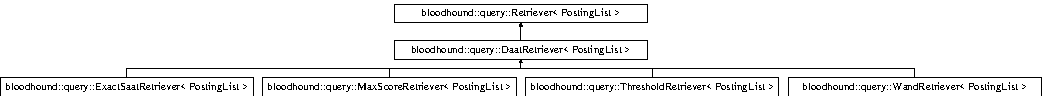
\includegraphics[height=1.296296cm]{classbloodhound_1_1query_1_1DaatRetriever}
\end{center}
\end{figure}
\subsection*{Classes}
\begin{DoxyCompactItemize}
\item 
struct \mbox{\hyperlink{structbloodhound_1_1query_1_1DaatRetriever_1_1IteratorPair}{Iterator\+Pair}}
\begin{DoxyCompactList}\small\item\em Current and end iterators of the same posting list. \end{DoxyCompactList}\end{DoxyCompactItemize}
\subsection*{Public Member Functions}
\begin{DoxyCompactItemize}
\item 
virtual \mbox{\hyperlink{classirk_1_1Heap}{irk\+::\+Heap}}$<$ \mbox{\hyperlink{structbloodhound_1_1Doc}{Doc}}, unsigned int $>$ \mbox{\hyperlink{classbloodhound_1_1query_1_1DaatRetriever_a6c292b0ca9feb30dbdb3a2799a34b3e5}{post\+\_\+lists\+\_\+by\+\_\+doc}} (const std\+::vector$<$ \mbox{\hyperlink{classbloodhound_1_1PostingList}{Posting\+List}} $>$ \&term\+\_\+postings)
\begin{DoxyCompactList}\small\item\em Returns initial min-\/heap of posting lists sorted by their current \mbox{\hyperlink{structbloodhound_1_1Doc}{Doc}}. \end{DoxyCompactList}\item 
virtual std\+::vector$<$ \mbox{\hyperlink{structbloodhound_1_1query_1_1DaatRetriever_1_1IteratorPair}{Iterator\+Pair}} $>$ \mbox{\hyperlink{classbloodhound_1_1query_1_1DaatRetriever_a5b10288f90a4fc4d89f56971bdc48363}{to\+\_\+iterators}} (const std\+::vector$<$ \mbox{\hyperlink{classbloodhound_1_1PostingList}{Posting\+List}} $>$ \&term\+\_\+postings)
\item 
virtual std\+::vector$<$ \mbox{\hyperlink{structbloodhound_1_1query_1_1Result}{Result}} $>$ \mbox{\hyperlink{classbloodhound_1_1query_1_1DaatRetriever_ab80b4867fc263827dc2fdbe0965a2e8c}{retrieve}} (const std\+::vector$<$ \mbox{\hyperlink{classbloodhound_1_1PostingList}{Posting\+List}} $>$ \&term\+\_\+postings, const std\+::vector$<$ \mbox{\hyperlink{structbloodhound_1_1Score}{Score}} $>$ \&term\+\_\+weights, std\+::size\+\_\+t k)
\begin{DoxyCompactList}\small\item\em Retrieves top-\/k results for the given posting lists and term weights. \end{DoxyCompactList}\end{DoxyCompactItemize}


\subsection{Detailed Description}
\subsubsection*{template$<$typename Posting\+List$>$\newline
class bloodhound\+::query\+::\+Daat\+Retriever$<$ Posting\+List $>$}

Document-\/at-\/a-\/time query processor. 

\subsection{Member Function Documentation}
\mbox{\Hypertarget{classbloodhound_1_1query_1_1DaatRetriever_a6c292b0ca9feb30dbdb3a2799a34b3e5}\label{classbloodhound_1_1query_1_1DaatRetriever_a6c292b0ca9feb30dbdb3a2799a34b3e5}} 
\index{bloodhound\+::query\+::\+Daat\+Retriever@{bloodhound\+::query\+::\+Daat\+Retriever}!post\+\_\+lists\+\_\+by\+\_\+doc@{post\+\_\+lists\+\_\+by\+\_\+doc}}
\index{post\+\_\+lists\+\_\+by\+\_\+doc@{post\+\_\+lists\+\_\+by\+\_\+doc}!bloodhound\+::query\+::\+Daat\+Retriever@{bloodhound\+::query\+::\+Daat\+Retriever}}
\subsubsection{\texorpdfstring{post\+\_\+lists\+\_\+by\+\_\+doc()}{post\_lists\_by\_doc()}}
{\footnotesize\ttfamily template$<$typename Posting\+List $>$ \\
virtual \mbox{\hyperlink{classirk_1_1Heap}{irk\+::\+Heap}}$<$\mbox{\hyperlink{structbloodhound_1_1Doc}{Doc}}, unsigned int$>$ \mbox{\hyperlink{classbloodhound_1_1query_1_1DaatRetriever}{bloodhound\+::query\+::\+Daat\+Retriever}}$<$ \mbox{\hyperlink{classbloodhound_1_1PostingList}{Posting\+List}} $>$\+::post\+\_\+lists\+\_\+by\+\_\+doc (\begin{DoxyParamCaption}\item[{const std\+::vector$<$ \mbox{\hyperlink{classbloodhound_1_1PostingList}{Posting\+List}} $>$ \&}]{term\+\_\+postings }\end{DoxyParamCaption})\hspace{0.3cm}{\ttfamily [inline]}, {\ttfamily [virtual]}}



Returns initial min-\/heap of posting lists sorted by their current \mbox{\hyperlink{structbloodhound_1_1Doc}{Doc}}. 

\mbox{\Hypertarget{classbloodhound_1_1query_1_1DaatRetriever_ab80b4867fc263827dc2fdbe0965a2e8c}\label{classbloodhound_1_1query_1_1DaatRetriever_ab80b4867fc263827dc2fdbe0965a2e8c}} 
\index{bloodhound\+::query\+::\+Daat\+Retriever@{bloodhound\+::query\+::\+Daat\+Retriever}!retrieve@{retrieve}}
\index{retrieve@{retrieve}!bloodhound\+::query\+::\+Daat\+Retriever@{bloodhound\+::query\+::\+Daat\+Retriever}}
\subsubsection{\texorpdfstring{retrieve()}{retrieve()}}
{\footnotesize\ttfamily template$<$typename Posting\+List $>$ \\
virtual std\+::vector$<$\mbox{\hyperlink{structbloodhound_1_1query_1_1Result}{Result}}$>$ \mbox{\hyperlink{classbloodhound_1_1query_1_1DaatRetriever}{bloodhound\+::query\+::\+Daat\+Retriever}}$<$ \mbox{\hyperlink{classbloodhound_1_1PostingList}{Posting\+List}} $>$\+::retrieve (\begin{DoxyParamCaption}\item[{const std\+::vector$<$ \mbox{\hyperlink{classbloodhound_1_1PostingList}{Posting\+List}} $>$ \&}]{term\+\_\+postings,  }\item[{const std\+::vector$<$ \mbox{\hyperlink{structbloodhound_1_1Score}{Score}} $>$ \&}]{term\+\_\+weights,  }\item[{std\+::size\+\_\+t}]{k }\end{DoxyParamCaption})\hspace{0.3cm}{\ttfamily [inline]}, {\ttfamily [virtual]}}



Retrieves top-\/k results for the given posting lists and term weights. 



Implements \mbox{\hyperlink{classbloodhound_1_1query_1_1Retriever_ae3c6a4628c5580e620c213b3dcd47c2b}{bloodhound\+::query\+::\+Retriever$<$ Posting\+List $>$}}.



Reimplemented in \mbox{\hyperlink{classbloodhound_1_1query_1_1WandRetriever_a5f3068bc363c16c5b7255a925ea5af8c}{bloodhound\+::query\+::\+Wand\+Retriever$<$ Posting\+List $>$}}, \mbox{\hyperlink{classbloodhound_1_1query_1_1ThresholdRetriever_a06750450e1246e755ebad2d5dac6e8a8}{bloodhound\+::query\+::\+Threshold\+Retriever$<$ Posting\+List $>$}}, and \mbox{\hyperlink{classbloodhound_1_1query_1_1ExactSaatRetriever_aced2763cc2a4c12838fef4a20759049e}{bloodhound\+::query\+::\+Exact\+Saat\+Retriever$<$ Posting\+List $>$}}.

\mbox{\Hypertarget{classbloodhound_1_1query_1_1DaatRetriever_a5b10288f90a4fc4d89f56971bdc48363}\label{classbloodhound_1_1query_1_1DaatRetriever_a5b10288f90a4fc4d89f56971bdc48363}} 
\index{bloodhound\+::query\+::\+Daat\+Retriever@{bloodhound\+::query\+::\+Daat\+Retriever}!to\+\_\+iterators@{to\+\_\+iterators}}
\index{to\+\_\+iterators@{to\+\_\+iterators}!bloodhound\+::query\+::\+Daat\+Retriever@{bloodhound\+::query\+::\+Daat\+Retriever}}
\subsubsection{\texorpdfstring{to\+\_\+iterators()}{to\_iterators()}}
{\footnotesize\ttfamily template$<$typename Posting\+List $>$ \\
virtual std\+::vector$<$\mbox{\hyperlink{structbloodhound_1_1query_1_1DaatRetriever_1_1IteratorPair}{Iterator\+Pair}}$>$ \mbox{\hyperlink{classbloodhound_1_1query_1_1DaatRetriever}{bloodhound\+::query\+::\+Daat\+Retriever}}$<$ \mbox{\hyperlink{classbloodhound_1_1PostingList}{Posting\+List}} $>$\+::to\+\_\+iterators (\begin{DoxyParamCaption}\item[{const std\+::vector$<$ \mbox{\hyperlink{classbloodhound_1_1PostingList}{Posting\+List}} $>$ \&}]{term\+\_\+postings }\end{DoxyParamCaption})\hspace{0.3cm}{\ttfamily [inline]}, {\ttfamily [virtual]}}



The documentation for this class was generated from the following file\+:\begin{DoxyCompactItemize}
\item 
include/\mbox{\hyperlink{retrievers_8hpp}{retrievers.\+hpp}}\end{DoxyCompactItemize}

\hypertarget{structbloodhound_1_1query_1_1debug}{}\section{bloodhound\+:\+:query\+:\+:debug Struct Reference}
\label{structbloodhound_1_1query_1_1debug}\index{bloodhound\+::query\+::debug@{bloodhound\+::query\+::debug}}


{\ttfamily \#include $<$query.\+hpp$>$}

Inheritance diagram for bloodhound\+:\+:query\+:\+:debug\+:\begin{figure}[H]
\begin{center}
\leavevmode
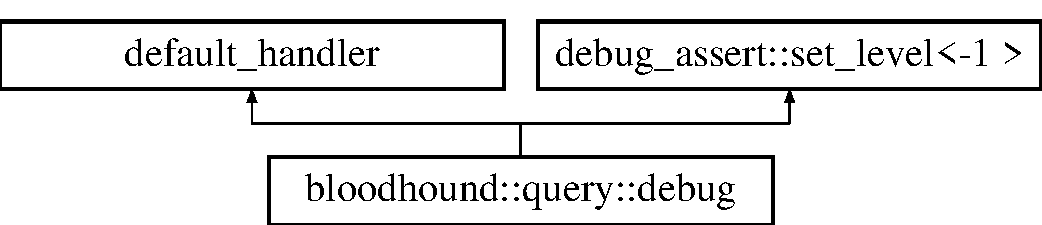
\includegraphics[height=2.000000cm]{structbloodhound_1_1query_1_1debug}
\end{center}
\end{figure}


The documentation for this struct was generated from the following file\+:\begin{DoxyCompactItemize}
\item 
include/\mbox{\hyperlink{query_8hpp}{query.\+hpp}}\end{DoxyCompactItemize}

\hypertarget{structbloodhound_1_1Doc}{}\section{bloodhound\+:\+:Doc Struct Reference}
\label{structbloodhound_1_1Doc}\index{bloodhound\+::\+Doc@{bloodhound\+::\+Doc}}


{\ttfamily \#include $<$index.\+hpp$>$}

Inheritance diagram for bloodhound\+:\+:Doc\+:\begin{figure}[H]
\begin{center}
\leavevmode
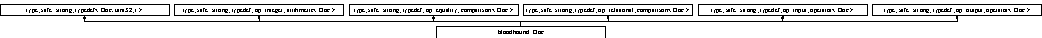
\includegraphics[height=0.514233cm]{structbloodhound_1_1Doc}
\end{center}
\end{figure}
\subsection*{Public Member Functions}
\begin{DoxyCompactItemize}
\item 
\mbox{\hyperlink{structbloodhound_1_1Doc_afb469079253eb5b66e0b613f873ae81d}{operator std\+::size\+\_\+t}} () const
\end{DoxyCompactItemize}


\subsection{Member Function Documentation}
\mbox{\Hypertarget{structbloodhound_1_1Doc_afb469079253eb5b66e0b613f873ae81d}\label{structbloodhound_1_1Doc_afb469079253eb5b66e0b613f873ae81d}} 
\index{bloodhound\+::\+Doc@{bloodhound\+::\+Doc}!operator std\+::size\+\_\+t@{operator std\+::size\+\_\+t}}
\index{operator std\+::size\+\_\+t@{operator std\+::size\+\_\+t}!bloodhound\+::\+Doc@{bloodhound\+::\+Doc}}
\subsubsection{\texorpdfstring{operator std\+::size\+\_\+t()}{operator std::size\_t()}}
{\footnotesize\ttfamily bloodhound\+::\+Doc\+::operator std\+::size\+\_\+t (\begin{DoxyParamCaption}{ }\end{DoxyParamCaption}) const\hspace{0.3cm}{\ttfamily [inline]}}



The documentation for this struct was generated from the following file\+:\begin{DoxyCompactItemize}
\item 
include/\mbox{\hyperlink{index_8hpp}{index.\+hpp}}\end{DoxyCompactItemize}

\hypertarget{structbloodhound_1_1doc__equal__to}{}\section{bloodhound\+:\+:doc\+\_\+equal\+\_\+to$<$ Posting $>$ Struct Template Reference}
\label{structbloodhound_1_1doc__equal__to}\index{bloodhound\+::doc\+\_\+equal\+\_\+to$<$ Posting $>$@{bloodhound\+::doc\+\_\+equal\+\_\+to$<$ Posting $>$}}


{\ttfamily \#include $<$index.\+hpp$>$}

\subsection*{Public Member Functions}
\begin{DoxyCompactItemize}
\item 
bool \mbox{\hyperlink{structbloodhound_1_1doc__equal__to_a5a8e28107bb693527fa4c513b3678b1b}{operator()}} (const \mbox{\hyperlink{structbloodhound_1_1Posting}{Posting}} \&lhs, const \mbox{\hyperlink{structbloodhound_1_1Posting}{Posting}} \&rhs)
\end{DoxyCompactItemize}


\subsection{Member Function Documentation}
\mbox{\Hypertarget{structbloodhound_1_1doc__equal__to_a5a8e28107bb693527fa4c513b3678b1b}\label{structbloodhound_1_1doc__equal__to_a5a8e28107bb693527fa4c513b3678b1b}} 
\index{bloodhound\+::doc\+\_\+equal\+\_\+to@{bloodhound\+::doc\+\_\+equal\+\_\+to}!operator()@{operator()}}
\index{operator()@{operator()}!bloodhound\+::doc\+\_\+equal\+\_\+to@{bloodhound\+::doc\+\_\+equal\+\_\+to}}
\subsubsection{\texorpdfstring{operator()()}{operator()()}}
{\footnotesize\ttfamily template$<$class Posting $>$ \\
bool \mbox{\hyperlink{structbloodhound_1_1doc__equal__to}{bloodhound\+::doc\+\_\+equal\+\_\+to}}$<$ \mbox{\hyperlink{structbloodhound_1_1Posting}{Posting}} $>$\+::operator() (\begin{DoxyParamCaption}\item[{const \mbox{\hyperlink{structbloodhound_1_1Posting}{Posting}} \&}]{lhs,  }\item[{const \mbox{\hyperlink{structbloodhound_1_1Posting}{Posting}} \&}]{rhs }\end{DoxyParamCaption})\hspace{0.3cm}{\ttfamily [inline]}}



The documentation for this struct was generated from the following file\+:\begin{DoxyCompactItemize}
\item 
include/\mbox{\hyperlink{index_8hpp}{index.\+hpp}}\end{DoxyCompactItemize}

\hypertarget{classbloodhound_1_1query_1_1ExactSaatRetriever}{}\section{bloodhound\+:\+:query\+:\+:Exact\+Saat\+Retriever$<$ Posting\+List $>$ Class Template Reference}
\label{classbloodhound_1_1query_1_1ExactSaatRetriever}\index{bloodhound\+::query\+::\+Exact\+Saat\+Retriever$<$ Posting\+List $>$@{bloodhound\+::query\+::\+Exact\+Saat\+Retriever$<$ Posting\+List $>$}}


{\ttfamily \#include $<$saat.\+hpp$>$}

Inheritance diagram for bloodhound\+:\+:query\+:\+:Exact\+Saat\+Retriever$<$ Posting\+List $>$\+:\begin{figure}[H]
\begin{center}
\leavevmode
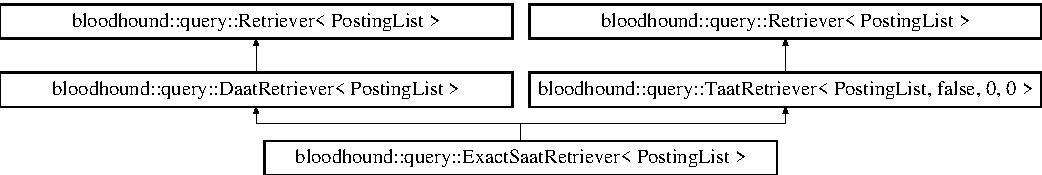
\includegraphics[height=2.346369cm]{classbloodhound_1_1query_1_1ExactSaatRetriever}
\end{center}
\end{figure}
\subsection*{Public Member Functions}
\begin{DoxyCompactItemize}
\item 
\hyperlink{classbloodhound_1_1query_1_1ExactSaatRetriever_a50c5c53b4b7aff76e4eabf040219be52}{Exact\+Saat\+Retriever} (std\+::size\+\_\+t collection\+\_\+size, double et\+\_\+threshold=1.\+0)
\item 
std\+::size\+\_\+t \hyperlink{classbloodhound_1_1query_1_1ExactSaatRetriever_a21f4192190392fee8d8b12b99c6bbe0e}{count\+\_\+postings} (const std\+::vector$<$ \hyperlink{classbloodhound_1_1PostingList}{Posting\+List} $>$ \&term\+\_\+postings)
\item 
virtual irkit\+::\+Heap$<$ \hyperlink{structbloodhound_1_1Score}{Score}, unsigned int $>$ \hyperlink{classbloodhound_1_1query_1_1ExactSaatRetriever_a180277ad96862e92c102066586edc74f}{post\+\_\+lists\+\_\+by\+\_\+score} (const std\+::vector$<$ \hyperlink{classbloodhound_1_1PostingList}{Posting\+List} $>$ \&term\+\_\+postings, const std\+::vector$<$ \hyperlink{structbloodhound_1_1Score}{Score} $>$ \&term\+\_\+weights)
\item 
virtual std\+::vector$<$ \hyperlink{structbloodhound_1_1query_1_1Result}{Result} $>$ \hyperlink{classbloodhound_1_1query_1_1ExactSaatRetriever_aced2763cc2a4c12838fef4a20759049e}{retrieve} (const std\+::vector$<$ \hyperlink{classbloodhound_1_1PostingList}{Posting\+List} $>$ \&term\+\_\+postings, const std\+::vector$<$ \hyperlink{structbloodhound_1_1Score}{Score} $>$ \&term\+\_\+weights, std\+::size\+\_\+t k)
\begin{DoxyCompactList}\small\item\em Retrieves top-\/k results for the given posting lists and term weights. \end{DoxyCompactList}\item 
std\+::size\+\_\+t \hyperlink{classbloodhound_1_1query_1_1ExactSaatRetriever_a1cf3c5e50a72880e1eb8d995ff22b20a}{get\+\_\+processed\+\_\+postings} ()
\item 
std\+::size\+\_\+t \hyperlink{classbloodhound_1_1query_1_1ExactSaatRetriever_a5d3a882f8f117130a4be46e711397e3c}{get\+\_\+posting\+\_\+threshold} ()
\item 
std\+::size\+\_\+t \hyperlink{classbloodhound_1_1query_1_1ExactSaatRetriever_a43b6bd8cdc3a64c5eabf778230c53419}{get\+\_\+posting\+\_\+count} ()
\item 
void \hyperlink{classbloodhound_1_1query_1_1ExactSaatRetriever_a78016cfffe921ed440dec62c6f82f4cc}{set\+\_\+et\+\_\+threshold} (double et)
\item 
virtual nlohmann\+::json \hyperlink{classbloodhound_1_1query_1_1ExactSaatRetriever_a716838f463f124964e76f48bc37d32cc}{stats} ()
\end{DoxyCompactItemize}
\subsection*{Additional Inherited Members}


\subsection{Constructor \& Destructor Documentation}
\mbox{\Hypertarget{classbloodhound_1_1query_1_1ExactSaatRetriever_a50c5c53b4b7aff76e4eabf040219be52}\label{classbloodhound_1_1query_1_1ExactSaatRetriever_a50c5c53b4b7aff76e4eabf040219be52}} 
\index{bloodhound\+::query\+::\+Exact\+Saat\+Retriever@{bloodhound\+::query\+::\+Exact\+Saat\+Retriever}!Exact\+Saat\+Retriever@{Exact\+Saat\+Retriever}}
\index{Exact\+Saat\+Retriever@{Exact\+Saat\+Retriever}!bloodhound\+::query\+::\+Exact\+Saat\+Retriever@{bloodhound\+::query\+::\+Exact\+Saat\+Retriever}}
\subsubsection{\texorpdfstring{Exact\+Saat\+Retriever()}{ExactSaatRetriever()}}
{\footnotesize\ttfamily template$<$typename Posting\+List $>$ \\
\hyperlink{classbloodhound_1_1query_1_1ExactSaatRetriever}{bloodhound\+::query\+::\+Exact\+Saat\+Retriever}$<$ \hyperlink{classbloodhound_1_1PostingList}{Posting\+List} $>$\+::\hyperlink{classbloodhound_1_1query_1_1ExactSaatRetriever}{Exact\+Saat\+Retriever} (\begin{DoxyParamCaption}\item[{std\+::size\+\_\+t}]{collection\+\_\+size,  }\item[{double}]{et\+\_\+threshold = {\ttfamily 1.0} }\end{DoxyParamCaption})\hspace{0.3cm}{\ttfamily [inline]}}



\subsection{Member Function Documentation}
\mbox{\Hypertarget{classbloodhound_1_1query_1_1ExactSaatRetriever_a21f4192190392fee8d8b12b99c6bbe0e}\label{classbloodhound_1_1query_1_1ExactSaatRetriever_a21f4192190392fee8d8b12b99c6bbe0e}} 
\index{bloodhound\+::query\+::\+Exact\+Saat\+Retriever@{bloodhound\+::query\+::\+Exact\+Saat\+Retriever}!count\+\_\+postings@{count\+\_\+postings}}
\index{count\+\_\+postings@{count\+\_\+postings}!bloodhound\+::query\+::\+Exact\+Saat\+Retriever@{bloodhound\+::query\+::\+Exact\+Saat\+Retriever}}
\subsubsection{\texorpdfstring{count\+\_\+postings()}{count\_postings()}}
{\footnotesize\ttfamily template$<$typename Posting\+List $>$ \\
std\+::size\+\_\+t \hyperlink{classbloodhound_1_1query_1_1ExactSaatRetriever}{bloodhound\+::query\+::\+Exact\+Saat\+Retriever}$<$ \hyperlink{classbloodhound_1_1PostingList}{Posting\+List} $>$\+::count\+\_\+postings (\begin{DoxyParamCaption}\item[{const std\+::vector$<$ \hyperlink{classbloodhound_1_1PostingList}{Posting\+List} $>$ \&}]{term\+\_\+postings }\end{DoxyParamCaption})\hspace{0.3cm}{\ttfamily [inline]}}

\mbox{\Hypertarget{classbloodhound_1_1query_1_1ExactSaatRetriever_a43b6bd8cdc3a64c5eabf778230c53419}\label{classbloodhound_1_1query_1_1ExactSaatRetriever_a43b6bd8cdc3a64c5eabf778230c53419}} 
\index{bloodhound\+::query\+::\+Exact\+Saat\+Retriever@{bloodhound\+::query\+::\+Exact\+Saat\+Retriever}!get\+\_\+posting\+\_\+count@{get\+\_\+posting\+\_\+count}}
\index{get\+\_\+posting\+\_\+count@{get\+\_\+posting\+\_\+count}!bloodhound\+::query\+::\+Exact\+Saat\+Retriever@{bloodhound\+::query\+::\+Exact\+Saat\+Retriever}}
\subsubsection{\texorpdfstring{get\+\_\+posting\+\_\+count()}{get\_posting\_count()}}
{\footnotesize\ttfamily template$<$typename Posting\+List $>$ \\
std\+::size\+\_\+t \hyperlink{classbloodhound_1_1query_1_1ExactSaatRetriever}{bloodhound\+::query\+::\+Exact\+Saat\+Retriever}$<$ \hyperlink{classbloodhound_1_1PostingList}{Posting\+List} $>$\+::get\+\_\+posting\+\_\+count (\begin{DoxyParamCaption}{ }\end{DoxyParamCaption})\hspace{0.3cm}{\ttfamily [inline]}}

\mbox{\Hypertarget{classbloodhound_1_1query_1_1ExactSaatRetriever_a5d3a882f8f117130a4be46e711397e3c}\label{classbloodhound_1_1query_1_1ExactSaatRetriever_a5d3a882f8f117130a4be46e711397e3c}} 
\index{bloodhound\+::query\+::\+Exact\+Saat\+Retriever@{bloodhound\+::query\+::\+Exact\+Saat\+Retriever}!get\+\_\+posting\+\_\+threshold@{get\+\_\+posting\+\_\+threshold}}
\index{get\+\_\+posting\+\_\+threshold@{get\+\_\+posting\+\_\+threshold}!bloodhound\+::query\+::\+Exact\+Saat\+Retriever@{bloodhound\+::query\+::\+Exact\+Saat\+Retriever}}
\subsubsection{\texorpdfstring{get\+\_\+posting\+\_\+threshold()}{get\_posting\_threshold()}}
{\footnotesize\ttfamily template$<$typename Posting\+List $>$ \\
std\+::size\+\_\+t \hyperlink{classbloodhound_1_1query_1_1ExactSaatRetriever}{bloodhound\+::query\+::\+Exact\+Saat\+Retriever}$<$ \hyperlink{classbloodhound_1_1PostingList}{Posting\+List} $>$\+::get\+\_\+posting\+\_\+threshold (\begin{DoxyParamCaption}{ }\end{DoxyParamCaption})\hspace{0.3cm}{\ttfamily [inline]}}

\mbox{\Hypertarget{classbloodhound_1_1query_1_1ExactSaatRetriever_a1cf3c5e50a72880e1eb8d995ff22b20a}\label{classbloodhound_1_1query_1_1ExactSaatRetriever_a1cf3c5e50a72880e1eb8d995ff22b20a}} 
\index{bloodhound\+::query\+::\+Exact\+Saat\+Retriever@{bloodhound\+::query\+::\+Exact\+Saat\+Retriever}!get\+\_\+processed\+\_\+postings@{get\+\_\+processed\+\_\+postings}}
\index{get\+\_\+processed\+\_\+postings@{get\+\_\+processed\+\_\+postings}!bloodhound\+::query\+::\+Exact\+Saat\+Retriever@{bloodhound\+::query\+::\+Exact\+Saat\+Retriever}}
\subsubsection{\texorpdfstring{get\+\_\+processed\+\_\+postings()}{get\_processed\_postings()}}
{\footnotesize\ttfamily template$<$typename Posting\+List $>$ \\
std\+::size\+\_\+t \hyperlink{classbloodhound_1_1query_1_1ExactSaatRetriever}{bloodhound\+::query\+::\+Exact\+Saat\+Retriever}$<$ \hyperlink{classbloodhound_1_1PostingList}{Posting\+List} $>$\+::get\+\_\+processed\+\_\+postings (\begin{DoxyParamCaption}{ }\end{DoxyParamCaption})\hspace{0.3cm}{\ttfamily [inline]}}

\mbox{\Hypertarget{classbloodhound_1_1query_1_1ExactSaatRetriever_a180277ad96862e92c102066586edc74f}\label{classbloodhound_1_1query_1_1ExactSaatRetriever_a180277ad96862e92c102066586edc74f}} 
\index{bloodhound\+::query\+::\+Exact\+Saat\+Retriever@{bloodhound\+::query\+::\+Exact\+Saat\+Retriever}!post\+\_\+lists\+\_\+by\+\_\+score@{post\+\_\+lists\+\_\+by\+\_\+score}}
\index{post\+\_\+lists\+\_\+by\+\_\+score@{post\+\_\+lists\+\_\+by\+\_\+score}!bloodhound\+::query\+::\+Exact\+Saat\+Retriever@{bloodhound\+::query\+::\+Exact\+Saat\+Retriever}}
\subsubsection{\texorpdfstring{post\+\_\+lists\+\_\+by\+\_\+score()}{post\_lists\_by\_score()}}
{\footnotesize\ttfamily template$<$typename Posting\+List $>$ \\
virtual irkit\+::\+Heap$<$\hyperlink{structbloodhound_1_1Score}{Score}, unsigned int$>$ \hyperlink{classbloodhound_1_1query_1_1ExactSaatRetriever}{bloodhound\+::query\+::\+Exact\+Saat\+Retriever}$<$ \hyperlink{classbloodhound_1_1PostingList}{Posting\+List} $>$\+::post\+\_\+lists\+\_\+by\+\_\+score (\begin{DoxyParamCaption}\item[{const std\+::vector$<$ \hyperlink{classbloodhound_1_1PostingList}{Posting\+List} $>$ \&}]{term\+\_\+postings,  }\item[{const std\+::vector$<$ \hyperlink{structbloodhound_1_1Score}{Score} $>$ \&}]{term\+\_\+weights }\end{DoxyParamCaption})\hspace{0.3cm}{\ttfamily [inline]}, {\ttfamily [virtual]}}

\mbox{\Hypertarget{classbloodhound_1_1query_1_1ExactSaatRetriever_aced2763cc2a4c12838fef4a20759049e}\label{classbloodhound_1_1query_1_1ExactSaatRetriever_aced2763cc2a4c12838fef4a20759049e}} 
\index{bloodhound\+::query\+::\+Exact\+Saat\+Retriever@{bloodhound\+::query\+::\+Exact\+Saat\+Retriever}!retrieve@{retrieve}}
\index{retrieve@{retrieve}!bloodhound\+::query\+::\+Exact\+Saat\+Retriever@{bloodhound\+::query\+::\+Exact\+Saat\+Retriever}}
\subsubsection{\texorpdfstring{retrieve()}{retrieve()}}
{\footnotesize\ttfamily template$<$typename Posting\+List $>$ \\
virtual std\+::vector$<$\hyperlink{structbloodhound_1_1query_1_1Result}{Result}$>$ \hyperlink{classbloodhound_1_1query_1_1ExactSaatRetriever}{bloodhound\+::query\+::\+Exact\+Saat\+Retriever}$<$ \hyperlink{classbloodhound_1_1PostingList}{Posting\+List} $>$\+::retrieve (\begin{DoxyParamCaption}\item[{const std\+::vector$<$ \hyperlink{classbloodhound_1_1PostingList}{Posting\+List} $>$ \&}]{term\+\_\+postings,  }\item[{const std\+::vector$<$ \hyperlink{structbloodhound_1_1Score}{Score} $>$ \&}]{term\+\_\+weights,  }\item[{std\+::size\+\_\+t}]{k }\end{DoxyParamCaption})\hspace{0.3cm}{\ttfamily [inline]}, {\ttfamily [virtual]}}



Retrieves top-\/k results for the given posting lists and term weights. 



Reimplemented from \hyperlink{classbloodhound_1_1query_1_1DaatRetriever_ab80b4867fc263827dc2fdbe0965a2e8c}{bloodhound\+::query\+::\+Daat\+Retriever$<$ Posting\+List $>$}.

\mbox{\Hypertarget{classbloodhound_1_1query_1_1ExactSaatRetriever_a78016cfffe921ed440dec62c6f82f4cc}\label{classbloodhound_1_1query_1_1ExactSaatRetriever_a78016cfffe921ed440dec62c6f82f4cc}} 
\index{bloodhound\+::query\+::\+Exact\+Saat\+Retriever@{bloodhound\+::query\+::\+Exact\+Saat\+Retriever}!set\+\_\+et\+\_\+threshold@{set\+\_\+et\+\_\+threshold}}
\index{set\+\_\+et\+\_\+threshold@{set\+\_\+et\+\_\+threshold}!bloodhound\+::query\+::\+Exact\+Saat\+Retriever@{bloodhound\+::query\+::\+Exact\+Saat\+Retriever}}
\subsubsection{\texorpdfstring{set\+\_\+et\+\_\+threshold()}{set\_et\_threshold()}}
{\footnotesize\ttfamily template$<$typename Posting\+List $>$ \\
void \hyperlink{classbloodhound_1_1query_1_1ExactSaatRetriever}{bloodhound\+::query\+::\+Exact\+Saat\+Retriever}$<$ \hyperlink{classbloodhound_1_1PostingList}{Posting\+List} $>$\+::set\+\_\+et\+\_\+threshold (\begin{DoxyParamCaption}\item[{double}]{et }\end{DoxyParamCaption})\hspace{0.3cm}{\ttfamily [inline]}}

\mbox{\Hypertarget{classbloodhound_1_1query_1_1ExactSaatRetriever_a716838f463f124964e76f48bc37d32cc}\label{classbloodhound_1_1query_1_1ExactSaatRetriever_a716838f463f124964e76f48bc37d32cc}} 
\index{bloodhound\+::query\+::\+Exact\+Saat\+Retriever@{bloodhound\+::query\+::\+Exact\+Saat\+Retriever}!stats@{stats}}
\index{stats@{stats}!bloodhound\+::query\+::\+Exact\+Saat\+Retriever@{bloodhound\+::query\+::\+Exact\+Saat\+Retriever}}
\subsubsection{\texorpdfstring{stats()}{stats()}}
{\footnotesize\ttfamily template$<$typename Posting\+List $>$ \\
virtual nlohmann\+::json \hyperlink{classbloodhound_1_1query_1_1ExactSaatRetriever}{bloodhound\+::query\+::\+Exact\+Saat\+Retriever}$<$ \hyperlink{classbloodhound_1_1PostingList}{Posting\+List} $>$\+::stats (\begin{DoxyParamCaption}{ }\end{DoxyParamCaption})\hspace{0.3cm}{\ttfamily [inline]}, {\ttfamily [virtual]}}



Reimplemented from \hyperlink{classbloodhound_1_1query_1_1Retriever_a58da32a5139b980ba874f8b5e6bb89ec}{bloodhound\+::query\+::\+Retriever$<$ Posting\+List $>$}.



The documentation for this class was generated from the following file\+:\begin{DoxyCompactItemize}
\item 
include/\hyperlink{saat_8hpp}{saat.\+hpp}\end{DoxyCompactItemize}

\hypertarget{structbloodhound_1_1query_1_1has__iterator}{}\section{bloodhound\+:\+:query\+:\+:has\+\_\+iterator$<$ T, typename $>$ Struct Template Reference}
\label{structbloodhound_1_1query_1_1has__iterator}\index{bloodhound\+::query\+::has\+\_\+iterator$<$ T, typename $>$@{bloodhound\+::query\+::has\+\_\+iterator$<$ T, typename $>$}}


{\ttfamily \#include $<$query.\+hpp$>$}

Inheritance diagram for bloodhound\+:\+:query\+:\+:has\+\_\+iterator$<$ T, typename $>$\+:\begin{figure}[H]
\begin{center}
\leavevmode
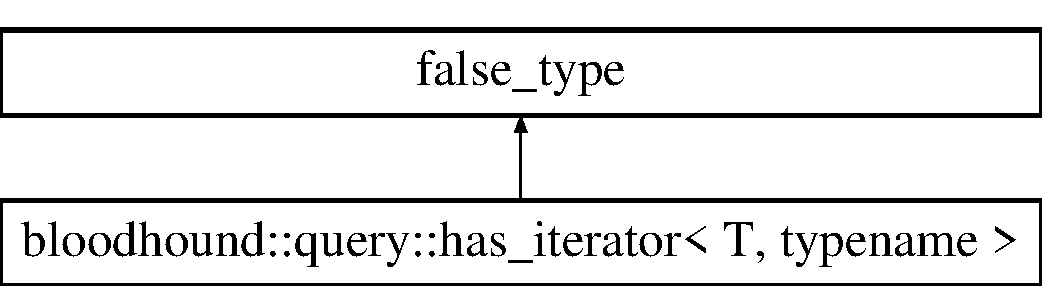
\includegraphics[height=2.000000cm]{structbloodhound_1_1query_1_1has__iterator}
\end{center}
\end{figure}


The documentation for this struct was generated from the following file\+:\begin{DoxyCompactItemize}
\item 
include/\mbox{\hyperlink{query_8hpp}{query.\+hpp}}\end{DoxyCompactItemize}

\hypertarget{structbloodhound_1_1query_1_1has__iterator_3_01T_00_01void__t_3_01typename_01T_1_1iterator_01_4_01_4}{}\section{bloodhound\+:\+:query\+:\+:has\+\_\+iterator$<$ T, void\+\_\+t$<$ typename T\+:\+:iterator $>$ $>$ Struct Template Reference}
\label{structbloodhound_1_1query_1_1has__iterator_3_01T_00_01void__t_3_01typename_01T_1_1iterator_01_4_01_4}\index{bloodhound\+::query\+::has\+\_\+iterator$<$ T, void\+\_\+t$<$ typename T\+::iterator $>$ $>$@{bloodhound\+::query\+::has\+\_\+iterator$<$ T, void\+\_\+t$<$ typename T\+::iterator $>$ $>$}}


{\ttfamily \#include $<$query.\+hpp$>$}

Inheritance diagram for bloodhound\+:\+:query\+:\+:has\+\_\+iterator$<$ T, void\+\_\+t$<$ typename T\+:\+:iterator $>$ $>$\+:\begin{figure}[H]
\begin{center}
\leavevmode
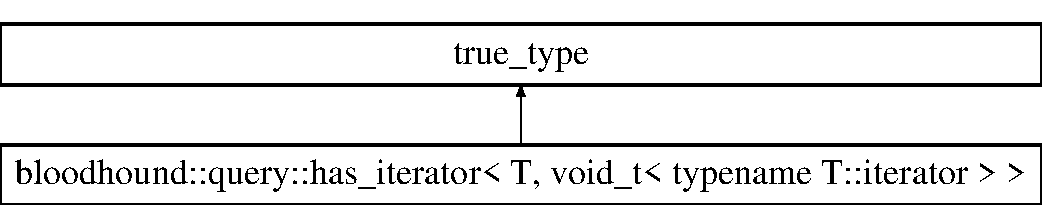
\includegraphics[height=2.000000cm]{structbloodhound_1_1query_1_1has__iterator_3_01T_00_01void__t_3_01typename_01T_1_1iterator_01_4_01_4}
\end{center}
\end{figure}


The documentation for this struct was generated from the following file\+:\begin{DoxyCompactItemize}
\item 
include/\mbox{\hyperlink{query_8hpp}{query.\+hpp}}\end{DoxyCompactItemize}

\hypertarget{structbloodhound_1_1query_1_1has__posting__iterator}{}\section{bloodhound\+:\+:query\+:\+:has\+\_\+posting\+\_\+iterator$<$ T, typename $>$ Struct Template Reference}
\label{structbloodhound_1_1query_1_1has__posting__iterator}\index{bloodhound\+::query\+::has\+\_\+posting\+\_\+iterator$<$ T, typename $>$@{bloodhound\+::query\+::has\+\_\+posting\+\_\+iterator$<$ T, typename $>$}}


{\ttfamily \#include $<$query.\+hpp$>$}

Inheritance diagram for bloodhound\+:\+:query\+:\+:has\+\_\+posting\+\_\+iterator$<$ T, typename $>$\+:\begin{figure}[H]
\begin{center}
\leavevmode
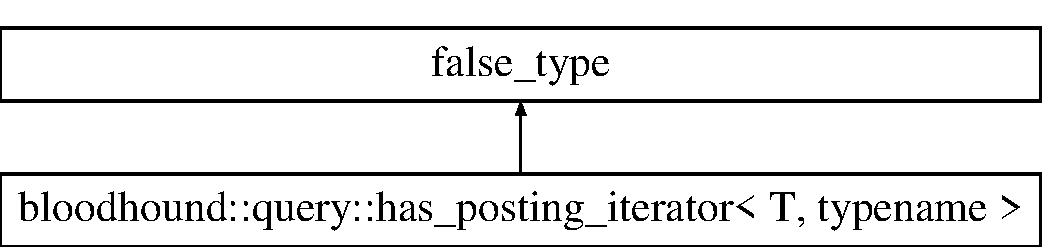
\includegraphics[height=2.000000cm]{structbloodhound_1_1query_1_1has__posting__iterator}
\end{center}
\end{figure}


The documentation for this struct was generated from the following file\+:\begin{DoxyCompactItemize}
\item 
include/\mbox{\hyperlink{query_8hpp}{query.\+hpp}}\end{DoxyCompactItemize}

\hypertarget{structbloodhound_1_1query_1_1has__posting__iterator_3_01T_00_01std_1_1enable__if__t_3_01std_1_1i3aad327a30d60305d06d5c73680c1a38}{}\section{bloodhound\+:\+:query\+:\+:has\+\_\+posting\+\_\+iterator$<$ T, std\+:\+:enable\+\_\+if\+\_\+t$<$ std\+:\+:is\+\_\+convertible$<$ decltype(std\+:\+:declval$<$ T \& $>$().end()), typename T\+:\+:iterator $>$\+:\+:value \&\&std\+:\+:is\+\_\+convertible$<$ decltype(std\+:\+:declval$<$ T \& $>$().begin()), typename T\+:\+:iterator $>$\+:\+:value \&\&std\+:\+:is\+\_\+convertible$<$ decltype($\ast$std\+:\+:declval$<$ T \& $>$().begin()), Posting \& $>$\+:\+:value \&\&std\+:\+:is\+\_\+convertible$<$ decltype($\ast$std\+:\+:declval$<$ T \& $>$().end()), Posting \& $>$\+:\+:value $>$ $>$ Struct Template Reference}
\label{structbloodhound_1_1query_1_1has__posting__iterator_3_01T_00_01std_1_1enable__if__t_3_01std_1_1i3aad327a30d60305d06d5c73680c1a38}\index{bloodhound\+::query\+::has\+\_\+posting\+\_\+iterator$<$ T, std\+::enable\+\_\+if\+\_\+t$<$ std\+::is\+\_\+convertible$<$ decltype(std\+::declval$<$ T \& $>$().\+end()), typename T\+::iterator $>$\+::value \&\&std\+::is\+\_\+convertible$<$ decltype(std\+::declval$<$ T \& $>$().\+begin()), typename T\+::iterator $>$\+::value \&\&std\+::is\+\_\+convertible$<$ decltype($\ast$std\+::declval$<$ T \& $>$().\+begin()), Posting \& $>$\+::value \&\&std\+::is\+\_\+convertible$<$ decltype($\ast$std\+::declval$<$ T \& $>$().\+end()), Posting \& $>$\+::value $>$ $>$@{bloodhound\+::query\+::has\+\_\+posting\+\_\+iterator$<$ T, std\+::enable\+\_\+if\+\_\+t$<$ std\+::is\+\_\+convertible$<$ decltype(std\+::declval$<$ T \& $>$().\+end()), typename T\+::iterator $>$\+::value \&\&std\+::is\+\_\+convertible$<$ decltype(std\+::declval$<$ T \& $>$().\+begin()), typename T\+::iterator $>$\+::value \&\&std\+::is\+\_\+convertible$<$ decltype($\ast$std\+::declval$<$ T \& $>$().\+begin()), Posting \& $>$\+::value \&\&std\+::is\+\_\+convertible$<$ decltype($\ast$std\+::declval$<$ T \& $>$().\+end()), Posting \& $>$\+::value $>$ $>$}}


{\ttfamily \#include $<$query.\+hpp$>$}

Inheritance diagram for bloodhound\+:\+:query\+:\+:has\+\_\+posting\+\_\+iterator$<$ T, std\+:\+:enable\+\_\+if\+\_\+t$<$ std\+:\+:is\+\_\+convertible$<$ decltype(std\+:\+:declval$<$ T \& $>$().end()), typename T\+:\+:iterator $>$\+:\+:value \&\&std\+:\+:is\+\_\+convertible$<$ decltype(std\+:\+:declval$<$ T \& $>$().begin()), typename T\+:\+:iterator $>$\+:\+:value \&\&std\+:\+:is\+\_\+convertible$<$ decltype($\ast$std\+:\+:declval$<$ T \& $>$().begin()), Posting \& $>$\+:\+:value \&\&std\+:\+:is\+\_\+convertible$<$ decltype($\ast$std\+:\+:declval$<$ T \& $>$().end()), Posting \& $>$\+:\+:value $>$ $>$\+:\begin{figure}[H]
\begin{center}
\leavevmode
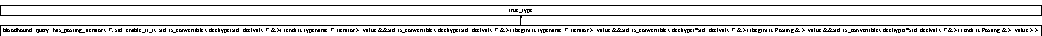
\includegraphics[height=0.480069cm]{structbloodhound_1_1query_1_1has__posting__iterator_3_01T_00_01std_1_1enable__if__t_3_01std_1_1i3aad327a30d60305d06d5c73680c1a38}
\end{center}
\end{figure}


The documentation for this struct was generated from the following file\+:\begin{DoxyCompactItemize}
\item 
include/\mbox{\hyperlink{query_8hpp}{query.\+hpp}}\end{DoxyCompactItemize}

\hypertarget{structstd_1_1hash_3_01bloodhound_1_1Doc_01_4}{}\section{std\+:\+:hash$<$ bloodhound\+:\+:Doc $>$ Struct Template Reference}
\label{structstd_1_1hash_3_01bloodhound_1_1Doc_01_4}\index{std\+::hash$<$ bloodhound\+::\+Doc $>$@{std\+::hash$<$ bloodhound\+::\+Doc $>$}}


{\ttfamily \#include $<$index.\+hpp$>$}

\subsection*{Public Member Functions}
\begin{DoxyCompactItemize}
\item 
std\+::size\+\_\+t \mbox{\hyperlink{structstd_1_1hash_3_01bloodhound_1_1Doc_01_4_a3f89deb7b2548010c7f3b63afc9d7fa4}{operator()}} (\mbox{\hyperlink{structbloodhound_1_1Doc}{bloodhound\+::\+Doc}} const \&t) const noexcept
\end{DoxyCompactItemize}


\subsection{Member Function Documentation}
\mbox{\Hypertarget{structstd_1_1hash_3_01bloodhound_1_1Doc_01_4_a3f89deb7b2548010c7f3b63afc9d7fa4}\label{structstd_1_1hash_3_01bloodhound_1_1Doc_01_4_a3f89deb7b2548010c7f3b63afc9d7fa4}} 
\index{std\+::hash$<$ bloodhound\+::\+Doc $>$@{std\+::hash$<$ bloodhound\+::\+Doc $>$}!operator()@{operator()}}
\index{operator()@{operator()}!std\+::hash$<$ bloodhound\+::\+Doc $>$@{std\+::hash$<$ bloodhound\+::\+Doc $>$}}
\subsubsection{\texorpdfstring{operator()()}{operator()()}}
{\footnotesize\ttfamily std\+::size\+\_\+t std\+::hash$<$ \mbox{\hyperlink{structbloodhound_1_1Doc}{bloodhound\+::\+Doc}} $>$\+::operator() (\begin{DoxyParamCaption}\item[{\mbox{\hyperlink{structbloodhound_1_1Doc}{bloodhound\+::\+Doc}} const \&}]{t }\end{DoxyParamCaption}) const\hspace{0.3cm}{\ttfamily [inline]}, {\ttfamily [noexcept]}}



The documentation for this struct was generated from the following file\+:\begin{DoxyCompactItemize}
\item 
include/\mbox{\hyperlink{index_8hpp}{index.\+hpp}}\end{DoxyCompactItemize}

\hypertarget{structstd_1_1hash_3_01bloodhound_1_1Score_01_4}{}\section{std\+:\+:hash$<$ bloodhound\+:\+:Score $>$ Struct Template Reference}
\label{structstd_1_1hash_3_01bloodhound_1_1Score_01_4}\index{std\+::hash$<$ bloodhound\+::\+Score $>$@{std\+::hash$<$ bloodhound\+::\+Score $>$}}


{\ttfamily \#include $<$index.\+hpp$>$}

\subsection*{Public Member Functions}
\begin{DoxyCompactItemize}
\item 
std\+::size\+\_\+t \hyperlink{structstd_1_1hash_3_01bloodhound_1_1Score_01_4_a8e9e8081ca942b25eafe41f8f76a584b}{operator()} (\hyperlink{structbloodhound_1_1Score}{bloodhound\+::\+Score} const \&t) const noexcept
\end{DoxyCompactItemize}


\subsection{Member Function Documentation}
\mbox{\Hypertarget{structstd_1_1hash_3_01bloodhound_1_1Score_01_4_a8e9e8081ca942b25eafe41f8f76a584b}\label{structstd_1_1hash_3_01bloodhound_1_1Score_01_4_a8e9e8081ca942b25eafe41f8f76a584b}} 
\index{std\+::hash$<$ bloodhound\+::\+Score $>$@{std\+::hash$<$ bloodhound\+::\+Score $>$}!operator()@{operator()}}
\index{operator()@{operator()}!std\+::hash$<$ bloodhound\+::\+Score $>$@{std\+::hash$<$ bloodhound\+::\+Score $>$}}
\subsubsection{\texorpdfstring{operator()()}{operator()()}}
{\footnotesize\ttfamily std\+::size\+\_\+t std\+::hash$<$ \hyperlink{structbloodhound_1_1Score}{bloodhound\+::\+Score} $>$\+::operator() (\begin{DoxyParamCaption}\item[{\hyperlink{structbloodhound_1_1Score}{bloodhound\+::\+Score} const \&}]{t }\end{DoxyParamCaption}) const\hspace{0.3cm}{\ttfamily [inline]}, {\ttfamily [noexcept]}}



The documentation for this struct was generated from the following file\+:\begin{DoxyCompactItemize}
\item 
include/\hyperlink{index_8hpp}{index.\+hpp}\end{DoxyCompactItemize}

\hypertarget{structstd_1_1hash_3_01bloodhound_1_1TermId_01_4}{}\section{std\+:\+:hash$<$ bloodhound\+:\+:Term\+Id $>$ Struct Template Reference}
\label{structstd_1_1hash_3_01bloodhound_1_1TermId_01_4}\index{std\+::hash$<$ bloodhound\+::\+Term\+Id $>$@{std\+::hash$<$ bloodhound\+::\+Term\+Id $>$}}


{\ttfamily \#include $<$index.\+hpp$>$}

\subsection*{Public Member Functions}
\begin{DoxyCompactItemize}
\item 
std\+::size\+\_\+t \mbox{\hyperlink{structstd_1_1hash_3_01bloodhound_1_1TermId_01_4_a7318bf08949737e1fb9dff3444fc77a1}{operator()}} (\mbox{\hyperlink{structbloodhound_1_1TermId}{bloodhound\+::\+Term\+Id}} const \&t) const noexcept
\end{DoxyCompactItemize}


\subsection{Member Function Documentation}
\mbox{\Hypertarget{structstd_1_1hash_3_01bloodhound_1_1TermId_01_4_a7318bf08949737e1fb9dff3444fc77a1}\label{structstd_1_1hash_3_01bloodhound_1_1TermId_01_4_a7318bf08949737e1fb9dff3444fc77a1}} 
\index{std\+::hash$<$ bloodhound\+::\+Term\+Id $>$@{std\+::hash$<$ bloodhound\+::\+Term\+Id $>$}!operator()@{operator()}}
\index{operator()@{operator()}!std\+::hash$<$ bloodhound\+::\+Term\+Id $>$@{std\+::hash$<$ bloodhound\+::\+Term\+Id $>$}}
\subsubsection{\texorpdfstring{operator()()}{operator()()}}
{\footnotesize\ttfamily std\+::size\+\_\+t std\+::hash$<$ \mbox{\hyperlink{structbloodhound_1_1TermId}{bloodhound\+::\+Term\+Id}} $>$\+::operator() (\begin{DoxyParamCaption}\item[{\mbox{\hyperlink{structbloodhound_1_1TermId}{bloodhound\+::\+Term\+Id}} const \&}]{t }\end{DoxyParamCaption}) const\hspace{0.3cm}{\ttfamily [inline]}, {\ttfamily [noexcept]}}



The documentation for this struct was generated from the following file\+:\begin{DoxyCompactItemize}
\item 
include/\mbox{\hyperlink{index_8hpp}{index.\+hpp}}\end{DoxyCompactItemize}

\hypertarget{classbloodhound_1_1index_1_1Index}{}\section{bloodhound\+:\+:index\+:\+:Index$<$ Posting\+Policy $>$ Class Template Reference}
\label{classbloodhound_1_1index_1_1Index}\index{bloodhound\+::index\+::\+Index$<$ Posting\+Policy $>$@{bloodhound\+::index\+::\+Index$<$ Posting\+Policy $>$}}


{\ttfamily \#include $<$index.\+hpp$>$}

Inheritance diagram for bloodhound\+:\+:index\+:\+:Index$<$ Posting\+Policy $>$\+:\begin{figure}[H]
\begin{center}
\leavevmode
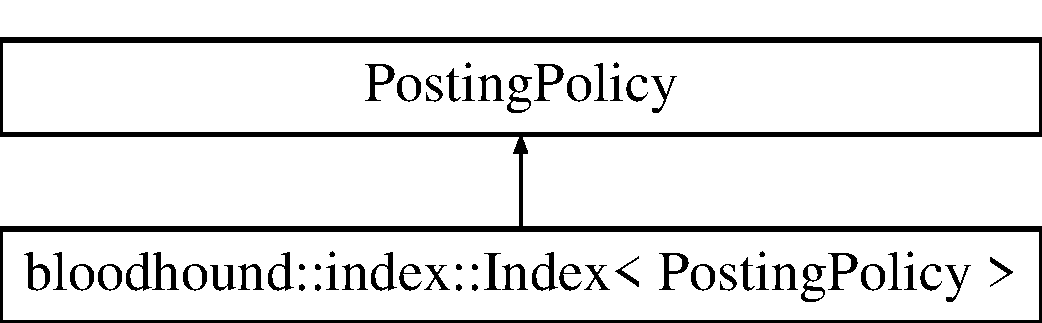
\includegraphics[height=2.000000cm]{classbloodhound_1_1index_1_1Index}
\end{center}
\end{figure}
\subsection*{Public Member Functions}
\begin{DoxyCompactItemize}
\item 
std\+::size\+\_\+t \hyperlink{classbloodhound_1_1index_1_1Index_aead1eb965d1607d25398b874cbd8a269}{get\+\_\+collection\+\_\+size} () const
\item 
\hyperlink{classbloodhound_1_1PostingList}{Posting\+List} \hyperlink{classbloodhound_1_1index_1_1Index_a24cadb41178b2cc81cf8f3e32a5dd516}{posting\+\_\+list} (\hyperlink{structbloodhound_1_1TermId}{Term\+Id} termid, bool load\+\_\+max\+\_\+scores=true)
\item 
\hyperlink{classbloodhound_1_1PostingList}{Posting\+List} \hyperlink{classbloodhound_1_1index_1_1Index_ac26271e4e2678e77d46017a24ed7eac5}{posting\+\_\+list} (\hyperlink{structbloodhound_1_1TermId}{Term\+Id} termid, double et\+\_\+threshold)
\item 
std\+::vector$<$ \hyperlink{classbloodhound_1_1PostingList}{Posting\+List} $>$ \hyperlink{classbloodhound_1_1index_1_1Index_ae36f606ee2206c44d44d0a11ae91b04c}{terms\+\_\+to\+\_\+postings} (const std\+::vector$<$ \hyperlink{structbloodhound_1_1TermId}{Term\+Id} $>$ terms)
\begin{DoxyCompactList}\small\item\em Converts a vector of terms to a vector of posting lists. \end{DoxyCompactList}\item 
void \hyperlink{classbloodhound_1_1index_1_1Index_a00eb8ae8cf8f24430fe170095c4aa4d9}{calc\+\_\+maxscores} ()
\end{DoxyCompactItemize}
\subsection*{Static Public Member Functions}
\begin{DoxyCompactItemize}
\item 
static \hyperlink{namespacebloodhound_a94032a3533df0a1b6d3435bad57e6499}{Lexicon} \hyperlink{classbloodhound_1_1index_1_1Index_a80968041cad02a4006fd4b633c279030}{load\+\_\+lexicon} (fs\+::path index\+\_\+dir)
\item 
static \hyperlink{namespacebloodhound_a687d80c6f992eba8b820bf30a482f4b4}{Max\+Scores} \hyperlink{classbloodhound_1_1index_1_1Index_a6333778f622dbf964ba6aea29a56dca0}{load\+\_\+maxscores} (fs\+::path index\+\_\+dir)
\item 
static std\+::tuple$<$ \hyperlink{namespacebloodhound_a94032a3533df0a1b6d3435bad57e6499}{Lexicon}, \hyperlink{namespacebloodhound_a687d80c6f992eba8b820bf30a482f4b4}{Max\+Scores} $>$ \hyperlink{classbloodhound_1_1index_1_1Index_a779359e7ce40294dd3d3666c00762700}{load\+\_\+mappings} (fs\+::path index\+\_\+dir)
\item 
static json\+::json \hyperlink{classbloodhound_1_1index_1_1Index_af0d9b72f7cf6b54d7bddbccd3c1898ce}{load\+\_\+meta} (fs\+::path meta\+\_\+file)
\item 
static void \hyperlink{classbloodhound_1_1index_1_1Index_a6f1e18905c2b5babd30f33467c79018a}{verify} (\hyperlink{classbloodhound_1_1index_1_1Index}{Index} \&index)
\item 
static void \hyperlink{classbloodhound_1_1index_1_1Index_a02e947bdd77e51dcb09db5b7f03f14c7}{write\+\_\+maxscores} (\hyperlink{classbloodhound_1_1index_1_1Index}{Index} \&index, fs\+::path out)
\item 
static \hyperlink{classbloodhound_1_1index_1_1Index}{Index} \hyperlink{classbloodhound_1_1index_1_1Index_a46fcfc3c54ecf18d4ff58a240557b567}{write\+\_\+maxscores} (fs\+::path index\+\_\+dir)
\item 
static \hyperlink{classbloodhound_1_1index_1_1Index}{Index} \hyperlink{classbloodhound_1_1index_1_1Index_ad4cd13bef623fc6b786f8003c8826b9c}{load\+\_\+index} (fs\+::path index\+\_\+dir, bool verify\+\_\+maxscores=false)
\end{DoxyCompactItemize}
\subsection*{Public Attributes}
\begin{DoxyCompactItemize}
\item 
\hyperlink{namespacebloodhound_a94032a3533df0a1b6d3435bad57e6499}{Lexicon} \hyperlink{classbloodhound_1_1index_1_1Index_a746d80c2fb411f512726c8d37cad78fc}{lexicon}
\end{DoxyCompactItemize}
\subsection*{Friends}
\begin{DoxyCompactItemize}
\item 
\hyperlink{classbloodhound_1_1index_1_1Index}{Index}$<$ \hyperlink{classbloodhound_1_1index_1_1InMemoryPostingPolicy}{In\+Memory\+Posting\+Policy} $>$ \hyperlink{classbloodhound_1_1index_1_1Index_a0343a97c005a2df437a955c308d376e6}{build\+\_\+index\+\_\+from\+\_\+ids} (const std\+::vector$<$ std\+::vector$<$ \hyperlink{structbloodhound_1_1TermWeight}{Term\+Weight} $>$$>$ \&input)
\item 
\hyperlink{classbloodhound_1_1index_1_1Index}{Index}$<$ \hyperlink{classbloodhound_1_1index_1_1InMemoryPostingPolicy}{In\+Memory\+Posting\+Policy} $>$ \hyperlink{classbloodhound_1_1index_1_1Index_aad81f0929f0b03479f3361a23d96573b}{sorted\+\_\+index} (const \hyperlink{classbloodhound_1_1index_1_1Index}{Index}$<$ \hyperlink{classbloodhound_1_1index_1_1InMemoryPostingPolicy}{In\+Memory\+Posting\+Policy} $>$ \&index)
\end{DoxyCompactItemize}


\subsection{Member Function Documentation}
\mbox{\Hypertarget{classbloodhound_1_1index_1_1Index_a00eb8ae8cf8f24430fe170095c4aa4d9}\label{classbloodhound_1_1index_1_1Index_a00eb8ae8cf8f24430fe170095c4aa4d9}} 
\index{bloodhound\+::index\+::\+Index@{bloodhound\+::index\+::\+Index}!calc\+\_\+maxscores@{calc\+\_\+maxscores}}
\index{calc\+\_\+maxscores@{calc\+\_\+maxscores}!bloodhound\+::index\+::\+Index@{bloodhound\+::index\+::\+Index}}
\subsubsection{\texorpdfstring{calc\+\_\+maxscores()}{calc\_maxscores()}}
{\footnotesize\ttfamily template$<$class Posting\+Policy = In\+Memory\+Posting\+Policy$>$ \\
void \hyperlink{classbloodhound_1_1index_1_1Index}{bloodhound\+::index\+::\+Index}$<$ Posting\+Policy $>$\+::calc\+\_\+maxscores (\begin{DoxyParamCaption}{ }\end{DoxyParamCaption})\hspace{0.3cm}{\ttfamily [inline]}}

\mbox{\Hypertarget{classbloodhound_1_1index_1_1Index_aead1eb965d1607d25398b874cbd8a269}\label{classbloodhound_1_1index_1_1Index_aead1eb965d1607d25398b874cbd8a269}} 
\index{bloodhound\+::index\+::\+Index@{bloodhound\+::index\+::\+Index}!get\+\_\+collection\+\_\+size@{get\+\_\+collection\+\_\+size}}
\index{get\+\_\+collection\+\_\+size@{get\+\_\+collection\+\_\+size}!bloodhound\+::index\+::\+Index@{bloodhound\+::index\+::\+Index}}
\subsubsection{\texorpdfstring{get\+\_\+collection\+\_\+size()}{get\_collection\_size()}}
{\footnotesize\ttfamily template$<$class Posting\+Policy = In\+Memory\+Posting\+Policy$>$ \\
std\+::size\+\_\+t \hyperlink{classbloodhound_1_1index_1_1Index}{bloodhound\+::index\+::\+Index}$<$ Posting\+Policy $>$\+::get\+\_\+collection\+\_\+size (\begin{DoxyParamCaption}{ }\end{DoxyParamCaption}) const\hspace{0.3cm}{\ttfamily [inline]}}

\mbox{\Hypertarget{classbloodhound_1_1index_1_1Index_ad4cd13bef623fc6b786f8003c8826b9c}\label{classbloodhound_1_1index_1_1Index_ad4cd13bef623fc6b786f8003c8826b9c}} 
\index{bloodhound\+::index\+::\+Index@{bloodhound\+::index\+::\+Index}!load\+\_\+index@{load\+\_\+index}}
\index{load\+\_\+index@{load\+\_\+index}!bloodhound\+::index\+::\+Index@{bloodhound\+::index\+::\+Index}}
\subsubsection{\texorpdfstring{load\+\_\+index()}{load\_index()}}
{\footnotesize\ttfamily template$<$class Posting\+Policy = In\+Memory\+Posting\+Policy$>$ \\
static \hyperlink{classbloodhound_1_1index_1_1Index}{Index} \hyperlink{classbloodhound_1_1index_1_1Index}{bloodhound\+::index\+::\+Index}$<$ Posting\+Policy $>$\+::load\+\_\+index (\begin{DoxyParamCaption}\item[{fs\+::path}]{index\+\_\+dir,  }\item[{bool}]{verify\+\_\+maxscores = {\ttfamily false} }\end{DoxyParamCaption})\hspace{0.3cm}{\ttfamily [inline]}, {\ttfamily [static]}}

\mbox{\Hypertarget{classbloodhound_1_1index_1_1Index_a80968041cad02a4006fd4b633c279030}\label{classbloodhound_1_1index_1_1Index_a80968041cad02a4006fd4b633c279030}} 
\index{bloodhound\+::index\+::\+Index@{bloodhound\+::index\+::\+Index}!load\+\_\+lexicon@{load\+\_\+lexicon}}
\index{load\+\_\+lexicon@{load\+\_\+lexicon}!bloodhound\+::index\+::\+Index@{bloodhound\+::index\+::\+Index}}
\subsubsection{\texorpdfstring{load\+\_\+lexicon()}{load\_lexicon()}}
{\footnotesize\ttfamily template$<$class Posting\+Policy = In\+Memory\+Posting\+Policy$>$ \\
static \hyperlink{namespacebloodhound_a94032a3533df0a1b6d3435bad57e6499}{Lexicon} \hyperlink{classbloodhound_1_1index_1_1Index}{bloodhound\+::index\+::\+Index}$<$ Posting\+Policy $>$\+::load\+\_\+lexicon (\begin{DoxyParamCaption}\item[{fs\+::path}]{index\+\_\+dir }\end{DoxyParamCaption})\hspace{0.3cm}{\ttfamily [inline]}, {\ttfamily [static]}}

\mbox{\Hypertarget{classbloodhound_1_1index_1_1Index_a779359e7ce40294dd3d3666c00762700}\label{classbloodhound_1_1index_1_1Index_a779359e7ce40294dd3d3666c00762700}} 
\index{bloodhound\+::index\+::\+Index@{bloodhound\+::index\+::\+Index}!load\+\_\+mappings@{load\+\_\+mappings}}
\index{load\+\_\+mappings@{load\+\_\+mappings}!bloodhound\+::index\+::\+Index@{bloodhound\+::index\+::\+Index}}
\subsubsection{\texorpdfstring{load\+\_\+mappings()}{load\_mappings()}}
{\footnotesize\ttfamily template$<$class Posting\+Policy = In\+Memory\+Posting\+Policy$>$ \\
static std\+::tuple$<$\hyperlink{namespacebloodhound_a94032a3533df0a1b6d3435bad57e6499}{Lexicon}, \hyperlink{namespacebloodhound_a687d80c6f992eba8b820bf30a482f4b4}{Max\+Scores}$>$ \hyperlink{classbloodhound_1_1index_1_1Index}{bloodhound\+::index\+::\+Index}$<$ Posting\+Policy $>$\+::load\+\_\+mappings (\begin{DoxyParamCaption}\item[{fs\+::path}]{index\+\_\+dir }\end{DoxyParamCaption})\hspace{0.3cm}{\ttfamily [inline]}, {\ttfamily [static]}}

\mbox{\Hypertarget{classbloodhound_1_1index_1_1Index_a6333778f622dbf964ba6aea29a56dca0}\label{classbloodhound_1_1index_1_1Index_a6333778f622dbf964ba6aea29a56dca0}} 
\index{bloodhound\+::index\+::\+Index@{bloodhound\+::index\+::\+Index}!load\+\_\+maxscores@{load\+\_\+maxscores}}
\index{load\+\_\+maxscores@{load\+\_\+maxscores}!bloodhound\+::index\+::\+Index@{bloodhound\+::index\+::\+Index}}
\subsubsection{\texorpdfstring{load\+\_\+maxscores()}{load\_maxscores()}}
{\footnotesize\ttfamily template$<$class Posting\+Policy = In\+Memory\+Posting\+Policy$>$ \\
static \hyperlink{namespacebloodhound_a687d80c6f992eba8b820bf30a482f4b4}{Max\+Scores} \hyperlink{classbloodhound_1_1index_1_1Index}{bloodhound\+::index\+::\+Index}$<$ Posting\+Policy $>$\+::load\+\_\+maxscores (\begin{DoxyParamCaption}\item[{fs\+::path}]{index\+\_\+dir }\end{DoxyParamCaption})\hspace{0.3cm}{\ttfamily [inline]}, {\ttfamily [static]}}

\mbox{\Hypertarget{classbloodhound_1_1index_1_1Index_af0d9b72f7cf6b54d7bddbccd3c1898ce}\label{classbloodhound_1_1index_1_1Index_af0d9b72f7cf6b54d7bddbccd3c1898ce}} 
\index{bloodhound\+::index\+::\+Index@{bloodhound\+::index\+::\+Index}!load\+\_\+meta@{load\+\_\+meta}}
\index{load\+\_\+meta@{load\+\_\+meta}!bloodhound\+::index\+::\+Index@{bloodhound\+::index\+::\+Index}}
\subsubsection{\texorpdfstring{load\+\_\+meta()}{load\_meta()}}
{\footnotesize\ttfamily template$<$class Posting\+Policy = In\+Memory\+Posting\+Policy$>$ \\
static json\+::json \hyperlink{classbloodhound_1_1index_1_1Index}{bloodhound\+::index\+::\+Index}$<$ Posting\+Policy $>$\+::load\+\_\+meta (\begin{DoxyParamCaption}\item[{fs\+::path}]{meta\+\_\+file }\end{DoxyParamCaption})\hspace{0.3cm}{\ttfamily [inline]}, {\ttfamily [static]}}

\mbox{\Hypertarget{classbloodhound_1_1index_1_1Index_a24cadb41178b2cc81cf8f3e32a5dd516}\label{classbloodhound_1_1index_1_1Index_a24cadb41178b2cc81cf8f3e32a5dd516}} 
\index{bloodhound\+::index\+::\+Index@{bloodhound\+::index\+::\+Index}!posting\+\_\+list@{posting\+\_\+list}}
\index{posting\+\_\+list@{posting\+\_\+list}!bloodhound\+::index\+::\+Index@{bloodhound\+::index\+::\+Index}}
\subsubsection{\texorpdfstring{posting\+\_\+list()}{posting\_list()}\hspace{0.1cm}{\footnotesize\ttfamily [1/2]}}
{\footnotesize\ttfamily template$<$class Posting\+Policy = In\+Memory\+Posting\+Policy$>$ \\
\hyperlink{classbloodhound_1_1PostingList}{Posting\+List} \hyperlink{classbloodhound_1_1index_1_1Index}{bloodhound\+::index\+::\+Index}$<$ Posting\+Policy $>$\+::posting\+\_\+list (\begin{DoxyParamCaption}\item[{\hyperlink{structbloodhound_1_1TermId}{Term\+Id}}]{termid,  }\item[{bool}]{load\+\_\+max\+\_\+scores = {\ttfamily true} }\end{DoxyParamCaption})\hspace{0.3cm}{\ttfamily [inline]}}

\mbox{\Hypertarget{classbloodhound_1_1index_1_1Index_ac26271e4e2678e77d46017a24ed7eac5}\label{classbloodhound_1_1index_1_1Index_ac26271e4e2678e77d46017a24ed7eac5}} 
\index{bloodhound\+::index\+::\+Index@{bloodhound\+::index\+::\+Index}!posting\+\_\+list@{posting\+\_\+list}}
\index{posting\+\_\+list@{posting\+\_\+list}!bloodhound\+::index\+::\+Index@{bloodhound\+::index\+::\+Index}}
\subsubsection{\texorpdfstring{posting\+\_\+list()}{posting\_list()}\hspace{0.1cm}{\footnotesize\ttfamily [2/2]}}
{\footnotesize\ttfamily template$<$class Posting\+Policy = In\+Memory\+Posting\+Policy$>$ \\
\hyperlink{classbloodhound_1_1PostingList}{Posting\+List} \hyperlink{classbloodhound_1_1index_1_1Index}{bloodhound\+::index\+::\+Index}$<$ Posting\+Policy $>$\+::posting\+\_\+list (\begin{DoxyParamCaption}\item[{\hyperlink{structbloodhound_1_1TermId}{Term\+Id}}]{termid,  }\item[{double}]{et\+\_\+threshold }\end{DoxyParamCaption})\hspace{0.3cm}{\ttfamily [inline]}}

\mbox{\Hypertarget{classbloodhound_1_1index_1_1Index_ae36f606ee2206c44d44d0a11ae91b04c}\label{classbloodhound_1_1index_1_1Index_ae36f606ee2206c44d44d0a11ae91b04c}} 
\index{bloodhound\+::index\+::\+Index@{bloodhound\+::index\+::\+Index}!terms\+\_\+to\+\_\+postings@{terms\+\_\+to\+\_\+postings}}
\index{terms\+\_\+to\+\_\+postings@{terms\+\_\+to\+\_\+postings}!bloodhound\+::index\+::\+Index@{bloodhound\+::index\+::\+Index}}
\subsubsection{\texorpdfstring{terms\+\_\+to\+\_\+postings()}{terms\_to\_postings()}}
{\footnotesize\ttfamily template$<$class Posting\+Policy = In\+Memory\+Posting\+Policy$>$ \\
std\+::vector$<$\hyperlink{classbloodhound_1_1PostingList}{Posting\+List}$>$ \hyperlink{classbloodhound_1_1index_1_1Index}{bloodhound\+::index\+::\+Index}$<$ Posting\+Policy $>$\+::terms\+\_\+to\+\_\+postings (\begin{DoxyParamCaption}\item[{const std\+::vector$<$ \hyperlink{structbloodhound_1_1TermId}{Term\+Id} $>$}]{terms }\end{DoxyParamCaption})\hspace{0.3cm}{\ttfamily [inline]}}



Converts a vector of terms to a vector of posting lists. 

\mbox{\Hypertarget{classbloodhound_1_1index_1_1Index_a6f1e18905c2b5babd30f33467c79018a}\label{classbloodhound_1_1index_1_1Index_a6f1e18905c2b5babd30f33467c79018a}} 
\index{bloodhound\+::index\+::\+Index@{bloodhound\+::index\+::\+Index}!verify@{verify}}
\index{verify@{verify}!bloodhound\+::index\+::\+Index@{bloodhound\+::index\+::\+Index}}
\subsubsection{\texorpdfstring{verify()}{verify()}}
{\footnotesize\ttfamily template$<$class Posting\+Policy = In\+Memory\+Posting\+Policy$>$ \\
static void \hyperlink{classbloodhound_1_1index_1_1Index}{bloodhound\+::index\+::\+Index}$<$ Posting\+Policy $>$\+::verify (\begin{DoxyParamCaption}\item[{\hyperlink{classbloodhound_1_1index_1_1Index}{Index}$<$ Posting\+Policy $>$ \&}]{index }\end{DoxyParamCaption})\hspace{0.3cm}{\ttfamily [inline]}, {\ttfamily [static]}}

\mbox{\Hypertarget{classbloodhound_1_1index_1_1Index_a02e947bdd77e51dcb09db5b7f03f14c7}\label{classbloodhound_1_1index_1_1Index_a02e947bdd77e51dcb09db5b7f03f14c7}} 
\index{bloodhound\+::index\+::\+Index@{bloodhound\+::index\+::\+Index}!write\+\_\+maxscores@{write\+\_\+maxscores}}
\index{write\+\_\+maxscores@{write\+\_\+maxscores}!bloodhound\+::index\+::\+Index@{bloodhound\+::index\+::\+Index}}
\subsubsection{\texorpdfstring{write\+\_\+maxscores()}{write\_maxscores()}\hspace{0.1cm}{\footnotesize\ttfamily [1/2]}}
{\footnotesize\ttfamily template$<$class Posting\+Policy = In\+Memory\+Posting\+Policy$>$ \\
static void \hyperlink{classbloodhound_1_1index_1_1Index}{bloodhound\+::index\+::\+Index}$<$ Posting\+Policy $>$\+::write\+\_\+maxscores (\begin{DoxyParamCaption}\item[{\hyperlink{classbloodhound_1_1index_1_1Index}{Index}$<$ Posting\+Policy $>$ \&}]{index,  }\item[{fs\+::path}]{out }\end{DoxyParamCaption})\hspace{0.3cm}{\ttfamily [inline]}, {\ttfamily [static]}}

\mbox{\Hypertarget{classbloodhound_1_1index_1_1Index_a46fcfc3c54ecf18d4ff58a240557b567}\label{classbloodhound_1_1index_1_1Index_a46fcfc3c54ecf18d4ff58a240557b567}} 
\index{bloodhound\+::index\+::\+Index@{bloodhound\+::index\+::\+Index}!write\+\_\+maxscores@{write\+\_\+maxscores}}
\index{write\+\_\+maxscores@{write\+\_\+maxscores}!bloodhound\+::index\+::\+Index@{bloodhound\+::index\+::\+Index}}
\subsubsection{\texorpdfstring{write\+\_\+maxscores()}{write\_maxscores()}\hspace{0.1cm}{\footnotesize\ttfamily [2/2]}}
{\footnotesize\ttfamily template$<$class Posting\+Policy = In\+Memory\+Posting\+Policy$>$ \\
static \hyperlink{classbloodhound_1_1index_1_1Index}{Index} \hyperlink{classbloodhound_1_1index_1_1Index}{bloodhound\+::index\+::\+Index}$<$ Posting\+Policy $>$\+::write\+\_\+maxscores (\begin{DoxyParamCaption}\item[{fs\+::path}]{index\+\_\+dir }\end{DoxyParamCaption})\hspace{0.3cm}{\ttfamily [inline]}, {\ttfamily [static]}}



\subsection{Friends And Related Function Documentation}
\mbox{\Hypertarget{classbloodhound_1_1index_1_1Index_a0343a97c005a2df437a955c308d376e6}\label{classbloodhound_1_1index_1_1Index_a0343a97c005a2df437a955c308d376e6}} 
\index{bloodhound\+::index\+::\+Index@{bloodhound\+::index\+::\+Index}!build\+\_\+index\+\_\+from\+\_\+ids@{build\+\_\+index\+\_\+from\+\_\+ids}}
\index{build\+\_\+index\+\_\+from\+\_\+ids@{build\+\_\+index\+\_\+from\+\_\+ids}!bloodhound\+::index\+::\+Index@{bloodhound\+::index\+::\+Index}}
\subsubsection{\texorpdfstring{build\+\_\+index\+\_\+from\+\_\+ids}{build\_index\_from\_ids}}
{\footnotesize\ttfamily template$<$class Posting\+Policy = In\+Memory\+Posting\+Policy$>$ \\
\hyperlink{classbloodhound_1_1index_1_1Index}{Index}$<$\hyperlink{classbloodhound_1_1index_1_1InMemoryPostingPolicy}{In\+Memory\+Posting\+Policy}$>$ build\+\_\+index\+\_\+from\+\_\+ids (\begin{DoxyParamCaption}\item[{const std\+::vector$<$ std\+::vector$<$ \hyperlink{structbloodhound_1_1TermWeight}{Term\+Weight} $>$$>$ \&}]{input }\end{DoxyParamCaption})\hspace{0.3cm}{\ttfamily [friend]}}

Builds an index based on a collection represented by term I\+Ds.

This function is not efficient and only meant for testing other functionalities. \mbox{\Hypertarget{classbloodhound_1_1index_1_1Index_aad81f0929f0b03479f3361a23d96573b}\label{classbloodhound_1_1index_1_1Index_aad81f0929f0b03479f3361a23d96573b}} 
\index{bloodhound\+::index\+::\+Index@{bloodhound\+::index\+::\+Index}!sorted\+\_\+index@{sorted\+\_\+index}}
\index{sorted\+\_\+index@{sorted\+\_\+index}!bloodhound\+::index\+::\+Index@{bloodhound\+::index\+::\+Index}}
\subsubsection{\texorpdfstring{sorted\+\_\+index}{sorted\_index}}
{\footnotesize\ttfamily template$<$class Posting\+Policy = In\+Memory\+Posting\+Policy$>$ \\
\hyperlink{classbloodhound_1_1index_1_1Index}{Index}$<$\hyperlink{classbloodhound_1_1index_1_1InMemoryPostingPolicy}{In\+Memory\+Posting\+Policy}$>$ sorted\+\_\+index (\begin{DoxyParamCaption}\item[{const \hyperlink{classbloodhound_1_1index_1_1Index}{Index}$<$ \hyperlink{classbloodhound_1_1index_1_1InMemoryPostingPolicy}{In\+Memory\+Posting\+Policy} $>$ \&}]{index }\end{DoxyParamCaption})\hspace{0.3cm}{\ttfamily [friend]}}



\subsection{Member Data Documentation}
\mbox{\Hypertarget{classbloodhound_1_1index_1_1Index_a746d80c2fb411f512726c8d37cad78fc}\label{classbloodhound_1_1index_1_1Index_a746d80c2fb411f512726c8d37cad78fc}} 
\index{bloodhound\+::index\+::\+Index@{bloodhound\+::index\+::\+Index}!lexicon@{lexicon}}
\index{lexicon@{lexicon}!bloodhound\+::index\+::\+Index@{bloodhound\+::index\+::\+Index}}
\subsubsection{\texorpdfstring{lexicon}{lexicon}}
{\footnotesize\ttfamily template$<$class Posting\+Policy = In\+Memory\+Posting\+Policy$>$ \\
\hyperlink{namespacebloodhound_a94032a3533df0a1b6d3435bad57e6499}{Lexicon} \hyperlink{classbloodhound_1_1index_1_1Index}{bloodhound\+::index\+::\+Index}$<$ Posting\+Policy $>$\+::lexicon}



The documentation for this class was generated from the following file\+:\begin{DoxyCompactItemize}
\item 
include/\hyperlink{index_8hpp}{index.\+hpp}\end{DoxyCompactItemize}

\hypertarget{classbloodhound_1_1index_1_1InMemoryPostingPolicy}{}\section{bloodhound\+:\+:index\+:\+:In\+Memory\+Posting\+Policy Class Reference}
\label{classbloodhound_1_1index_1_1InMemoryPostingPolicy}\index{bloodhound\+::index\+::\+In\+Memory\+Posting\+Policy@{bloodhound\+::index\+::\+In\+Memory\+Posting\+Policy}}


{\ttfamily \#include $<$index.\+hpp$>$}

\subsection*{Protected Member Functions}
\begin{DoxyCompactItemize}
\item 
char $\ast$ \hyperlink{classbloodhound_1_1index_1_1InMemoryPostingPolicy_acc5567fd6ba17861290ba045567e7e1a}{read\+\_\+posting\+\_\+data} (\hyperlink{structbloodhound_1_1Offset}{Offset} offset)
\item 
void \hyperlink{classbloodhound_1_1index_1_1InMemoryPostingPolicy_a68a2a76f7b4349ade63f83acfd6a1dc5}{load\+\_\+postings} (fs\+::path postings\+\_\+file)
\end{DoxyCompactItemize}
\subsection*{Protected Attributes}
\begin{DoxyCompactItemize}
\item 
std\+::vector$<$ char $>$ \hyperlink{classbloodhound_1_1index_1_1InMemoryPostingPolicy_ae760569f621a8b6260cbc50c144be0bf}{postings\+\_\+data}
\end{DoxyCompactItemize}


\subsection{Member Function Documentation}
\mbox{\Hypertarget{classbloodhound_1_1index_1_1InMemoryPostingPolicy_a68a2a76f7b4349ade63f83acfd6a1dc5}\label{classbloodhound_1_1index_1_1InMemoryPostingPolicy_a68a2a76f7b4349ade63f83acfd6a1dc5}} 
\index{bloodhound\+::index\+::\+In\+Memory\+Posting\+Policy@{bloodhound\+::index\+::\+In\+Memory\+Posting\+Policy}!load\+\_\+postings@{load\+\_\+postings}}
\index{load\+\_\+postings@{load\+\_\+postings}!bloodhound\+::index\+::\+In\+Memory\+Posting\+Policy@{bloodhound\+::index\+::\+In\+Memory\+Posting\+Policy}}
\subsubsection{\texorpdfstring{load\+\_\+postings()}{load\_postings()}}
{\footnotesize\ttfamily void bloodhound\+::index\+::\+In\+Memory\+Posting\+Policy\+::load\+\_\+postings (\begin{DoxyParamCaption}\item[{fs\+::path}]{postings\+\_\+file }\end{DoxyParamCaption})\hspace{0.3cm}{\ttfamily [inline]}, {\ttfamily [protected]}}

\mbox{\Hypertarget{classbloodhound_1_1index_1_1InMemoryPostingPolicy_acc5567fd6ba17861290ba045567e7e1a}\label{classbloodhound_1_1index_1_1InMemoryPostingPolicy_acc5567fd6ba17861290ba045567e7e1a}} 
\index{bloodhound\+::index\+::\+In\+Memory\+Posting\+Policy@{bloodhound\+::index\+::\+In\+Memory\+Posting\+Policy}!read\+\_\+posting\+\_\+data@{read\+\_\+posting\+\_\+data}}
\index{read\+\_\+posting\+\_\+data@{read\+\_\+posting\+\_\+data}!bloodhound\+::index\+::\+In\+Memory\+Posting\+Policy@{bloodhound\+::index\+::\+In\+Memory\+Posting\+Policy}}
\subsubsection{\texorpdfstring{read\+\_\+posting\+\_\+data()}{read\_posting\_data()}}
{\footnotesize\ttfamily char$\ast$ bloodhound\+::index\+::\+In\+Memory\+Posting\+Policy\+::read\+\_\+posting\+\_\+data (\begin{DoxyParamCaption}\item[{\hyperlink{structbloodhound_1_1Offset}{Offset}}]{offset }\end{DoxyParamCaption})\hspace{0.3cm}{\ttfamily [inline]}, {\ttfamily [protected]}}



\subsection{Member Data Documentation}
\mbox{\Hypertarget{classbloodhound_1_1index_1_1InMemoryPostingPolicy_ae760569f621a8b6260cbc50c144be0bf}\label{classbloodhound_1_1index_1_1InMemoryPostingPolicy_ae760569f621a8b6260cbc50c144be0bf}} 
\index{bloodhound\+::index\+::\+In\+Memory\+Posting\+Policy@{bloodhound\+::index\+::\+In\+Memory\+Posting\+Policy}!postings\+\_\+data@{postings\+\_\+data}}
\index{postings\+\_\+data@{postings\+\_\+data}!bloodhound\+::index\+::\+In\+Memory\+Posting\+Policy@{bloodhound\+::index\+::\+In\+Memory\+Posting\+Policy}}
\subsubsection{\texorpdfstring{postings\+\_\+data}{postings\_data}}
{\footnotesize\ttfamily std\+::vector$<$char$>$ bloodhound\+::index\+::\+In\+Memory\+Posting\+Policy\+::postings\+\_\+data\hspace{0.3cm}{\ttfamily [protected]}}



The documentation for this class was generated from the following file\+:\begin{DoxyCompactItemize}
\item 
include/\hyperlink{index_8hpp}{index.\+hpp}\end{DoxyCompactItemize}

\hypertarget{structbloodhound_1_1PostingList_1_1iterator}{}\section{bloodhound\+:\+:Posting\+List\+:\+:iterator Struct Reference}
\label{structbloodhound_1_1PostingList_1_1iterator}\index{bloodhound\+::\+Posting\+List\+::iterator@{bloodhound\+::\+Posting\+List\+::iterator}}


{\ttfamily \#include $<$index.\+hpp$>$}

\subsection*{Public Member Functions}
\begin{DoxyCompactItemize}
\item 
\mbox{\hyperlink{structbloodhound_1_1PostingList_1_1iterator_af815248890d1f92dbd2cc3fa5813875a}{iterator}} (const \mbox{\hyperlink{classbloodhound_1_1PostingList}{Posting\+List}} $\ast$pl, std\+::size\+\_\+t p)
\item 
\mbox{\hyperlink{structbloodhound_1_1Posting}{Posting}} \& \mbox{\hyperlink{structbloodhound_1_1PostingList_1_1iterator_a386a2af6b962ddd85392f1313eb16eff}{operator$\ast$}} ()
\item 
\mbox{\hyperlink{structbloodhound_1_1Posting}{Posting}} $\ast$ \mbox{\hyperlink{structbloodhound_1_1PostingList_1_1iterator_a8c9120139692d6672b52d96301718614}{operator-\/$>$}} ()
\item 
\mbox{\hyperlink{structbloodhound_1_1PostingList_1_1iterator}{iterator}} \& \mbox{\hyperlink{structbloodhound_1_1PostingList_1_1iterator_a8b0c2e4221f0ce3ea893c2fc37edbd53}{operator++}} ()
\item 
\mbox{\hyperlink{structbloodhound_1_1PostingList_1_1iterator}{iterator}} \mbox{\hyperlink{structbloodhound_1_1PostingList_1_1iterator_a9923c5a81b77562a06a48562babcdc9b}{operator++}} (int)
\item 
\mbox{\hyperlink{structbloodhound_1_1PostingList_1_1iterator}{iterator}} \mbox{\hyperlink{structbloodhound_1_1PostingList_1_1iterator_a8672fb454e60ed068ae02078976543f9}{operator+}} (int n) const
\item 
\mbox{\hyperlink{structbloodhound_1_1PostingList_1_1iterator}{iterator}} \mbox{\hyperlink{structbloodhound_1_1PostingList_1_1iterator_a61a5de181ff84ddc0976957a7a9fcfd7}{operator-\/}} (int n) const
\item 
bool \mbox{\hyperlink{structbloodhound_1_1PostingList_1_1iterator_af82060f61f9231ee449e43ea347cab29}{operator==}} (\mbox{\hyperlink{structbloodhound_1_1PostingList_1_1iterator}{iterator}} rhs) const
\item 
bool \mbox{\hyperlink{structbloodhound_1_1PostingList_1_1iterator_aa293b4e0607edaca2fde163c8ee0f00e}{operator!=}} (\mbox{\hyperlink{structbloodhound_1_1PostingList_1_1iterator}{iterator}} rhs) const
\item 
\mbox{\hyperlink{structbloodhound_1_1Doc}{Doc}} \mbox{\hyperlink{structbloodhound_1_1PostingList_1_1iterator_a995d206215c6a01d7a183666502e2628}{doc}} ()
\item 
\mbox{\hyperlink{structbloodhound_1_1Score}{Score}} \mbox{\hyperlink{structbloodhound_1_1PostingList_1_1iterator_a5c94dca7f430ac78f0db3f0fe2c01c75}{score}} ()
\end{DoxyCompactItemize}
\subsection*{Public Attributes}
\begin{DoxyCompactItemize}
\item 
const \mbox{\hyperlink{classbloodhound_1_1PostingList}{Posting\+List}} $\ast$ \mbox{\hyperlink{structbloodhound_1_1PostingList_1_1iterator_a3a9afedb85f883831ee68fee0611ca92}{posting\+\_\+list}}
\item 
std\+::size\+\_\+t \mbox{\hyperlink{structbloodhound_1_1PostingList_1_1iterator_a544fdd6020d2ec35d883250dd79115e8}{pos}}
\item 
\mbox{\hyperlink{structbloodhound_1_1Posting}{Posting}} \mbox{\hyperlink{structbloodhound_1_1PostingList_1_1iterator_ae4e6a0f32f80ac9f64558843a0a0cf0e}{current}}
\end{DoxyCompactItemize}


\subsection{Constructor \& Destructor Documentation}
\mbox{\Hypertarget{structbloodhound_1_1PostingList_1_1iterator_af815248890d1f92dbd2cc3fa5813875a}\label{structbloodhound_1_1PostingList_1_1iterator_af815248890d1f92dbd2cc3fa5813875a}} 
\index{bloodhound\+::\+Posting\+List\+::iterator@{bloodhound\+::\+Posting\+List\+::iterator}!iterator@{iterator}}
\index{iterator@{iterator}!bloodhound\+::\+Posting\+List\+::iterator@{bloodhound\+::\+Posting\+List\+::iterator}}
\subsubsection{\texorpdfstring{iterator()}{iterator()}}
{\footnotesize\ttfamily bloodhound\+::\+Posting\+List\+::iterator\+::iterator (\begin{DoxyParamCaption}\item[{const \mbox{\hyperlink{classbloodhound_1_1PostingList}{Posting\+List}} $\ast$}]{pl,  }\item[{std\+::size\+\_\+t}]{p }\end{DoxyParamCaption})\hspace{0.3cm}{\ttfamily [inline]}}



\subsection{Member Function Documentation}
\mbox{\Hypertarget{structbloodhound_1_1PostingList_1_1iterator_a995d206215c6a01d7a183666502e2628}\label{structbloodhound_1_1PostingList_1_1iterator_a995d206215c6a01d7a183666502e2628}} 
\index{bloodhound\+::\+Posting\+List\+::iterator@{bloodhound\+::\+Posting\+List\+::iterator}!doc@{doc}}
\index{doc@{doc}!bloodhound\+::\+Posting\+List\+::iterator@{bloodhound\+::\+Posting\+List\+::iterator}}
\subsubsection{\texorpdfstring{doc()}{doc()}}
{\footnotesize\ttfamily \mbox{\hyperlink{structbloodhound_1_1Doc}{Doc}} bloodhound\+::\+Posting\+List\+::iterator\+::doc (\begin{DoxyParamCaption}{ }\end{DoxyParamCaption})\hspace{0.3cm}{\ttfamily [inline]}}

\mbox{\Hypertarget{structbloodhound_1_1PostingList_1_1iterator_aa293b4e0607edaca2fde163c8ee0f00e}\label{structbloodhound_1_1PostingList_1_1iterator_aa293b4e0607edaca2fde163c8ee0f00e}} 
\index{bloodhound\+::\+Posting\+List\+::iterator@{bloodhound\+::\+Posting\+List\+::iterator}!operator"!=@{operator"!=}}
\index{operator"!=@{operator"!=}!bloodhound\+::\+Posting\+List\+::iterator@{bloodhound\+::\+Posting\+List\+::iterator}}
\subsubsection{\texorpdfstring{operator"!=()}{operator!=()}}
{\footnotesize\ttfamily bool bloodhound\+::\+Posting\+List\+::iterator\+::operator!= (\begin{DoxyParamCaption}\item[{\mbox{\hyperlink{structbloodhound_1_1PostingList_1_1iterator}{iterator}}}]{rhs }\end{DoxyParamCaption}) const\hspace{0.3cm}{\ttfamily [inline]}}

\mbox{\Hypertarget{structbloodhound_1_1PostingList_1_1iterator_a386a2af6b962ddd85392f1313eb16eff}\label{structbloodhound_1_1PostingList_1_1iterator_a386a2af6b962ddd85392f1313eb16eff}} 
\index{bloodhound\+::\+Posting\+List\+::iterator@{bloodhound\+::\+Posting\+List\+::iterator}!operator$\ast$@{operator$\ast$}}
\index{operator$\ast$@{operator$\ast$}!bloodhound\+::\+Posting\+List\+::iterator@{bloodhound\+::\+Posting\+List\+::iterator}}
\subsubsection{\texorpdfstring{operator$\ast$()}{operator*()}}
{\footnotesize\ttfamily \mbox{\hyperlink{structbloodhound_1_1Posting}{Posting}}\& bloodhound\+::\+Posting\+List\+::iterator\+::operator$\ast$ (\begin{DoxyParamCaption}{ }\end{DoxyParamCaption})\hspace{0.3cm}{\ttfamily [inline]}}

\mbox{\Hypertarget{structbloodhound_1_1PostingList_1_1iterator_a8672fb454e60ed068ae02078976543f9}\label{structbloodhound_1_1PostingList_1_1iterator_a8672fb454e60ed068ae02078976543f9}} 
\index{bloodhound\+::\+Posting\+List\+::iterator@{bloodhound\+::\+Posting\+List\+::iterator}!operator+@{operator+}}
\index{operator+@{operator+}!bloodhound\+::\+Posting\+List\+::iterator@{bloodhound\+::\+Posting\+List\+::iterator}}
\subsubsection{\texorpdfstring{operator+()}{operator+()}}
{\footnotesize\ttfamily \mbox{\hyperlink{structbloodhound_1_1PostingList_1_1iterator}{iterator}} bloodhound\+::\+Posting\+List\+::iterator\+::operator+ (\begin{DoxyParamCaption}\item[{int}]{n }\end{DoxyParamCaption}) const\hspace{0.3cm}{\ttfamily [inline]}}

\mbox{\Hypertarget{structbloodhound_1_1PostingList_1_1iterator_a8b0c2e4221f0ce3ea893c2fc37edbd53}\label{structbloodhound_1_1PostingList_1_1iterator_a8b0c2e4221f0ce3ea893c2fc37edbd53}} 
\index{bloodhound\+::\+Posting\+List\+::iterator@{bloodhound\+::\+Posting\+List\+::iterator}!operator++@{operator++}}
\index{operator++@{operator++}!bloodhound\+::\+Posting\+List\+::iterator@{bloodhound\+::\+Posting\+List\+::iterator}}
\subsubsection{\texorpdfstring{operator++()}{operator++()}\hspace{0.1cm}{\footnotesize\ttfamily [1/2]}}
{\footnotesize\ttfamily \mbox{\hyperlink{structbloodhound_1_1PostingList_1_1iterator}{iterator}}\& bloodhound\+::\+Posting\+List\+::iterator\+::operator++ (\begin{DoxyParamCaption}{ }\end{DoxyParamCaption})\hspace{0.3cm}{\ttfamily [inline]}}

\mbox{\Hypertarget{structbloodhound_1_1PostingList_1_1iterator_a9923c5a81b77562a06a48562babcdc9b}\label{structbloodhound_1_1PostingList_1_1iterator_a9923c5a81b77562a06a48562babcdc9b}} 
\index{bloodhound\+::\+Posting\+List\+::iterator@{bloodhound\+::\+Posting\+List\+::iterator}!operator++@{operator++}}
\index{operator++@{operator++}!bloodhound\+::\+Posting\+List\+::iterator@{bloodhound\+::\+Posting\+List\+::iterator}}
\subsubsection{\texorpdfstring{operator++()}{operator++()}\hspace{0.1cm}{\footnotesize\ttfamily [2/2]}}
{\footnotesize\ttfamily \mbox{\hyperlink{structbloodhound_1_1PostingList_1_1iterator}{iterator}} bloodhound\+::\+Posting\+List\+::iterator\+::operator++ (\begin{DoxyParamCaption}\item[{int}]{ }\end{DoxyParamCaption})\hspace{0.3cm}{\ttfamily [inline]}}

\mbox{\Hypertarget{structbloodhound_1_1PostingList_1_1iterator_a61a5de181ff84ddc0976957a7a9fcfd7}\label{structbloodhound_1_1PostingList_1_1iterator_a61a5de181ff84ddc0976957a7a9fcfd7}} 
\index{bloodhound\+::\+Posting\+List\+::iterator@{bloodhound\+::\+Posting\+List\+::iterator}!operator-\/@{operator-\/}}
\index{operator-\/@{operator-\/}!bloodhound\+::\+Posting\+List\+::iterator@{bloodhound\+::\+Posting\+List\+::iterator}}
\subsubsection{\texorpdfstring{operator-\/()}{operator-()}}
{\footnotesize\ttfamily \mbox{\hyperlink{structbloodhound_1_1PostingList_1_1iterator}{iterator}} bloodhound\+::\+Posting\+List\+::iterator\+::operator-\/ (\begin{DoxyParamCaption}\item[{int}]{n }\end{DoxyParamCaption}) const\hspace{0.3cm}{\ttfamily [inline]}}

\mbox{\Hypertarget{structbloodhound_1_1PostingList_1_1iterator_a8c9120139692d6672b52d96301718614}\label{structbloodhound_1_1PostingList_1_1iterator_a8c9120139692d6672b52d96301718614}} 
\index{bloodhound\+::\+Posting\+List\+::iterator@{bloodhound\+::\+Posting\+List\+::iterator}!operator-\/$>$@{operator-\/$>$}}
\index{operator-\/$>$@{operator-\/$>$}!bloodhound\+::\+Posting\+List\+::iterator@{bloodhound\+::\+Posting\+List\+::iterator}}
\subsubsection{\texorpdfstring{operator-\/$>$()}{operator->()}}
{\footnotesize\ttfamily \mbox{\hyperlink{structbloodhound_1_1Posting}{Posting}}$\ast$ bloodhound\+::\+Posting\+List\+::iterator\+::operator-\/$>$ (\begin{DoxyParamCaption}{ }\end{DoxyParamCaption})\hspace{0.3cm}{\ttfamily [inline]}}

\mbox{\Hypertarget{structbloodhound_1_1PostingList_1_1iterator_af82060f61f9231ee449e43ea347cab29}\label{structbloodhound_1_1PostingList_1_1iterator_af82060f61f9231ee449e43ea347cab29}} 
\index{bloodhound\+::\+Posting\+List\+::iterator@{bloodhound\+::\+Posting\+List\+::iterator}!operator==@{operator==}}
\index{operator==@{operator==}!bloodhound\+::\+Posting\+List\+::iterator@{bloodhound\+::\+Posting\+List\+::iterator}}
\subsubsection{\texorpdfstring{operator==()}{operator==()}}
{\footnotesize\ttfamily bool bloodhound\+::\+Posting\+List\+::iterator\+::operator== (\begin{DoxyParamCaption}\item[{\mbox{\hyperlink{structbloodhound_1_1PostingList_1_1iterator}{iterator}}}]{rhs }\end{DoxyParamCaption}) const\hspace{0.3cm}{\ttfamily [inline]}}

\mbox{\Hypertarget{structbloodhound_1_1PostingList_1_1iterator_a5c94dca7f430ac78f0db3f0fe2c01c75}\label{structbloodhound_1_1PostingList_1_1iterator_a5c94dca7f430ac78f0db3f0fe2c01c75}} 
\index{bloodhound\+::\+Posting\+List\+::iterator@{bloodhound\+::\+Posting\+List\+::iterator}!score@{score}}
\index{score@{score}!bloodhound\+::\+Posting\+List\+::iterator@{bloodhound\+::\+Posting\+List\+::iterator}}
\subsubsection{\texorpdfstring{score()}{score()}}
{\footnotesize\ttfamily \mbox{\hyperlink{structbloodhound_1_1Score}{Score}} bloodhound\+::\+Posting\+List\+::iterator\+::score (\begin{DoxyParamCaption}{ }\end{DoxyParamCaption})\hspace{0.3cm}{\ttfamily [inline]}}



\subsection{Member Data Documentation}
\mbox{\Hypertarget{structbloodhound_1_1PostingList_1_1iterator_ae4e6a0f32f80ac9f64558843a0a0cf0e}\label{structbloodhound_1_1PostingList_1_1iterator_ae4e6a0f32f80ac9f64558843a0a0cf0e}} 
\index{bloodhound\+::\+Posting\+List\+::iterator@{bloodhound\+::\+Posting\+List\+::iterator}!current@{current}}
\index{current@{current}!bloodhound\+::\+Posting\+List\+::iterator@{bloodhound\+::\+Posting\+List\+::iterator}}
\subsubsection{\texorpdfstring{current}{current}}
{\footnotesize\ttfamily \mbox{\hyperlink{structbloodhound_1_1Posting}{Posting}} bloodhound\+::\+Posting\+List\+::iterator\+::current}

\mbox{\Hypertarget{structbloodhound_1_1PostingList_1_1iterator_a544fdd6020d2ec35d883250dd79115e8}\label{structbloodhound_1_1PostingList_1_1iterator_a544fdd6020d2ec35d883250dd79115e8}} 
\index{bloodhound\+::\+Posting\+List\+::iterator@{bloodhound\+::\+Posting\+List\+::iterator}!pos@{pos}}
\index{pos@{pos}!bloodhound\+::\+Posting\+List\+::iterator@{bloodhound\+::\+Posting\+List\+::iterator}}
\subsubsection{\texorpdfstring{pos}{pos}}
{\footnotesize\ttfamily std\+::size\+\_\+t bloodhound\+::\+Posting\+List\+::iterator\+::pos}

\mbox{\Hypertarget{structbloodhound_1_1PostingList_1_1iterator_a3a9afedb85f883831ee68fee0611ca92}\label{structbloodhound_1_1PostingList_1_1iterator_a3a9afedb85f883831ee68fee0611ca92}} 
\index{bloodhound\+::\+Posting\+List\+::iterator@{bloodhound\+::\+Posting\+List\+::iterator}!posting\+\_\+list@{posting\+\_\+list}}
\index{posting\+\_\+list@{posting\+\_\+list}!bloodhound\+::\+Posting\+List\+::iterator@{bloodhound\+::\+Posting\+List\+::iterator}}
\subsubsection{\texorpdfstring{posting\+\_\+list}{posting\_list}}
{\footnotesize\ttfamily const \mbox{\hyperlink{classbloodhound_1_1PostingList}{Posting\+List}}$\ast$ bloodhound\+::\+Posting\+List\+::iterator\+::posting\+\_\+list}



The documentation for this struct was generated from the following file\+:\begin{DoxyCompactItemize}
\item 
include/\mbox{\hyperlink{index_8hpp}{index.\+hpp}}\end{DoxyCompactItemize}

\hypertarget{structbloodhound_1_1query_1_1DaatRetriever_1_1IteratorPair}{}\section{bloodhound\+:\+:query\+:\+:Daat\+Retriever$<$ Posting\+List $>$\+:\+:Iterator\+Pair Struct Reference}
\label{structbloodhound_1_1query_1_1DaatRetriever_1_1IteratorPair}\index{bloodhound\+::query\+::\+Daat\+Retriever$<$ Posting\+List $>$\+::\+Iterator\+Pair@{bloodhound\+::query\+::\+Daat\+Retriever$<$ Posting\+List $>$\+::\+Iterator\+Pair}}


Current and end iterators of the same posting list.  




{\ttfamily \#include $<$retrievers.\+hpp$>$}

\subsection*{Public Attributes}
\begin{DoxyCompactItemize}
\item 
\hyperlink{structbloodhound_1_1PostingList_1_1iterator}{Posting\+List\+::iterator} \hyperlink{structbloodhound_1_1query_1_1DaatRetriever_1_1IteratorPair_a39776930389d36b2b0da49c3b5685ec4}{current}
\item 
\hyperlink{structbloodhound_1_1PostingList_1_1iterator}{Posting\+List\+::iterator} \hyperlink{structbloodhound_1_1query_1_1DaatRetriever_1_1IteratorPair_af2205effb4b97e6351c3d32c034342c2}{end}
\end{DoxyCompactItemize}


\subsection{Detailed Description}
\subsubsection*{template$<$typename Posting\+List$>$\newline
struct bloodhound\+::query\+::\+Daat\+Retriever$<$ Posting\+List $>$\+::\+Iterator\+Pair}

Current and end iterators of the same posting list. 

\subsection{Member Data Documentation}
\mbox{\Hypertarget{structbloodhound_1_1query_1_1DaatRetriever_1_1IteratorPair_a39776930389d36b2b0da49c3b5685ec4}\label{structbloodhound_1_1query_1_1DaatRetriever_1_1IteratorPair_a39776930389d36b2b0da49c3b5685ec4}} 
\index{bloodhound\+::query\+::\+Daat\+Retriever\+::\+Iterator\+Pair@{bloodhound\+::query\+::\+Daat\+Retriever\+::\+Iterator\+Pair}!current@{current}}
\index{current@{current}!bloodhound\+::query\+::\+Daat\+Retriever\+::\+Iterator\+Pair@{bloodhound\+::query\+::\+Daat\+Retriever\+::\+Iterator\+Pair}}
\subsubsection{\texorpdfstring{current}{current}}
{\footnotesize\ttfamily template$<$typename Posting\+List $>$ \\
\hyperlink{structbloodhound_1_1PostingList_1_1iterator}{Posting\+List\+::iterator} \hyperlink{classbloodhound_1_1query_1_1DaatRetriever}{bloodhound\+::query\+::\+Daat\+Retriever}$<$ \hyperlink{classbloodhound_1_1PostingList}{Posting\+List} $>$\+::Iterator\+Pair\+::current}

\mbox{\Hypertarget{structbloodhound_1_1query_1_1DaatRetriever_1_1IteratorPair_af2205effb4b97e6351c3d32c034342c2}\label{structbloodhound_1_1query_1_1DaatRetriever_1_1IteratorPair_af2205effb4b97e6351c3d32c034342c2}} 
\index{bloodhound\+::query\+::\+Daat\+Retriever\+::\+Iterator\+Pair@{bloodhound\+::query\+::\+Daat\+Retriever\+::\+Iterator\+Pair}!end@{end}}
\index{end@{end}!bloodhound\+::query\+::\+Daat\+Retriever\+::\+Iterator\+Pair@{bloodhound\+::query\+::\+Daat\+Retriever\+::\+Iterator\+Pair}}
\subsubsection{\texorpdfstring{end}{end}}
{\footnotesize\ttfamily template$<$typename Posting\+List $>$ \\
\hyperlink{structbloodhound_1_1PostingList_1_1iterator}{Posting\+List\+::iterator} \hyperlink{classbloodhound_1_1query_1_1DaatRetriever}{bloodhound\+::query\+::\+Daat\+Retriever}$<$ \hyperlink{classbloodhound_1_1PostingList}{Posting\+List} $>$\+::Iterator\+Pair\+::end}



The documentation for this struct was generated from the following file\+:\begin{DoxyCompactItemize}
\item 
include/\hyperlink{retrievers_8hpp}{retrievers.\+hpp}\end{DoxyCompactItemize}

\hypertarget{classbloodhound_1_1query_1_1MaxScoreNonEssentials}{}\section{bloodhound\+:\+:query\+:\+:Max\+Score\+Non\+Essentials$<$ Posting\+List $>$ Class Template Reference}
\label{classbloodhound_1_1query_1_1MaxScoreNonEssentials}\index{bloodhound\+::query\+::\+Max\+Score\+Non\+Essentials$<$ Posting\+List $>$@{bloodhound\+::query\+::\+Max\+Score\+Non\+Essentials$<$ Posting\+List $>$}}


{\ttfamily \#include $<$retrievers.\+hpp$>$}

\subsection*{Public Member Functions}
\begin{DoxyCompactItemize}
\item 
\hyperlink{classbloodhound_1_1query_1_1MaxScoreNonEssentials_a4ca74b906a87120ffcad3bc6edcc148c}{Max\+Score\+Non\+Essentials} (std\+::size\+\_\+t collection\+\_\+size)
\item 
std\+::pair$<$ \hyperlink{structbloodhound_1_1Score}{Score}, std\+::vector$<$ \hyperlink{structbloodhound_1_1query_1_1Result}{Result} $>$ $>$ \hyperlink{classbloodhound_1_1query_1_1MaxScoreNonEssentials_a99253d51fb9d66cb6c4fd97e499ab1b0}{calc\+\_\+threshold} (const std\+::vector$<$ \hyperlink{classbloodhound_1_1PostingList}{Posting\+List} $>$ \&lists\+\_\+for\+\_\+terms, const std\+::vector$<$ \hyperlink{structbloodhound_1_1Score}{Score} $>$ \&term\+\_\+weights, std\+::size\+\_\+t k)
\item 
std\+::size\+\_\+t \hyperlink{classbloodhound_1_1query_1_1MaxScoreNonEssentials_a8ae12fdfe4bedefa5811bd89ffcf5597}{run\+\_\+for} (std\+::string type, bool($\ast$compare)(const \hyperlink{classbloodhound_1_1PostingList}{Posting\+List} \&, const \hyperlink{classbloodhound_1_1PostingList}{Posting\+List} \&), std\+::vector$<$ \hyperlink{classbloodhound_1_1PostingList}{Posting\+List} $>$ \&lists\+\_\+for\+\_\+terms, const std\+::vector$<$ \hyperlink{structbloodhound_1_1Score}{Score} $>$ \&term\+\_\+weights, std\+::size\+\_\+t k, \hyperlink{structbloodhound_1_1Score}{Score} threshold)
\item 
virtual std\+::vector$<$ \hyperlink{structbloodhound_1_1query_1_1Result}{Result} $>$ \hyperlink{classbloodhound_1_1query_1_1MaxScoreNonEssentials_a71c9050ca5961f061a659250932b42c2}{retrieve} (const std\+::vector$<$ \hyperlink{classbloodhound_1_1PostingList}{Posting\+List} $>$ \&lists\+\_\+for\+\_\+terms, const std\+::vector$<$ \hyperlink{structbloodhound_1_1Score}{Score} $>$ \&term\+\_\+weights, std\+::size\+\_\+t k)
\item 
virtual nlohmann\+::json \hyperlink{classbloodhound_1_1query_1_1MaxScoreNonEssentials_afb9b4ca76cca49d32ba584555d0b91fe}{stats} ()
\end{DoxyCompactItemize}
\subsection*{Static Public Member Functions}
\begin{DoxyCompactItemize}
\item 
static bool \hyperlink{classbloodhound_1_1query_1_1MaxScoreNonEssentials_a2ea9f46aa9175fe20243e7cb2886f1f0}{compare\+\_\+len} (const \hyperlink{classbloodhound_1_1PostingList}{Posting\+List} \&a, const \hyperlink{classbloodhound_1_1PostingList}{Posting\+List} \&b)
\item 
static bool \hyperlink{classbloodhound_1_1query_1_1MaxScoreNonEssentials_a758b1b31a3ec9b563978ed7a11e3987c}{compare\+\_\+maxscore} (const \hyperlink{classbloodhound_1_1PostingList}{Posting\+List} \&a, const \hyperlink{classbloodhound_1_1PostingList}{Posting\+List} \&b)
\end{DoxyCompactItemize}


\subsection{Constructor \& Destructor Documentation}
\mbox{\Hypertarget{classbloodhound_1_1query_1_1MaxScoreNonEssentials_a4ca74b906a87120ffcad3bc6edcc148c}\label{classbloodhound_1_1query_1_1MaxScoreNonEssentials_a4ca74b906a87120ffcad3bc6edcc148c}} 
\index{bloodhound\+::query\+::\+Max\+Score\+Non\+Essentials@{bloodhound\+::query\+::\+Max\+Score\+Non\+Essentials}!Max\+Score\+Non\+Essentials@{Max\+Score\+Non\+Essentials}}
\index{Max\+Score\+Non\+Essentials@{Max\+Score\+Non\+Essentials}!bloodhound\+::query\+::\+Max\+Score\+Non\+Essentials@{bloodhound\+::query\+::\+Max\+Score\+Non\+Essentials}}
\subsubsection{\texorpdfstring{Max\+Score\+Non\+Essentials()}{MaxScoreNonEssentials()}}
{\footnotesize\ttfamily template$<$typename Posting\+List $>$ \\
\hyperlink{classbloodhound_1_1query_1_1MaxScoreNonEssentials}{bloodhound\+::query\+::\+Max\+Score\+Non\+Essentials}$<$ \hyperlink{classbloodhound_1_1PostingList}{Posting\+List} $>$\+::\hyperlink{classbloodhound_1_1query_1_1MaxScoreNonEssentials}{Max\+Score\+Non\+Essentials} (\begin{DoxyParamCaption}\item[{std\+::size\+\_\+t}]{collection\+\_\+size }\end{DoxyParamCaption})\hspace{0.3cm}{\ttfamily [inline]}}



\subsection{Member Function Documentation}
\mbox{\Hypertarget{classbloodhound_1_1query_1_1MaxScoreNonEssentials_a99253d51fb9d66cb6c4fd97e499ab1b0}\label{classbloodhound_1_1query_1_1MaxScoreNonEssentials_a99253d51fb9d66cb6c4fd97e499ab1b0}} 
\index{bloodhound\+::query\+::\+Max\+Score\+Non\+Essentials@{bloodhound\+::query\+::\+Max\+Score\+Non\+Essentials}!calc\+\_\+threshold@{calc\+\_\+threshold}}
\index{calc\+\_\+threshold@{calc\+\_\+threshold}!bloodhound\+::query\+::\+Max\+Score\+Non\+Essentials@{bloodhound\+::query\+::\+Max\+Score\+Non\+Essentials}}
\subsubsection{\texorpdfstring{calc\+\_\+threshold()}{calc\_threshold()}}
{\footnotesize\ttfamily template$<$typename Posting\+List $>$ \\
std\+::pair$<$\hyperlink{structbloodhound_1_1Score}{Score}, std\+::vector$<$\hyperlink{structbloodhound_1_1query_1_1Result}{Result}$>$ $>$ \hyperlink{classbloodhound_1_1query_1_1MaxScoreNonEssentials}{bloodhound\+::query\+::\+Max\+Score\+Non\+Essentials}$<$ \hyperlink{classbloodhound_1_1PostingList}{Posting\+List} $>$\+::calc\+\_\+threshold (\begin{DoxyParamCaption}\item[{const std\+::vector$<$ \hyperlink{classbloodhound_1_1PostingList}{Posting\+List} $>$ \&}]{lists\+\_\+for\+\_\+terms,  }\item[{const std\+::vector$<$ \hyperlink{structbloodhound_1_1Score}{Score} $>$ \&}]{term\+\_\+weights,  }\item[{std\+::size\+\_\+t}]{k }\end{DoxyParamCaption})\hspace{0.3cm}{\ttfamily [inline]}}

\mbox{\Hypertarget{classbloodhound_1_1query_1_1MaxScoreNonEssentials_a2ea9f46aa9175fe20243e7cb2886f1f0}\label{classbloodhound_1_1query_1_1MaxScoreNonEssentials_a2ea9f46aa9175fe20243e7cb2886f1f0}} 
\index{bloodhound\+::query\+::\+Max\+Score\+Non\+Essentials@{bloodhound\+::query\+::\+Max\+Score\+Non\+Essentials}!compare\+\_\+len@{compare\+\_\+len}}
\index{compare\+\_\+len@{compare\+\_\+len}!bloodhound\+::query\+::\+Max\+Score\+Non\+Essentials@{bloodhound\+::query\+::\+Max\+Score\+Non\+Essentials}}
\subsubsection{\texorpdfstring{compare\+\_\+len()}{compare\_len()}}
{\footnotesize\ttfamily template$<$typename Posting\+List $>$ \\
static bool \hyperlink{classbloodhound_1_1query_1_1MaxScoreNonEssentials}{bloodhound\+::query\+::\+Max\+Score\+Non\+Essentials}$<$ \hyperlink{classbloodhound_1_1PostingList}{Posting\+List} $>$\+::compare\+\_\+len (\begin{DoxyParamCaption}\item[{const \hyperlink{classbloodhound_1_1PostingList}{Posting\+List} \&}]{a,  }\item[{const \hyperlink{classbloodhound_1_1PostingList}{Posting\+List} \&}]{b }\end{DoxyParamCaption})\hspace{0.3cm}{\ttfamily [inline]}, {\ttfamily [static]}}

\mbox{\Hypertarget{classbloodhound_1_1query_1_1MaxScoreNonEssentials_a758b1b31a3ec9b563978ed7a11e3987c}\label{classbloodhound_1_1query_1_1MaxScoreNonEssentials_a758b1b31a3ec9b563978ed7a11e3987c}} 
\index{bloodhound\+::query\+::\+Max\+Score\+Non\+Essentials@{bloodhound\+::query\+::\+Max\+Score\+Non\+Essentials}!compare\+\_\+maxscore@{compare\+\_\+maxscore}}
\index{compare\+\_\+maxscore@{compare\+\_\+maxscore}!bloodhound\+::query\+::\+Max\+Score\+Non\+Essentials@{bloodhound\+::query\+::\+Max\+Score\+Non\+Essentials}}
\subsubsection{\texorpdfstring{compare\+\_\+maxscore()}{compare\_maxscore()}}
{\footnotesize\ttfamily template$<$typename Posting\+List $>$ \\
static bool \hyperlink{classbloodhound_1_1query_1_1MaxScoreNonEssentials}{bloodhound\+::query\+::\+Max\+Score\+Non\+Essentials}$<$ \hyperlink{classbloodhound_1_1PostingList}{Posting\+List} $>$\+::compare\+\_\+maxscore (\begin{DoxyParamCaption}\item[{const \hyperlink{classbloodhound_1_1PostingList}{Posting\+List} \&}]{a,  }\item[{const \hyperlink{classbloodhound_1_1PostingList}{Posting\+List} \&}]{b }\end{DoxyParamCaption})\hspace{0.3cm}{\ttfamily [inline]}, {\ttfamily [static]}}

\mbox{\Hypertarget{classbloodhound_1_1query_1_1MaxScoreNonEssentials_a71c9050ca5961f061a659250932b42c2}\label{classbloodhound_1_1query_1_1MaxScoreNonEssentials_a71c9050ca5961f061a659250932b42c2}} 
\index{bloodhound\+::query\+::\+Max\+Score\+Non\+Essentials@{bloodhound\+::query\+::\+Max\+Score\+Non\+Essentials}!retrieve@{retrieve}}
\index{retrieve@{retrieve}!bloodhound\+::query\+::\+Max\+Score\+Non\+Essentials@{bloodhound\+::query\+::\+Max\+Score\+Non\+Essentials}}
\subsubsection{\texorpdfstring{retrieve()}{retrieve()}}
{\footnotesize\ttfamily template$<$typename Posting\+List $>$ \\
virtual std\+::vector$<$\hyperlink{structbloodhound_1_1query_1_1Result}{Result}$>$ \hyperlink{classbloodhound_1_1query_1_1MaxScoreNonEssentials}{bloodhound\+::query\+::\+Max\+Score\+Non\+Essentials}$<$ \hyperlink{classbloodhound_1_1PostingList}{Posting\+List} $>$\+::retrieve (\begin{DoxyParamCaption}\item[{const std\+::vector$<$ \hyperlink{classbloodhound_1_1PostingList}{Posting\+List} $>$ \&}]{lists\+\_\+for\+\_\+terms,  }\item[{const std\+::vector$<$ \hyperlink{structbloodhound_1_1Score}{Score} $>$ \&}]{term\+\_\+weights,  }\item[{std\+::size\+\_\+t}]{k }\end{DoxyParamCaption})\hspace{0.3cm}{\ttfamily [inline]}, {\ttfamily [virtual]}}

\mbox{\Hypertarget{classbloodhound_1_1query_1_1MaxScoreNonEssentials_a8ae12fdfe4bedefa5811bd89ffcf5597}\label{classbloodhound_1_1query_1_1MaxScoreNonEssentials_a8ae12fdfe4bedefa5811bd89ffcf5597}} 
\index{bloodhound\+::query\+::\+Max\+Score\+Non\+Essentials@{bloodhound\+::query\+::\+Max\+Score\+Non\+Essentials}!run\+\_\+for@{run\+\_\+for}}
\index{run\+\_\+for@{run\+\_\+for}!bloodhound\+::query\+::\+Max\+Score\+Non\+Essentials@{bloodhound\+::query\+::\+Max\+Score\+Non\+Essentials}}
\subsubsection{\texorpdfstring{run\+\_\+for()}{run\_for()}}
{\footnotesize\ttfamily template$<$typename Posting\+List $>$ \\
std\+::size\+\_\+t \hyperlink{classbloodhound_1_1query_1_1MaxScoreNonEssentials}{bloodhound\+::query\+::\+Max\+Score\+Non\+Essentials}$<$ \hyperlink{classbloodhound_1_1PostingList}{Posting\+List} $>$\+::run\+\_\+for (\begin{DoxyParamCaption}\item[{std\+::string}]{type,  }\item[{bool($\ast$)(const \hyperlink{classbloodhound_1_1PostingList}{Posting\+List} \&, const \hyperlink{classbloodhound_1_1PostingList}{Posting\+List} \&)}]{compare,  }\item[{std\+::vector$<$ \hyperlink{classbloodhound_1_1PostingList}{Posting\+List} $>$ \&}]{lists\+\_\+for\+\_\+terms,  }\item[{const std\+::vector$<$ \hyperlink{structbloodhound_1_1Score}{Score} $>$ \&}]{term\+\_\+weights,  }\item[{std\+::size\+\_\+t}]{k,  }\item[{\hyperlink{structbloodhound_1_1Score}{Score}}]{threshold }\end{DoxyParamCaption})\hspace{0.3cm}{\ttfamily [inline]}}

\mbox{\Hypertarget{classbloodhound_1_1query_1_1MaxScoreNonEssentials_afb9b4ca76cca49d32ba584555d0b91fe}\label{classbloodhound_1_1query_1_1MaxScoreNonEssentials_afb9b4ca76cca49d32ba584555d0b91fe}} 
\index{bloodhound\+::query\+::\+Max\+Score\+Non\+Essentials@{bloodhound\+::query\+::\+Max\+Score\+Non\+Essentials}!stats@{stats}}
\index{stats@{stats}!bloodhound\+::query\+::\+Max\+Score\+Non\+Essentials@{bloodhound\+::query\+::\+Max\+Score\+Non\+Essentials}}
\subsubsection{\texorpdfstring{stats()}{stats()}}
{\footnotesize\ttfamily template$<$typename Posting\+List $>$ \\
virtual nlohmann\+::json \hyperlink{classbloodhound_1_1query_1_1MaxScoreNonEssentials}{bloodhound\+::query\+::\+Max\+Score\+Non\+Essentials}$<$ \hyperlink{classbloodhound_1_1PostingList}{Posting\+List} $>$\+::stats (\begin{DoxyParamCaption}{ }\end{DoxyParamCaption})\hspace{0.3cm}{\ttfamily [inline]}, {\ttfamily [virtual]}}



The documentation for this class was generated from the following file\+:\begin{DoxyCompactItemize}
\item 
include/\hyperlink{retrievers_8hpp}{retrievers.\+hpp}\end{DoxyCompactItemize}

\hypertarget{classbloodhound_1_1query_1_1MaxScoreRetriever}{}\section{bloodhound\+:\+:query\+:\+:Max\+Score\+Retriever$<$ Posting\+List $>$ Class Template Reference}
\label{classbloodhound_1_1query_1_1MaxScoreRetriever}\index{bloodhound\+::query\+::\+Max\+Score\+Retriever$<$ Posting\+List $>$@{bloodhound\+::query\+::\+Max\+Score\+Retriever$<$ Posting\+List $>$}}


{\ttfamily \#include $<$retrievers.\+hpp$>$}

Inheritance diagram for bloodhound\+:\+:query\+:\+:Max\+Score\+Retriever$<$ Posting\+List $>$\+:\begin{figure}[H]
\begin{center}
\leavevmode
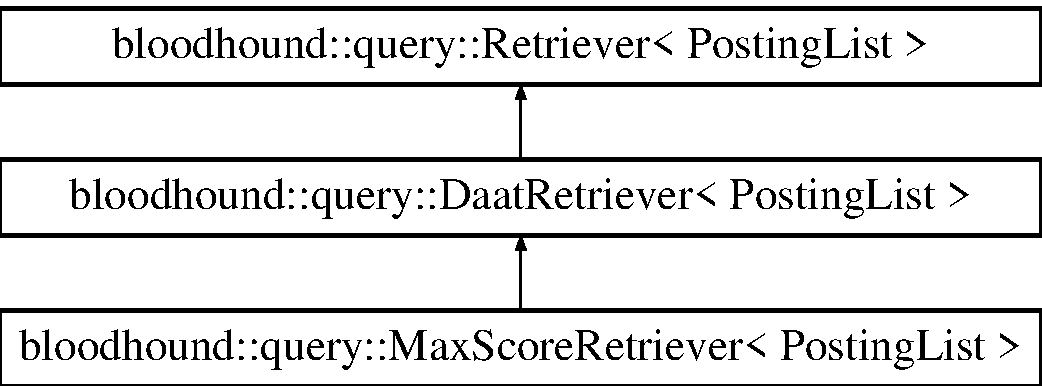
\includegraphics[height=3.000000cm]{classbloodhound_1_1query_1_1MaxScoreRetriever}
\end{center}
\end{figure}
\subsection*{Additional Inherited Members}


The documentation for this class was generated from the following file\+:\begin{DoxyCompactItemize}
\item 
include/\hyperlink{retrievers_8hpp}{retrievers.\+hpp}\end{DoxyCompactItemize}

\hypertarget{structbloodhound_1_1Offset}{}\section{bloodhound\+:\+:Offset Struct Reference}
\label{structbloodhound_1_1Offset}\index{bloodhound\+::\+Offset@{bloodhound\+::\+Offset}}


{\ttfamily \#include $<$index.\+hpp$>$}

Inheritance diagram for bloodhound\+:\+:Offset\+:\begin{figure}[H]
\begin{center}
\leavevmode
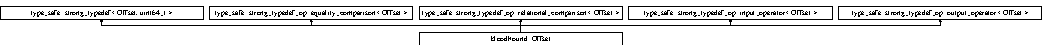
\includegraphics[height=0.598930cm]{structbloodhound_1_1Offset}
\end{center}
\end{figure}
\subsection*{Friends}
\begin{DoxyCompactItemize}
\item 
const char $\ast$ \mbox{\hyperlink{structbloodhound_1_1Offset_aaed86d39530be98502fa1560b323d07b}{operator+}} (const char $\ast$ptr, \mbox{\hyperlink{structbloodhound_1_1Offset}{Offset}} offset)
\item 
char $\ast$ \mbox{\hyperlink{structbloodhound_1_1Offset_aec6c323c060e7a7cae481422f1ecea7a}{operator+}} (char $\ast$ptr, \mbox{\hyperlink{structbloodhound_1_1Offset}{Offset}} offset)
\end{DoxyCompactItemize}


\subsection{Friends And Related Function Documentation}
\mbox{\Hypertarget{structbloodhound_1_1Offset_aaed86d39530be98502fa1560b323d07b}\label{structbloodhound_1_1Offset_aaed86d39530be98502fa1560b323d07b}} 
\index{bloodhound\+::\+Offset@{bloodhound\+::\+Offset}!operator+@{operator+}}
\index{operator+@{operator+}!bloodhound\+::\+Offset@{bloodhound\+::\+Offset}}
\subsubsection{\texorpdfstring{operator+}{operator+}\hspace{0.1cm}{\footnotesize\ttfamily [1/2]}}
{\footnotesize\ttfamily const char$\ast$ operator+ (\begin{DoxyParamCaption}\item[{const char $\ast$}]{ptr,  }\item[{\mbox{\hyperlink{structbloodhound_1_1Offset}{Offset}}}]{offset }\end{DoxyParamCaption})\hspace{0.3cm}{\ttfamily [friend]}}

\mbox{\Hypertarget{structbloodhound_1_1Offset_aec6c323c060e7a7cae481422f1ecea7a}\label{structbloodhound_1_1Offset_aec6c323c060e7a7cae481422f1ecea7a}} 
\index{bloodhound\+::\+Offset@{bloodhound\+::\+Offset}!operator+@{operator+}}
\index{operator+@{operator+}!bloodhound\+::\+Offset@{bloodhound\+::\+Offset}}
\subsubsection{\texorpdfstring{operator+}{operator+}\hspace{0.1cm}{\footnotesize\ttfamily [2/2]}}
{\footnotesize\ttfamily char$\ast$ operator+ (\begin{DoxyParamCaption}\item[{char $\ast$}]{ptr,  }\item[{\mbox{\hyperlink{structbloodhound_1_1Offset}{Offset}}}]{offset }\end{DoxyParamCaption})\hspace{0.3cm}{\ttfamily [friend]}}



The documentation for this struct was generated from the following file\+:\begin{DoxyCompactItemize}
\item 
include/\mbox{\hyperlink{index_8hpp}{index.\+hpp}}\end{DoxyCompactItemize}

\hypertarget{structbloodhound_1_1Posting}{}\section{bloodhound\+:\+:Posting Struct Reference}
\label{structbloodhound_1_1Posting}\index{bloodhound\+::\+Posting@{bloodhound\+::\+Posting}}


{\ttfamily \#include $<$index.\+hpp$>$}

\subsection*{Public Attributes}
\begin{DoxyCompactItemize}
\item 
\mbox{\hyperlink{structbloodhound_1_1Doc}{Doc}} \mbox{\hyperlink{structbloodhound_1_1Posting_ae39f120507b708385e754c693109e384}{doc}}
\item 
\mbox{\hyperlink{structbloodhound_1_1Score}{Score}} \mbox{\hyperlink{structbloodhound_1_1Posting_afcdc4c2d2486c04feee39077122e1622}{score}}
\end{DoxyCompactItemize}


\subsection{Member Data Documentation}
\mbox{\Hypertarget{structbloodhound_1_1Posting_ae39f120507b708385e754c693109e384}\label{structbloodhound_1_1Posting_ae39f120507b708385e754c693109e384}} 
\index{bloodhound\+::\+Posting@{bloodhound\+::\+Posting}!doc@{doc}}
\index{doc@{doc}!bloodhound\+::\+Posting@{bloodhound\+::\+Posting}}
\subsubsection{\texorpdfstring{doc}{doc}}
{\footnotesize\ttfamily \mbox{\hyperlink{structbloodhound_1_1Doc}{Doc}} bloodhound\+::\+Posting\+::doc}

\mbox{\Hypertarget{structbloodhound_1_1Posting_afcdc4c2d2486c04feee39077122e1622}\label{structbloodhound_1_1Posting_afcdc4c2d2486c04feee39077122e1622}} 
\index{bloodhound\+::\+Posting@{bloodhound\+::\+Posting}!score@{score}}
\index{score@{score}!bloodhound\+::\+Posting@{bloodhound\+::\+Posting}}
\subsubsection{\texorpdfstring{score}{score}}
{\footnotesize\ttfamily \mbox{\hyperlink{structbloodhound_1_1Score}{Score}} bloodhound\+::\+Posting\+::score}



The documentation for this struct was generated from the following file\+:\begin{DoxyCompactItemize}
\item 
include/\mbox{\hyperlink{index_8hpp}{index.\+hpp}}\end{DoxyCompactItemize}

\hypertarget{classbloodhound_1_1PostingList}{}\section{bloodhound\+:\+:Posting\+List Class Reference}
\label{classbloodhound_1_1PostingList}\index{bloodhound\+::\+Posting\+List@{bloodhound\+::\+Posting\+List}}


{\ttfamily \#include $<$index.\+hpp$>$}

\subsection*{Classes}
\begin{DoxyCompactItemize}
\item 
struct \mbox{\hyperlink{structbloodhound_1_1PostingList_1_1const__iterator}{const\+\_\+iterator}}
\item 
struct \mbox{\hyperlink{structbloodhound_1_1PostingList_1_1iterator}{iterator}}
\end{DoxyCompactItemize}
\subsection*{Public Member Functions}
\begin{DoxyCompactItemize}
\item 
\mbox{\hyperlink{classbloodhound_1_1PostingList_a725f1df76c8278f1d927fff3ed4c496e}{Posting\+List}} (\mbox{\hyperlink{structbloodhound_1_1Doc}{Doc}} $\ast$d, \mbox{\hyperlink{structbloodhound_1_1Score}{Score}} $\ast$s, uint32\+\_\+t l, \mbox{\hyperlink{structbloodhound_1_1Score}{Score}} ms)
\item 
std\+::size\+\_\+t \mbox{\hyperlink{classbloodhound_1_1PostingList_a7af6f4e9fc277dd7c1dc73c2922ceacd}{length}} () const
\item 
std\+::size\+\_\+t \mbox{\hyperlink{classbloodhound_1_1PostingList_a440e43337385c66edb4e1c0568c74544}{size}} () const
\item 
bool \mbox{\hyperlink{classbloodhound_1_1PostingList_a28ec60331aec6acaa9c281d4d412bf26}{empty}} () const
\item 
\mbox{\hyperlink{structbloodhound_1_1PostingList_1_1iterator}{iterator}} \mbox{\hyperlink{classbloodhound_1_1PostingList_abd082192a0339062d318de73c95f1ee5}{next\+\_\+ge}} (\mbox{\hyperlink{structbloodhound_1_1PostingList_1_1iterator}{iterator}} current, \mbox{\hyperlink{structbloodhound_1_1Doc}{Doc}} doc) const
\item 
\mbox{\hyperlink{structbloodhound_1_1PostingList_1_1iterator}{iterator}} \mbox{\hyperlink{classbloodhound_1_1PostingList_aae5c35208d6fb36f611f952ba57add0f}{next\+\_\+ge}} (\mbox{\hyperlink{structbloodhound_1_1PostingList_1_1iterator}{iterator}} current, \mbox{\hyperlink{structbloodhound_1_1PostingList_1_1iterator}{iterator}} \mbox{\hyperlink{classbloodhound_1_1PostingList_a2e1f899bd04ae64e1318494d358ade94}{end}}, \mbox{\hyperlink{structbloodhound_1_1Doc}{Doc}} doc) const
\item 
virtual \mbox{\hyperlink{structbloodhound_1_1PostingList_1_1iterator}{iterator}} \mbox{\hyperlink{classbloodhound_1_1PostingList_a274f57f133cd6763e0d8cc3e00fa1be3}{begin}} () const
\item 
virtual \mbox{\hyperlink{structbloodhound_1_1PostingList_1_1iterator}{iterator}} \mbox{\hyperlink{classbloodhound_1_1PostingList_a2e1f899bd04ae64e1318494d358ade94}{end}} () const
\item 
virtual \mbox{\hyperlink{structbloodhound_1_1PostingList_1_1const__iterator}{const\+\_\+iterator}} \mbox{\hyperlink{classbloodhound_1_1PostingList_a44980317210bfe6c9f7d59dbea1cbd4a}{cbegin}} () const
\item 
virtual \mbox{\hyperlink{structbloodhound_1_1PostingList_1_1const__iterator}{const\+\_\+iterator}} \mbox{\hyperlink{classbloodhound_1_1PostingList_a7eca0ae1f54ddc48757a4fb3c0b885ce}{cend}} () const
\item 
virtual gsl\+::span$<$ \mbox{\hyperlink{structbloodhound_1_1Doc}{Doc}} $>$\+::\mbox{\hyperlink{structbloodhound_1_1PostingList_1_1const__iterator}{const\+\_\+iterator}} \mbox{\hyperlink{classbloodhound_1_1PostingList_aac3dbe7fbf43ce93031e97b16bcfc888}{doc\+\_\+begin}} () const
\item 
virtual gsl\+::span$<$ \mbox{\hyperlink{structbloodhound_1_1Doc}{Doc}} $>$\+::\mbox{\hyperlink{structbloodhound_1_1PostingList_1_1const__iterator}{const\+\_\+iterator}} \mbox{\hyperlink{classbloodhound_1_1PostingList_aac468540b0a376d9b378a4333546245c}{doc\+\_\+end}} () const
\item 
virtual gsl\+::span$<$ \mbox{\hyperlink{structbloodhound_1_1Score}{Score}} $>$\+::\mbox{\hyperlink{structbloodhound_1_1PostingList_1_1const__iterator}{const\+\_\+iterator}} \mbox{\hyperlink{classbloodhound_1_1PostingList_aec5d5bb81622fb64d7b64416a8491456}{score\+\_\+begin}} () const
\item 
virtual gsl\+::span$<$ \mbox{\hyperlink{structbloodhound_1_1Score}{Score}} $>$\+::\mbox{\hyperlink{structbloodhound_1_1PostingList_1_1const__iterator}{const\+\_\+iterator}} \mbox{\hyperlink{classbloodhound_1_1PostingList_ae89abf9882f73f35a6e106c5a328ca6f}{score\+\_\+end}} () const
\item 
void \mbox{\hyperlink{classbloodhound_1_1PostingList_a3c9d6c5e88a7aae2642ff1d0f52160c0}{make\+\_\+et}} (double et\+\_\+threshold)
\item 
\mbox{\hyperlink{structbloodhound_1_1Doc}{Doc}} $\ast$ \mbox{\hyperlink{classbloodhound_1_1PostingList_acfca9e8ad1fd94461b56390fdd60779f}{docs\+\_\+ptr}} () const
\item 
\mbox{\hyperlink{structbloodhound_1_1Score}{Score}} $\ast$ \mbox{\hyperlink{classbloodhound_1_1PostingList_a79be9c874bb91e17ca308ae0528e9277}{scores\+\_\+ptr}} () const
\end{DoxyCompactItemize}
\subsection*{Public Attributes}
\begin{DoxyCompactItemize}
\item 
gsl\+::span$<$ \mbox{\hyperlink{structbloodhound_1_1Doc}{Doc}} $>$ \mbox{\hyperlink{classbloodhound_1_1PostingList_a11749c12634d86c73b7d9c150acaac03}{docs}}
\item 
gsl\+::span$<$ \mbox{\hyperlink{structbloodhound_1_1Score}{Score}} $>$ \mbox{\hyperlink{classbloodhound_1_1PostingList_a2c773bffa3d78d2e7a7e04d918b064da}{scores}}
\item 
\mbox{\hyperlink{structbloodhound_1_1Score}{Score}} \mbox{\hyperlink{classbloodhound_1_1PostingList_ab840a6f9ddf8de353cbdd09b3a184bfa}{max\+\_\+score}}
\item 
std\+::size\+\_\+t \mbox{\hyperlink{classbloodhound_1_1PostingList_a9aa9a9d1db46c6858fa952a36e1bf8fa}{idx}}
\item 
std\+::size\+\_\+t \mbox{\hyperlink{classbloodhound_1_1PostingList_a7c4d53dfa824951670d68ef57cd2068d}{end\+\_\+idx}}
\end{DoxyCompactItemize}


\subsection{Constructor \& Destructor Documentation}
\mbox{\Hypertarget{classbloodhound_1_1PostingList_a725f1df76c8278f1d927fff3ed4c496e}\label{classbloodhound_1_1PostingList_a725f1df76c8278f1d927fff3ed4c496e}} 
\index{bloodhound\+::\+Posting\+List@{bloodhound\+::\+Posting\+List}!Posting\+List@{Posting\+List}}
\index{Posting\+List@{Posting\+List}!bloodhound\+::\+Posting\+List@{bloodhound\+::\+Posting\+List}}
\subsubsection{\texorpdfstring{Posting\+List()}{PostingList()}}
{\footnotesize\ttfamily bloodhound\+::\+Posting\+List\+::\+Posting\+List (\begin{DoxyParamCaption}\item[{\mbox{\hyperlink{structbloodhound_1_1Doc}{Doc}} $\ast$}]{d,  }\item[{\mbox{\hyperlink{structbloodhound_1_1Score}{Score}} $\ast$}]{s,  }\item[{uint32\+\_\+t}]{l,  }\item[{\mbox{\hyperlink{structbloodhound_1_1Score}{Score}}}]{ms }\end{DoxyParamCaption})\hspace{0.3cm}{\ttfamily [inline]}}



\subsection{Member Function Documentation}
\mbox{\Hypertarget{classbloodhound_1_1PostingList_a274f57f133cd6763e0d8cc3e00fa1be3}\label{classbloodhound_1_1PostingList_a274f57f133cd6763e0d8cc3e00fa1be3}} 
\index{bloodhound\+::\+Posting\+List@{bloodhound\+::\+Posting\+List}!begin@{begin}}
\index{begin@{begin}!bloodhound\+::\+Posting\+List@{bloodhound\+::\+Posting\+List}}
\subsubsection{\texorpdfstring{begin()}{begin()}}
{\footnotesize\ttfamily virtual \mbox{\hyperlink{structbloodhound_1_1PostingList_1_1iterator}{iterator}} bloodhound\+::\+Posting\+List\+::begin (\begin{DoxyParamCaption}{ }\end{DoxyParamCaption}) const\hspace{0.3cm}{\ttfamily [inline]}, {\ttfamily [virtual]}}

\mbox{\Hypertarget{classbloodhound_1_1PostingList_a44980317210bfe6c9f7d59dbea1cbd4a}\label{classbloodhound_1_1PostingList_a44980317210bfe6c9f7d59dbea1cbd4a}} 
\index{bloodhound\+::\+Posting\+List@{bloodhound\+::\+Posting\+List}!cbegin@{cbegin}}
\index{cbegin@{cbegin}!bloodhound\+::\+Posting\+List@{bloodhound\+::\+Posting\+List}}
\subsubsection{\texorpdfstring{cbegin()}{cbegin()}}
{\footnotesize\ttfamily virtual \mbox{\hyperlink{structbloodhound_1_1PostingList_1_1const__iterator}{const\+\_\+iterator}} bloodhound\+::\+Posting\+List\+::cbegin (\begin{DoxyParamCaption}{ }\end{DoxyParamCaption}) const\hspace{0.3cm}{\ttfamily [inline]}, {\ttfamily [virtual]}}

\mbox{\Hypertarget{classbloodhound_1_1PostingList_a7eca0ae1f54ddc48757a4fb3c0b885ce}\label{classbloodhound_1_1PostingList_a7eca0ae1f54ddc48757a4fb3c0b885ce}} 
\index{bloodhound\+::\+Posting\+List@{bloodhound\+::\+Posting\+List}!cend@{cend}}
\index{cend@{cend}!bloodhound\+::\+Posting\+List@{bloodhound\+::\+Posting\+List}}
\subsubsection{\texorpdfstring{cend()}{cend()}}
{\footnotesize\ttfamily virtual \mbox{\hyperlink{structbloodhound_1_1PostingList_1_1const__iterator}{const\+\_\+iterator}} bloodhound\+::\+Posting\+List\+::cend (\begin{DoxyParamCaption}{ }\end{DoxyParamCaption}) const\hspace{0.3cm}{\ttfamily [inline]}, {\ttfamily [virtual]}}

\mbox{\Hypertarget{classbloodhound_1_1PostingList_aac3dbe7fbf43ce93031e97b16bcfc888}\label{classbloodhound_1_1PostingList_aac3dbe7fbf43ce93031e97b16bcfc888}} 
\index{bloodhound\+::\+Posting\+List@{bloodhound\+::\+Posting\+List}!doc\+\_\+begin@{doc\+\_\+begin}}
\index{doc\+\_\+begin@{doc\+\_\+begin}!bloodhound\+::\+Posting\+List@{bloodhound\+::\+Posting\+List}}
\subsubsection{\texorpdfstring{doc\+\_\+begin()}{doc\_begin()}}
{\footnotesize\ttfamily virtual gsl\+::span$<$\mbox{\hyperlink{structbloodhound_1_1Doc}{Doc}}$>$\+::\mbox{\hyperlink{structbloodhound_1_1PostingList_1_1const__iterator}{const\+\_\+iterator}} bloodhound\+::\+Posting\+List\+::doc\+\_\+begin (\begin{DoxyParamCaption}{ }\end{DoxyParamCaption}) const\hspace{0.3cm}{\ttfamily [inline]}, {\ttfamily [virtual]}}

\mbox{\Hypertarget{classbloodhound_1_1PostingList_aac468540b0a376d9b378a4333546245c}\label{classbloodhound_1_1PostingList_aac468540b0a376d9b378a4333546245c}} 
\index{bloodhound\+::\+Posting\+List@{bloodhound\+::\+Posting\+List}!doc\+\_\+end@{doc\+\_\+end}}
\index{doc\+\_\+end@{doc\+\_\+end}!bloodhound\+::\+Posting\+List@{bloodhound\+::\+Posting\+List}}
\subsubsection{\texorpdfstring{doc\+\_\+end()}{doc\_end()}}
{\footnotesize\ttfamily virtual gsl\+::span$<$\mbox{\hyperlink{structbloodhound_1_1Doc}{Doc}}$>$\+::\mbox{\hyperlink{structbloodhound_1_1PostingList_1_1const__iterator}{const\+\_\+iterator}} bloodhound\+::\+Posting\+List\+::doc\+\_\+end (\begin{DoxyParamCaption}{ }\end{DoxyParamCaption}) const\hspace{0.3cm}{\ttfamily [inline]}, {\ttfamily [virtual]}}

\mbox{\Hypertarget{classbloodhound_1_1PostingList_acfca9e8ad1fd94461b56390fdd60779f}\label{classbloodhound_1_1PostingList_acfca9e8ad1fd94461b56390fdd60779f}} 
\index{bloodhound\+::\+Posting\+List@{bloodhound\+::\+Posting\+List}!docs\+\_\+ptr@{docs\+\_\+ptr}}
\index{docs\+\_\+ptr@{docs\+\_\+ptr}!bloodhound\+::\+Posting\+List@{bloodhound\+::\+Posting\+List}}
\subsubsection{\texorpdfstring{docs\+\_\+ptr()}{docs\_ptr()}}
{\footnotesize\ttfamily \mbox{\hyperlink{structbloodhound_1_1Doc}{Doc}}$\ast$ bloodhound\+::\+Posting\+List\+::docs\+\_\+ptr (\begin{DoxyParamCaption}{ }\end{DoxyParamCaption}) const\hspace{0.3cm}{\ttfamily [inline]}}

\mbox{\Hypertarget{classbloodhound_1_1PostingList_a28ec60331aec6acaa9c281d4d412bf26}\label{classbloodhound_1_1PostingList_a28ec60331aec6acaa9c281d4d412bf26}} 
\index{bloodhound\+::\+Posting\+List@{bloodhound\+::\+Posting\+List}!empty@{empty}}
\index{empty@{empty}!bloodhound\+::\+Posting\+List@{bloodhound\+::\+Posting\+List}}
\subsubsection{\texorpdfstring{empty()}{empty()}}
{\footnotesize\ttfamily bool bloodhound\+::\+Posting\+List\+::empty (\begin{DoxyParamCaption}{ }\end{DoxyParamCaption}) const\hspace{0.3cm}{\ttfamily [inline]}}

\mbox{\Hypertarget{classbloodhound_1_1PostingList_a2e1f899bd04ae64e1318494d358ade94}\label{classbloodhound_1_1PostingList_a2e1f899bd04ae64e1318494d358ade94}} 
\index{bloodhound\+::\+Posting\+List@{bloodhound\+::\+Posting\+List}!end@{end}}
\index{end@{end}!bloodhound\+::\+Posting\+List@{bloodhound\+::\+Posting\+List}}
\subsubsection{\texorpdfstring{end()}{end()}}
{\footnotesize\ttfamily virtual \mbox{\hyperlink{structbloodhound_1_1PostingList_1_1iterator}{iterator}} bloodhound\+::\+Posting\+List\+::end (\begin{DoxyParamCaption}{ }\end{DoxyParamCaption}) const\hspace{0.3cm}{\ttfamily [inline]}, {\ttfamily [virtual]}}

\mbox{\Hypertarget{classbloodhound_1_1PostingList_a7af6f4e9fc277dd7c1dc73c2922ceacd}\label{classbloodhound_1_1PostingList_a7af6f4e9fc277dd7c1dc73c2922ceacd}} 
\index{bloodhound\+::\+Posting\+List@{bloodhound\+::\+Posting\+List}!length@{length}}
\index{length@{length}!bloodhound\+::\+Posting\+List@{bloodhound\+::\+Posting\+List}}
\subsubsection{\texorpdfstring{length()}{length()}}
{\footnotesize\ttfamily std\+::size\+\_\+t bloodhound\+::\+Posting\+List\+::length (\begin{DoxyParamCaption}{ }\end{DoxyParamCaption}) const\hspace{0.3cm}{\ttfamily [inline]}}

\mbox{\Hypertarget{classbloodhound_1_1PostingList_a3c9d6c5e88a7aae2642ff1d0f52160c0}\label{classbloodhound_1_1PostingList_a3c9d6c5e88a7aae2642ff1d0f52160c0}} 
\index{bloodhound\+::\+Posting\+List@{bloodhound\+::\+Posting\+List}!make\+\_\+et@{make\+\_\+et}}
\index{make\+\_\+et@{make\+\_\+et}!bloodhound\+::\+Posting\+List@{bloodhound\+::\+Posting\+List}}
\subsubsection{\texorpdfstring{make\+\_\+et()}{make\_et()}}
{\footnotesize\ttfamily void bloodhound\+::\+Posting\+List\+::make\+\_\+et (\begin{DoxyParamCaption}\item[{double}]{et\+\_\+threshold }\end{DoxyParamCaption})\hspace{0.3cm}{\ttfamily [inline]}}

\mbox{\Hypertarget{classbloodhound_1_1PostingList_abd082192a0339062d318de73c95f1ee5}\label{classbloodhound_1_1PostingList_abd082192a0339062d318de73c95f1ee5}} 
\index{bloodhound\+::\+Posting\+List@{bloodhound\+::\+Posting\+List}!next\+\_\+ge@{next\+\_\+ge}}
\index{next\+\_\+ge@{next\+\_\+ge}!bloodhound\+::\+Posting\+List@{bloodhound\+::\+Posting\+List}}
\subsubsection{\texorpdfstring{next\+\_\+ge()}{next\_ge()}\hspace{0.1cm}{\footnotesize\ttfamily [1/2]}}
{\footnotesize\ttfamily \mbox{\hyperlink{structbloodhound_1_1PostingList_1_1iterator}{iterator}} bloodhound\+::\+Posting\+List\+::next\+\_\+ge (\begin{DoxyParamCaption}\item[{\mbox{\hyperlink{structbloodhound_1_1PostingList_1_1iterator}{iterator}}}]{current,  }\item[{\mbox{\hyperlink{structbloodhound_1_1Doc}{Doc}}}]{doc }\end{DoxyParamCaption}) const\hspace{0.3cm}{\ttfamily [inline]}}

\mbox{\Hypertarget{classbloodhound_1_1PostingList_aae5c35208d6fb36f611f952ba57add0f}\label{classbloodhound_1_1PostingList_aae5c35208d6fb36f611f952ba57add0f}} 
\index{bloodhound\+::\+Posting\+List@{bloodhound\+::\+Posting\+List}!next\+\_\+ge@{next\+\_\+ge}}
\index{next\+\_\+ge@{next\+\_\+ge}!bloodhound\+::\+Posting\+List@{bloodhound\+::\+Posting\+List}}
\subsubsection{\texorpdfstring{next\+\_\+ge()}{next\_ge()}\hspace{0.1cm}{\footnotesize\ttfamily [2/2]}}
{\footnotesize\ttfamily \mbox{\hyperlink{structbloodhound_1_1PostingList_1_1iterator}{iterator}} bloodhound\+::\+Posting\+List\+::next\+\_\+ge (\begin{DoxyParamCaption}\item[{\mbox{\hyperlink{structbloodhound_1_1PostingList_1_1iterator}{iterator}}}]{current,  }\item[{\mbox{\hyperlink{structbloodhound_1_1PostingList_1_1iterator}{iterator}}}]{end,  }\item[{\mbox{\hyperlink{structbloodhound_1_1Doc}{Doc}}}]{doc }\end{DoxyParamCaption}) const\hspace{0.3cm}{\ttfamily [inline]}}

\mbox{\Hypertarget{classbloodhound_1_1PostingList_aec5d5bb81622fb64d7b64416a8491456}\label{classbloodhound_1_1PostingList_aec5d5bb81622fb64d7b64416a8491456}} 
\index{bloodhound\+::\+Posting\+List@{bloodhound\+::\+Posting\+List}!score\+\_\+begin@{score\+\_\+begin}}
\index{score\+\_\+begin@{score\+\_\+begin}!bloodhound\+::\+Posting\+List@{bloodhound\+::\+Posting\+List}}
\subsubsection{\texorpdfstring{score\+\_\+begin()}{score\_begin()}}
{\footnotesize\ttfamily virtual gsl\+::span$<$\mbox{\hyperlink{structbloodhound_1_1Score}{Score}}$>$\+::\mbox{\hyperlink{structbloodhound_1_1PostingList_1_1const__iterator}{const\+\_\+iterator}} bloodhound\+::\+Posting\+List\+::score\+\_\+begin (\begin{DoxyParamCaption}{ }\end{DoxyParamCaption}) const\hspace{0.3cm}{\ttfamily [inline]}, {\ttfamily [virtual]}}

\mbox{\Hypertarget{classbloodhound_1_1PostingList_ae89abf9882f73f35a6e106c5a328ca6f}\label{classbloodhound_1_1PostingList_ae89abf9882f73f35a6e106c5a328ca6f}} 
\index{bloodhound\+::\+Posting\+List@{bloodhound\+::\+Posting\+List}!score\+\_\+end@{score\+\_\+end}}
\index{score\+\_\+end@{score\+\_\+end}!bloodhound\+::\+Posting\+List@{bloodhound\+::\+Posting\+List}}
\subsubsection{\texorpdfstring{score\+\_\+end()}{score\_end()}}
{\footnotesize\ttfamily virtual gsl\+::span$<$\mbox{\hyperlink{structbloodhound_1_1Score}{Score}}$>$\+::\mbox{\hyperlink{structbloodhound_1_1PostingList_1_1const__iterator}{const\+\_\+iterator}} bloodhound\+::\+Posting\+List\+::score\+\_\+end (\begin{DoxyParamCaption}{ }\end{DoxyParamCaption}) const\hspace{0.3cm}{\ttfamily [inline]}, {\ttfamily [virtual]}}

\mbox{\Hypertarget{classbloodhound_1_1PostingList_a79be9c874bb91e17ca308ae0528e9277}\label{classbloodhound_1_1PostingList_a79be9c874bb91e17ca308ae0528e9277}} 
\index{bloodhound\+::\+Posting\+List@{bloodhound\+::\+Posting\+List}!scores\+\_\+ptr@{scores\+\_\+ptr}}
\index{scores\+\_\+ptr@{scores\+\_\+ptr}!bloodhound\+::\+Posting\+List@{bloodhound\+::\+Posting\+List}}
\subsubsection{\texorpdfstring{scores\+\_\+ptr()}{scores\_ptr()}}
{\footnotesize\ttfamily \mbox{\hyperlink{structbloodhound_1_1Score}{Score}}$\ast$ bloodhound\+::\+Posting\+List\+::scores\+\_\+ptr (\begin{DoxyParamCaption}{ }\end{DoxyParamCaption}) const\hspace{0.3cm}{\ttfamily [inline]}}

\mbox{\Hypertarget{classbloodhound_1_1PostingList_a440e43337385c66edb4e1c0568c74544}\label{classbloodhound_1_1PostingList_a440e43337385c66edb4e1c0568c74544}} 
\index{bloodhound\+::\+Posting\+List@{bloodhound\+::\+Posting\+List}!size@{size}}
\index{size@{size}!bloodhound\+::\+Posting\+List@{bloodhound\+::\+Posting\+List}}
\subsubsection{\texorpdfstring{size()}{size()}}
{\footnotesize\ttfamily std\+::size\+\_\+t bloodhound\+::\+Posting\+List\+::size (\begin{DoxyParamCaption}{ }\end{DoxyParamCaption}) const\hspace{0.3cm}{\ttfamily [inline]}}



\subsection{Member Data Documentation}
\mbox{\Hypertarget{classbloodhound_1_1PostingList_a11749c12634d86c73b7d9c150acaac03}\label{classbloodhound_1_1PostingList_a11749c12634d86c73b7d9c150acaac03}} 
\index{bloodhound\+::\+Posting\+List@{bloodhound\+::\+Posting\+List}!docs@{docs}}
\index{docs@{docs}!bloodhound\+::\+Posting\+List@{bloodhound\+::\+Posting\+List}}
\subsubsection{\texorpdfstring{docs}{docs}}
{\footnotesize\ttfamily gsl\+::span$<$\mbox{\hyperlink{structbloodhound_1_1Doc}{Doc}}$>$ bloodhound\+::\+Posting\+List\+::docs}

\mbox{\Hypertarget{classbloodhound_1_1PostingList_a7c4d53dfa824951670d68ef57cd2068d}\label{classbloodhound_1_1PostingList_a7c4d53dfa824951670d68ef57cd2068d}} 
\index{bloodhound\+::\+Posting\+List@{bloodhound\+::\+Posting\+List}!end\+\_\+idx@{end\+\_\+idx}}
\index{end\+\_\+idx@{end\+\_\+idx}!bloodhound\+::\+Posting\+List@{bloodhound\+::\+Posting\+List}}
\subsubsection{\texorpdfstring{end\+\_\+idx}{end\_idx}}
{\footnotesize\ttfamily std\+::size\+\_\+t bloodhound\+::\+Posting\+List\+::end\+\_\+idx}

\mbox{\Hypertarget{classbloodhound_1_1PostingList_a9aa9a9d1db46c6858fa952a36e1bf8fa}\label{classbloodhound_1_1PostingList_a9aa9a9d1db46c6858fa952a36e1bf8fa}} 
\index{bloodhound\+::\+Posting\+List@{bloodhound\+::\+Posting\+List}!idx@{idx}}
\index{idx@{idx}!bloodhound\+::\+Posting\+List@{bloodhound\+::\+Posting\+List}}
\subsubsection{\texorpdfstring{idx}{idx}}
{\footnotesize\ttfamily std\+::size\+\_\+t bloodhound\+::\+Posting\+List\+::idx}

\mbox{\Hypertarget{classbloodhound_1_1PostingList_ab840a6f9ddf8de353cbdd09b3a184bfa}\label{classbloodhound_1_1PostingList_ab840a6f9ddf8de353cbdd09b3a184bfa}} 
\index{bloodhound\+::\+Posting\+List@{bloodhound\+::\+Posting\+List}!max\+\_\+score@{max\+\_\+score}}
\index{max\+\_\+score@{max\+\_\+score}!bloodhound\+::\+Posting\+List@{bloodhound\+::\+Posting\+List}}
\subsubsection{\texorpdfstring{max\+\_\+score}{max\_score}}
{\footnotesize\ttfamily \mbox{\hyperlink{structbloodhound_1_1Score}{Score}} bloodhound\+::\+Posting\+List\+::max\+\_\+score}

\mbox{\Hypertarget{classbloodhound_1_1PostingList_a2c773bffa3d78d2e7a7e04d918b064da}\label{classbloodhound_1_1PostingList_a2c773bffa3d78d2e7a7e04d918b064da}} 
\index{bloodhound\+::\+Posting\+List@{bloodhound\+::\+Posting\+List}!scores@{scores}}
\index{scores@{scores}!bloodhound\+::\+Posting\+List@{bloodhound\+::\+Posting\+List}}
\subsubsection{\texorpdfstring{scores}{scores}}
{\footnotesize\ttfamily gsl\+::span$<$\mbox{\hyperlink{structbloodhound_1_1Score}{Score}}$>$ bloodhound\+::\+Posting\+List\+::scores}



The documentation for this class was generated from the following file\+:\begin{DoxyCompactItemize}
\item 
include/\mbox{\hyperlink{index_8hpp}{index.\+hpp}}\end{DoxyCompactItemize}

\hypertarget{structbloodhound_1_1index_1_1PostingListHeader}{}\section{bloodhound\+:\+:index\+:\+:Posting\+List\+Header Struct Reference}
\label{structbloodhound_1_1index_1_1PostingListHeader}\index{bloodhound\+::index\+::\+Posting\+List\+Header@{bloodhound\+::index\+::\+Posting\+List\+Header}}


{\ttfamily \#include $<$index.\+hpp$>$}

\subsection*{Public Member Functions}
\begin{DoxyCompactItemize}
\item 
\mbox{\hyperlink{structbloodhound_1_1index_1_1PostingListHeader_a839dc96a649a6a5b381b4e9b93b6e59e}{Posting\+List\+Header}} ()
\item 
\mbox{\hyperlink{structbloodhound_1_1index_1_1PostingListHeader_a9aec6f6c7099b8ea249dc8af709c2125}{Posting\+List\+Header}} (uint32\+\_\+t m, uint32\+\_\+t d, uint32\+\_\+t pc, uint32\+\_\+t pyo, uint32\+\_\+t poo, uint32\+\_\+t so)
\item 
bool \mbox{\hyperlink{structbloodhound_1_1index_1_1PostingListHeader_a4202dde165e19c7dceec520a19d753e9}{checkmask}} (int b) const
\item 
void \mbox{\hyperlink{structbloodhound_1_1index_1_1PostingListHeader_ab9bb3cd3201527041e86a7fec0bd385d}{setmask}} (int b)
\item 
bool \mbox{\hyperlink{structbloodhound_1_1index_1_1PostingListHeader_acf8fd2592a71083d37bb7bb58fc8c544}{is\+\_\+short}} () const
\end{DoxyCompactItemize}
\subsection*{Public Attributes}
\begin{DoxyCompactItemize}
\item 
uint32\+\_\+t \mbox{\hyperlink{structbloodhound_1_1index_1_1PostingListHeader_a18fbb5f0675f6e59844b599950809bb0}{mask}}
\item 
uint32\+\_\+t \mbox{\hyperlink{structbloodhound_1_1index_1_1PostingListHeader_ac22a6d1974badac6cbedfb69f9c9bf5c}{doc\+\_\+count}}
\item 
uint32\+\_\+t \mbox{\hyperlink{structbloodhound_1_1index_1_1PostingListHeader_a88360105ba2e46000621f5bb74b4269c}{position\+\_\+count}}
\item 
uint32\+\_\+t \mbox{\hyperlink{structbloodhound_1_1index_1_1PostingListHeader_ab4ff4ee2a0aa56e03d315f6e60adf345}{payload\+\_\+offset}}
\item 
uint32\+\_\+t \mbox{\hyperlink{structbloodhound_1_1index_1_1PostingListHeader_a656267fe79315c04f431f99c1c826fec}{position\+\_\+offset}}
\item 
uint32\+\_\+t \mbox{\hyperlink{structbloodhound_1_1index_1_1PostingListHeader_a0c073440a09f22e0e277d3935d6b9158}{section\+\_\+offset}}
\end{DoxyCompactItemize}


\subsection{Constructor \& Destructor Documentation}
\mbox{\Hypertarget{structbloodhound_1_1index_1_1PostingListHeader_a839dc96a649a6a5b381b4e9b93b6e59e}\label{structbloodhound_1_1index_1_1PostingListHeader_a839dc96a649a6a5b381b4e9b93b6e59e}} 
\index{bloodhound\+::index\+::\+Posting\+List\+Header@{bloodhound\+::index\+::\+Posting\+List\+Header}!Posting\+List\+Header@{Posting\+List\+Header}}
\index{Posting\+List\+Header@{Posting\+List\+Header}!bloodhound\+::index\+::\+Posting\+List\+Header@{bloodhound\+::index\+::\+Posting\+List\+Header}}
\subsubsection{\texorpdfstring{Posting\+List\+Header()}{PostingListHeader()}\hspace{0.1cm}{\footnotesize\ttfamily [1/2]}}
{\footnotesize\ttfamily bloodhound\+::index\+::\+Posting\+List\+Header\+::\+Posting\+List\+Header (\begin{DoxyParamCaption}{ }\end{DoxyParamCaption})\hspace{0.3cm}{\ttfamily [inline]}}

\mbox{\Hypertarget{structbloodhound_1_1index_1_1PostingListHeader_a9aec6f6c7099b8ea249dc8af709c2125}\label{structbloodhound_1_1index_1_1PostingListHeader_a9aec6f6c7099b8ea249dc8af709c2125}} 
\index{bloodhound\+::index\+::\+Posting\+List\+Header@{bloodhound\+::index\+::\+Posting\+List\+Header}!Posting\+List\+Header@{Posting\+List\+Header}}
\index{Posting\+List\+Header@{Posting\+List\+Header}!bloodhound\+::index\+::\+Posting\+List\+Header@{bloodhound\+::index\+::\+Posting\+List\+Header}}
\subsubsection{\texorpdfstring{Posting\+List\+Header()}{PostingListHeader()}\hspace{0.1cm}{\footnotesize\ttfamily [2/2]}}
{\footnotesize\ttfamily bloodhound\+::index\+::\+Posting\+List\+Header\+::\+Posting\+List\+Header (\begin{DoxyParamCaption}\item[{uint32\+\_\+t}]{m,  }\item[{uint32\+\_\+t}]{d,  }\item[{uint32\+\_\+t}]{pc,  }\item[{uint32\+\_\+t}]{pyo,  }\item[{uint32\+\_\+t}]{poo,  }\item[{uint32\+\_\+t}]{so }\end{DoxyParamCaption})\hspace{0.3cm}{\ttfamily [inline]}}



\subsection{Member Function Documentation}
\mbox{\Hypertarget{structbloodhound_1_1index_1_1PostingListHeader_a4202dde165e19c7dceec520a19d753e9}\label{structbloodhound_1_1index_1_1PostingListHeader_a4202dde165e19c7dceec520a19d753e9}} 
\index{bloodhound\+::index\+::\+Posting\+List\+Header@{bloodhound\+::index\+::\+Posting\+List\+Header}!checkmask@{checkmask}}
\index{checkmask@{checkmask}!bloodhound\+::index\+::\+Posting\+List\+Header@{bloodhound\+::index\+::\+Posting\+List\+Header}}
\subsubsection{\texorpdfstring{checkmask()}{checkmask()}}
{\footnotesize\ttfamily bool bloodhound\+::index\+::\+Posting\+List\+Header\+::checkmask (\begin{DoxyParamCaption}\item[{int}]{b }\end{DoxyParamCaption}) const\hspace{0.3cm}{\ttfamily [inline]}}

\mbox{\Hypertarget{structbloodhound_1_1index_1_1PostingListHeader_acf8fd2592a71083d37bb7bb58fc8c544}\label{structbloodhound_1_1index_1_1PostingListHeader_acf8fd2592a71083d37bb7bb58fc8c544}} 
\index{bloodhound\+::index\+::\+Posting\+List\+Header@{bloodhound\+::index\+::\+Posting\+List\+Header}!is\+\_\+short@{is\+\_\+short}}
\index{is\+\_\+short@{is\+\_\+short}!bloodhound\+::index\+::\+Posting\+List\+Header@{bloodhound\+::index\+::\+Posting\+List\+Header}}
\subsubsection{\texorpdfstring{is\+\_\+short()}{is\_short()}}
{\footnotesize\ttfamily bool bloodhound\+::index\+::\+Posting\+List\+Header\+::is\+\_\+short (\begin{DoxyParamCaption}{ }\end{DoxyParamCaption}) const\hspace{0.3cm}{\ttfamily [inline]}}

\mbox{\Hypertarget{structbloodhound_1_1index_1_1PostingListHeader_ab9bb3cd3201527041e86a7fec0bd385d}\label{structbloodhound_1_1index_1_1PostingListHeader_ab9bb3cd3201527041e86a7fec0bd385d}} 
\index{bloodhound\+::index\+::\+Posting\+List\+Header@{bloodhound\+::index\+::\+Posting\+List\+Header}!setmask@{setmask}}
\index{setmask@{setmask}!bloodhound\+::index\+::\+Posting\+List\+Header@{bloodhound\+::index\+::\+Posting\+List\+Header}}
\subsubsection{\texorpdfstring{setmask()}{setmask()}}
{\footnotesize\ttfamily void bloodhound\+::index\+::\+Posting\+List\+Header\+::setmask (\begin{DoxyParamCaption}\item[{int}]{b }\end{DoxyParamCaption})\hspace{0.3cm}{\ttfamily [inline]}}



\subsection{Member Data Documentation}
\mbox{\Hypertarget{structbloodhound_1_1index_1_1PostingListHeader_ac22a6d1974badac6cbedfb69f9c9bf5c}\label{structbloodhound_1_1index_1_1PostingListHeader_ac22a6d1974badac6cbedfb69f9c9bf5c}} 
\index{bloodhound\+::index\+::\+Posting\+List\+Header@{bloodhound\+::index\+::\+Posting\+List\+Header}!doc\+\_\+count@{doc\+\_\+count}}
\index{doc\+\_\+count@{doc\+\_\+count}!bloodhound\+::index\+::\+Posting\+List\+Header@{bloodhound\+::index\+::\+Posting\+List\+Header}}
\subsubsection{\texorpdfstring{doc\+\_\+count}{doc\_count}}
{\footnotesize\ttfamily uint32\+\_\+t bloodhound\+::index\+::\+Posting\+List\+Header\+::doc\+\_\+count}

\mbox{\Hypertarget{structbloodhound_1_1index_1_1PostingListHeader_a18fbb5f0675f6e59844b599950809bb0}\label{structbloodhound_1_1index_1_1PostingListHeader_a18fbb5f0675f6e59844b599950809bb0}} 
\index{bloodhound\+::index\+::\+Posting\+List\+Header@{bloodhound\+::index\+::\+Posting\+List\+Header}!mask@{mask}}
\index{mask@{mask}!bloodhound\+::index\+::\+Posting\+List\+Header@{bloodhound\+::index\+::\+Posting\+List\+Header}}
\subsubsection{\texorpdfstring{mask}{mask}}
{\footnotesize\ttfamily uint32\+\_\+t bloodhound\+::index\+::\+Posting\+List\+Header\+::mask}

\mbox{\Hypertarget{structbloodhound_1_1index_1_1PostingListHeader_ab4ff4ee2a0aa56e03d315f6e60adf345}\label{structbloodhound_1_1index_1_1PostingListHeader_ab4ff4ee2a0aa56e03d315f6e60adf345}} 
\index{bloodhound\+::index\+::\+Posting\+List\+Header@{bloodhound\+::index\+::\+Posting\+List\+Header}!payload\+\_\+offset@{payload\+\_\+offset}}
\index{payload\+\_\+offset@{payload\+\_\+offset}!bloodhound\+::index\+::\+Posting\+List\+Header@{bloodhound\+::index\+::\+Posting\+List\+Header}}
\subsubsection{\texorpdfstring{payload\+\_\+offset}{payload\_offset}}
{\footnotesize\ttfamily uint32\+\_\+t bloodhound\+::index\+::\+Posting\+List\+Header\+::payload\+\_\+offset}

\mbox{\Hypertarget{structbloodhound_1_1index_1_1PostingListHeader_a88360105ba2e46000621f5bb74b4269c}\label{structbloodhound_1_1index_1_1PostingListHeader_a88360105ba2e46000621f5bb74b4269c}} 
\index{bloodhound\+::index\+::\+Posting\+List\+Header@{bloodhound\+::index\+::\+Posting\+List\+Header}!position\+\_\+count@{position\+\_\+count}}
\index{position\+\_\+count@{position\+\_\+count}!bloodhound\+::index\+::\+Posting\+List\+Header@{bloodhound\+::index\+::\+Posting\+List\+Header}}
\subsubsection{\texorpdfstring{position\+\_\+count}{position\_count}}
{\footnotesize\ttfamily uint32\+\_\+t bloodhound\+::index\+::\+Posting\+List\+Header\+::position\+\_\+count}

\mbox{\Hypertarget{structbloodhound_1_1index_1_1PostingListHeader_a656267fe79315c04f431f99c1c826fec}\label{structbloodhound_1_1index_1_1PostingListHeader_a656267fe79315c04f431f99c1c826fec}} 
\index{bloodhound\+::index\+::\+Posting\+List\+Header@{bloodhound\+::index\+::\+Posting\+List\+Header}!position\+\_\+offset@{position\+\_\+offset}}
\index{position\+\_\+offset@{position\+\_\+offset}!bloodhound\+::index\+::\+Posting\+List\+Header@{bloodhound\+::index\+::\+Posting\+List\+Header}}
\subsubsection{\texorpdfstring{position\+\_\+offset}{position\_offset}}
{\footnotesize\ttfamily uint32\+\_\+t bloodhound\+::index\+::\+Posting\+List\+Header\+::position\+\_\+offset}

\mbox{\Hypertarget{structbloodhound_1_1index_1_1PostingListHeader_a0c073440a09f22e0e277d3935d6b9158}\label{structbloodhound_1_1index_1_1PostingListHeader_a0c073440a09f22e0e277d3935d6b9158}} 
\index{bloodhound\+::index\+::\+Posting\+List\+Header@{bloodhound\+::index\+::\+Posting\+List\+Header}!section\+\_\+offset@{section\+\_\+offset}}
\index{section\+\_\+offset@{section\+\_\+offset}!bloodhound\+::index\+::\+Posting\+List\+Header@{bloodhound\+::index\+::\+Posting\+List\+Header}}
\subsubsection{\texorpdfstring{section\+\_\+offset}{section\_offset}}
{\footnotesize\ttfamily uint32\+\_\+t bloodhound\+::index\+::\+Posting\+List\+Header\+::section\+\_\+offset}



The documentation for this struct was generated from the following file\+:\begin{DoxyCompactItemize}
\item 
include/\mbox{\hyperlink{index_8hpp}{index.\+hpp}}\end{DoxyCompactItemize}

\hypertarget{classbloodhound_1_1query_1_1RawTaatRetriever}{}\section{bloodhound\+:\+:query\+:\+:Raw\+Taat\+Retriever$<$ Posting\+List $>$ Class Template Reference}
\label{classbloodhound_1_1query_1_1RawTaatRetriever}\index{bloodhound\+::query\+::\+Raw\+Taat\+Retriever$<$ Posting\+List $>$@{bloodhound\+::query\+::\+Raw\+Taat\+Retriever$<$ Posting\+List $>$}}


{\ttfamily \#include $<$retrievers.\+hpp$>$}

Inheritance diagram for bloodhound\+:\+:query\+:\+:Raw\+Taat\+Retriever$<$ Posting\+List $>$\+:\begin{figure}[H]
\begin{center}
\leavevmode
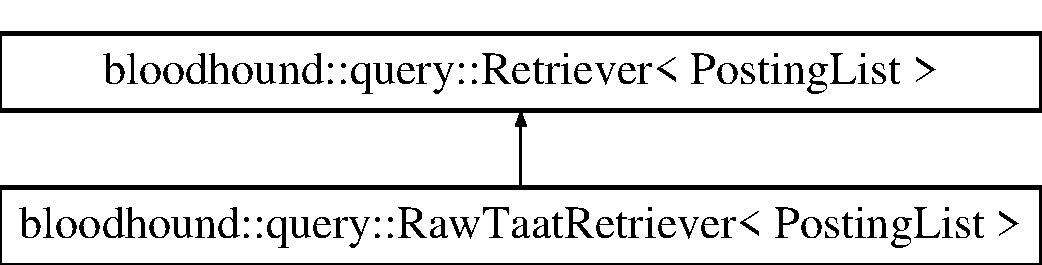
\includegraphics[height=2.000000cm]{classbloodhound_1_1query_1_1RawTaatRetriever}
\end{center}
\end{figure}
\subsection*{Public Member Functions}
\begin{DoxyCompactItemize}
\item 
\hyperlink{classbloodhound_1_1query_1_1RawTaatRetriever_a859b1cd2092da229964e2795c4445d72}{Raw\+Taat\+Retriever} (std\+::size\+\_\+t collection\+\_\+size)
\item 
void \hyperlink{classbloodhound_1_1query_1_1RawTaatRetriever_a70007a6dd5213e9c28266e38b424ba20}{traverse} (const std\+::vector$<$ \hyperlink{classbloodhound_1_1PostingList}{Posting\+List} $>$ \&lists\+\_\+for\+\_\+terms, const std\+::vector$<$ \hyperlink{structbloodhound_1_1Score}{Score} $>$ \&term\+\_\+weights)
\begin{DoxyCompactList}\small\item\em Traverses the postings and accumulates the scores. \end{DoxyCompactList}\item 
virtual std\+::vector$<$ \hyperlink{structbloodhound_1_1query_1_1Result}{Result} $>$ \hyperlink{classbloodhound_1_1query_1_1RawTaatRetriever_aafaaf842fdaef297a255e28766af2c0d}{retrieve} (const std\+::vector$<$ \hyperlink{classbloodhound_1_1PostingList}{Posting\+List} $>$ \&lists\+\_\+for\+\_\+terms, const std\+::vector$<$ \hyperlink{structbloodhound_1_1Score}{Score} $>$ \&term\+\_\+weights, std\+::size\+\_\+t k)
\begin{DoxyCompactList}\small\item\em Retrieves top-\/k results for the given posting lists and term weights. \end{DoxyCompactList}\end{DoxyCompactItemize}


\subsection{Constructor \& Destructor Documentation}
\mbox{\Hypertarget{classbloodhound_1_1query_1_1RawTaatRetriever_a859b1cd2092da229964e2795c4445d72}\label{classbloodhound_1_1query_1_1RawTaatRetriever_a859b1cd2092da229964e2795c4445d72}} 
\index{bloodhound\+::query\+::\+Raw\+Taat\+Retriever@{bloodhound\+::query\+::\+Raw\+Taat\+Retriever}!Raw\+Taat\+Retriever@{Raw\+Taat\+Retriever}}
\index{Raw\+Taat\+Retriever@{Raw\+Taat\+Retriever}!bloodhound\+::query\+::\+Raw\+Taat\+Retriever@{bloodhound\+::query\+::\+Raw\+Taat\+Retriever}}
\subsubsection{\texorpdfstring{Raw\+Taat\+Retriever()}{RawTaatRetriever()}}
{\footnotesize\ttfamily template$<$typename Posting\+List $>$ \\
\hyperlink{classbloodhound_1_1query_1_1RawTaatRetriever}{bloodhound\+::query\+::\+Raw\+Taat\+Retriever}$<$ \hyperlink{classbloodhound_1_1PostingList}{Posting\+List} $>$\+::\hyperlink{classbloodhound_1_1query_1_1RawTaatRetriever}{Raw\+Taat\+Retriever} (\begin{DoxyParamCaption}\item[{std\+::size\+\_\+t}]{collection\+\_\+size }\end{DoxyParamCaption})\hspace{0.3cm}{\ttfamily [inline]}}



\subsection{Member Function Documentation}
\mbox{\Hypertarget{classbloodhound_1_1query_1_1RawTaatRetriever_aafaaf842fdaef297a255e28766af2c0d}\label{classbloodhound_1_1query_1_1RawTaatRetriever_aafaaf842fdaef297a255e28766af2c0d}} 
\index{bloodhound\+::query\+::\+Raw\+Taat\+Retriever@{bloodhound\+::query\+::\+Raw\+Taat\+Retriever}!retrieve@{retrieve}}
\index{retrieve@{retrieve}!bloodhound\+::query\+::\+Raw\+Taat\+Retriever@{bloodhound\+::query\+::\+Raw\+Taat\+Retriever}}
\subsubsection{\texorpdfstring{retrieve()}{retrieve()}}
{\footnotesize\ttfamily template$<$typename Posting\+List $>$ \\
virtual std\+::vector$<$\hyperlink{structbloodhound_1_1query_1_1Result}{Result}$>$ \hyperlink{classbloodhound_1_1query_1_1RawTaatRetriever}{bloodhound\+::query\+::\+Raw\+Taat\+Retriever}$<$ \hyperlink{classbloodhound_1_1PostingList}{Posting\+List} $>$\+::retrieve (\begin{DoxyParamCaption}\item[{const std\+::vector$<$ \hyperlink{classbloodhound_1_1PostingList}{Posting\+List} $>$ \&}]{term\+\_\+postings,  }\item[{const std\+::vector$<$ \hyperlink{structbloodhound_1_1Score}{Score} $>$ \&}]{term\+\_\+weights,  }\item[{std\+::size\+\_\+t}]{k }\end{DoxyParamCaption})\hspace{0.3cm}{\ttfamily [inline]}, {\ttfamily [virtual]}}



Retrieves top-\/k results for the given posting lists and term weights. 



Implements \hyperlink{classbloodhound_1_1query_1_1Retriever_ae3c6a4628c5580e620c213b3dcd47c2b}{bloodhound\+::query\+::\+Retriever$<$ Posting\+List $>$}.

\mbox{\Hypertarget{classbloodhound_1_1query_1_1RawTaatRetriever_a70007a6dd5213e9c28266e38b424ba20}\label{classbloodhound_1_1query_1_1RawTaatRetriever_a70007a6dd5213e9c28266e38b424ba20}} 
\index{bloodhound\+::query\+::\+Raw\+Taat\+Retriever@{bloodhound\+::query\+::\+Raw\+Taat\+Retriever}!traverse@{traverse}}
\index{traverse@{traverse}!bloodhound\+::query\+::\+Raw\+Taat\+Retriever@{bloodhound\+::query\+::\+Raw\+Taat\+Retriever}}
\subsubsection{\texorpdfstring{traverse()}{traverse()}}
{\footnotesize\ttfamily template$<$typename Posting\+List $>$ \\
void \hyperlink{classbloodhound_1_1query_1_1RawTaatRetriever}{bloodhound\+::query\+::\+Raw\+Taat\+Retriever}$<$ \hyperlink{classbloodhound_1_1PostingList}{Posting\+List} $>$\+::traverse (\begin{DoxyParamCaption}\item[{const std\+::vector$<$ \hyperlink{classbloodhound_1_1PostingList}{Posting\+List} $>$ \&}]{lists\+\_\+for\+\_\+terms,  }\item[{const std\+::vector$<$ \hyperlink{structbloodhound_1_1Score}{Score} $>$ \&}]{term\+\_\+weights }\end{DoxyParamCaption})\hspace{0.3cm}{\ttfamily [inline]}}



Traverses the postings and accumulates the scores. 



The documentation for this class was generated from the following file\+:\begin{DoxyCompactItemize}
\item 
include/\hyperlink{retrievers_8hpp}{retrievers.\+hpp}\end{DoxyCompactItemize}

\hypertarget{structbloodhound_1_1RelativeOffset}{}\section{bloodhound\+:\+:Relative\+Offset Struct Reference}
\label{structbloodhound_1_1RelativeOffset}\index{bloodhound\+::\+Relative\+Offset@{bloodhound\+::\+Relative\+Offset}}


{\ttfamily \#include $<$index.\+hpp$>$}

Inheritance diagram for bloodhound\+:\+:Relative\+Offset\+:\begin{figure}[H]
\begin{center}
\leavevmode
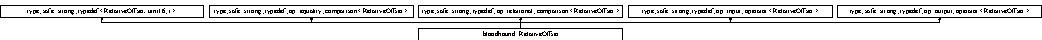
\includegraphics[height=0.534606cm]{structbloodhound_1_1RelativeOffset}
\end{center}
\end{figure}
\subsection*{Friends}
\begin{DoxyCompactItemize}
\item 
const char $\ast$ \hyperlink{structbloodhound_1_1RelativeOffset_a878bac48143c1d3b2597273daca07f25}{operator+} (const char $\ast$ptr, \hyperlink{structbloodhound_1_1RelativeOffset}{Relative\+Offset} offset)
\item 
char $\ast$ \hyperlink{structbloodhound_1_1RelativeOffset_aef76589aeb04376cde5936475652ceda}{operator+} (char $\ast$ptr, \hyperlink{structbloodhound_1_1RelativeOffset}{Relative\+Offset} offset)
\end{DoxyCompactItemize}


\subsection{Friends And Related Function Documentation}
\mbox{\Hypertarget{structbloodhound_1_1RelativeOffset_a878bac48143c1d3b2597273daca07f25}\label{structbloodhound_1_1RelativeOffset_a878bac48143c1d3b2597273daca07f25}} 
\index{bloodhound\+::\+Relative\+Offset@{bloodhound\+::\+Relative\+Offset}!operator+@{operator+}}
\index{operator+@{operator+}!bloodhound\+::\+Relative\+Offset@{bloodhound\+::\+Relative\+Offset}}
\subsubsection{\texorpdfstring{operator+}{operator+}\hspace{0.1cm}{\footnotesize\ttfamily [1/2]}}
{\footnotesize\ttfamily const char$\ast$ operator+ (\begin{DoxyParamCaption}\item[{const char $\ast$}]{ptr,  }\item[{\hyperlink{structbloodhound_1_1RelativeOffset}{Relative\+Offset}}]{offset }\end{DoxyParamCaption})\hspace{0.3cm}{\ttfamily [friend]}}

\mbox{\Hypertarget{structbloodhound_1_1RelativeOffset_aef76589aeb04376cde5936475652ceda}\label{structbloodhound_1_1RelativeOffset_aef76589aeb04376cde5936475652ceda}} 
\index{bloodhound\+::\+Relative\+Offset@{bloodhound\+::\+Relative\+Offset}!operator+@{operator+}}
\index{operator+@{operator+}!bloodhound\+::\+Relative\+Offset@{bloodhound\+::\+Relative\+Offset}}
\subsubsection{\texorpdfstring{operator+}{operator+}\hspace{0.1cm}{\footnotesize\ttfamily [2/2]}}
{\footnotesize\ttfamily char$\ast$ operator+ (\begin{DoxyParamCaption}\item[{char $\ast$}]{ptr,  }\item[{\hyperlink{structbloodhound_1_1RelativeOffset}{Relative\+Offset}}]{offset }\end{DoxyParamCaption})\hspace{0.3cm}{\ttfamily [friend]}}



The documentation for this struct was generated from the following file\+:\begin{DoxyCompactItemize}
\item 
include/\hyperlink{index_8hpp}{index.\+hpp}\end{DoxyCompactItemize}

\hypertarget{structbloodhound_1_1query_1_1Result}{}\section{bloodhound\+:\+:query\+:\+:Result Struct Reference}
\label{structbloodhound_1_1query_1_1Result}\index{bloodhound\+::query\+::\+Result@{bloodhound\+::query\+::\+Result}}


{\ttfamily \#include $<$query.\+hpp$>$}

\subsection*{Public Member Functions}
\begin{DoxyCompactItemize}
\item 
\mbox{\hyperlink{structbloodhound_1_1query_1_1Result_a6a9aaa804dbe3929b653b614e18408e1}{Result}} ()=default
\item 
\mbox{\hyperlink{structbloodhound_1_1query_1_1Result_ac4c15cb4d9e60b3e7bf37bd813215f55}{Result}} (\mbox{\hyperlink{structbloodhound_1_1Doc}{Doc}} d, \mbox{\hyperlink{structbloodhound_1_1Score}{Score}} s)
\item 
bool \mbox{\hyperlink{structbloodhound_1_1query_1_1Result_af7fa537e271f9f8b213e207331d5e647}{operator==}} (const \mbox{\hyperlink{structbloodhound_1_1query_1_1Result}{Result}} \&rhs) const
\item 
bool \mbox{\hyperlink{structbloodhound_1_1query_1_1Result_aafd7ab327a6ae26df25272b1ad1ec4c0}{operator$<$}} (const \mbox{\hyperlink{structbloodhound_1_1query_1_1Result}{Result}} \&rhs) const
\item 
bool \mbox{\hyperlink{structbloodhound_1_1query_1_1Result_a5af24f990ab7687d25e25b1f66dfb8a3}{operator$>$=}} (const \mbox{\hyperlink{structbloodhound_1_1query_1_1Result}{Result}} \&rhs) const
\item 
bool \mbox{\hyperlink{structbloodhound_1_1query_1_1Result_af04b71da89ecfa88ee4836dd82fdc058}{operator$>$}} (const \mbox{\hyperlink{structbloodhound_1_1query_1_1Result}{Result}} \&rhs) const
\end{DoxyCompactItemize}
\subsection*{Public Attributes}
\begin{DoxyCompactItemize}
\item 
\mbox{\hyperlink{structbloodhound_1_1Doc}{Doc}} \mbox{\hyperlink{structbloodhound_1_1query_1_1Result_a5f6acbb120aaf435333e410c0595962a}{doc}}
\item 
\mbox{\hyperlink{structbloodhound_1_1Score}{Score}} \mbox{\hyperlink{structbloodhound_1_1query_1_1Result_af9f240e486460b5130eff110b0f3c7a3}{score}}
\end{DoxyCompactItemize}


\subsection{Detailed Description}
Search result, consisting of the document\textquotesingle{}s ID and score. Any external ID or title is excluded, you must use a title mapping to retrieve it. 

\subsection{Constructor \& Destructor Documentation}
\mbox{\Hypertarget{structbloodhound_1_1query_1_1Result_a6a9aaa804dbe3929b653b614e18408e1}\label{structbloodhound_1_1query_1_1Result_a6a9aaa804dbe3929b653b614e18408e1}} 
\index{bloodhound\+::query\+::\+Result@{bloodhound\+::query\+::\+Result}!Result@{Result}}
\index{Result@{Result}!bloodhound\+::query\+::\+Result@{bloodhound\+::query\+::\+Result}}
\subsubsection{\texorpdfstring{Result()}{Result()}\hspace{0.1cm}{\footnotesize\ttfamily [1/2]}}
{\footnotesize\ttfamily bloodhound\+::query\+::\+Result\+::\+Result (\begin{DoxyParamCaption}{ }\end{DoxyParamCaption})\hspace{0.3cm}{\ttfamily [default]}}

\mbox{\Hypertarget{structbloodhound_1_1query_1_1Result_ac4c15cb4d9e60b3e7bf37bd813215f55}\label{structbloodhound_1_1query_1_1Result_ac4c15cb4d9e60b3e7bf37bd813215f55}} 
\index{bloodhound\+::query\+::\+Result@{bloodhound\+::query\+::\+Result}!Result@{Result}}
\index{Result@{Result}!bloodhound\+::query\+::\+Result@{bloodhound\+::query\+::\+Result}}
\subsubsection{\texorpdfstring{Result()}{Result()}\hspace{0.1cm}{\footnotesize\ttfamily [2/2]}}
{\footnotesize\ttfamily bloodhound\+::query\+::\+Result\+::\+Result (\begin{DoxyParamCaption}\item[{\mbox{\hyperlink{structbloodhound_1_1Doc}{Doc}}}]{d,  }\item[{\mbox{\hyperlink{structbloodhound_1_1Score}{Score}}}]{s }\end{DoxyParamCaption})\hspace{0.3cm}{\ttfamily [inline]}}



\subsection{Member Function Documentation}
\mbox{\Hypertarget{structbloodhound_1_1query_1_1Result_aafd7ab327a6ae26df25272b1ad1ec4c0}\label{structbloodhound_1_1query_1_1Result_aafd7ab327a6ae26df25272b1ad1ec4c0}} 
\index{bloodhound\+::query\+::\+Result@{bloodhound\+::query\+::\+Result}!operator$<$@{operator$<$}}
\index{operator$<$@{operator$<$}!bloodhound\+::query\+::\+Result@{bloodhound\+::query\+::\+Result}}
\subsubsection{\texorpdfstring{operator$<$()}{operator<()}}
{\footnotesize\ttfamily bool bloodhound\+::query\+::\+Result\+::operator$<$ (\begin{DoxyParamCaption}\item[{const \mbox{\hyperlink{structbloodhound_1_1query_1_1Result}{Result}} \&}]{rhs }\end{DoxyParamCaption}) const\hspace{0.3cm}{\ttfamily [inline]}}

\mbox{\Hypertarget{structbloodhound_1_1query_1_1Result_af7fa537e271f9f8b213e207331d5e647}\label{structbloodhound_1_1query_1_1Result_af7fa537e271f9f8b213e207331d5e647}} 
\index{bloodhound\+::query\+::\+Result@{bloodhound\+::query\+::\+Result}!operator==@{operator==}}
\index{operator==@{operator==}!bloodhound\+::query\+::\+Result@{bloodhound\+::query\+::\+Result}}
\subsubsection{\texorpdfstring{operator==()}{operator==()}}
{\footnotesize\ttfamily bool bloodhound\+::query\+::\+Result\+::operator== (\begin{DoxyParamCaption}\item[{const \mbox{\hyperlink{structbloodhound_1_1query_1_1Result}{Result}} \&}]{rhs }\end{DoxyParamCaption}) const\hspace{0.3cm}{\ttfamily [inline]}}

\mbox{\Hypertarget{structbloodhound_1_1query_1_1Result_af04b71da89ecfa88ee4836dd82fdc058}\label{structbloodhound_1_1query_1_1Result_af04b71da89ecfa88ee4836dd82fdc058}} 
\index{bloodhound\+::query\+::\+Result@{bloodhound\+::query\+::\+Result}!operator$>$@{operator$>$}}
\index{operator$>$@{operator$>$}!bloodhound\+::query\+::\+Result@{bloodhound\+::query\+::\+Result}}
\subsubsection{\texorpdfstring{operator$>$()}{operator>()}}
{\footnotesize\ttfamily bool bloodhound\+::query\+::\+Result\+::operator$>$ (\begin{DoxyParamCaption}\item[{const \mbox{\hyperlink{structbloodhound_1_1query_1_1Result}{Result}} \&}]{rhs }\end{DoxyParamCaption}) const\hspace{0.3cm}{\ttfamily [inline]}}

\mbox{\Hypertarget{structbloodhound_1_1query_1_1Result_a5af24f990ab7687d25e25b1f66dfb8a3}\label{structbloodhound_1_1query_1_1Result_a5af24f990ab7687d25e25b1f66dfb8a3}} 
\index{bloodhound\+::query\+::\+Result@{bloodhound\+::query\+::\+Result}!operator$>$=@{operator$>$=}}
\index{operator$>$=@{operator$>$=}!bloodhound\+::query\+::\+Result@{bloodhound\+::query\+::\+Result}}
\subsubsection{\texorpdfstring{operator$>$=()}{operator>=()}}
{\footnotesize\ttfamily bool bloodhound\+::query\+::\+Result\+::operator$>$= (\begin{DoxyParamCaption}\item[{const \mbox{\hyperlink{structbloodhound_1_1query_1_1Result}{Result}} \&}]{rhs }\end{DoxyParamCaption}) const\hspace{0.3cm}{\ttfamily [inline]}}



\subsection{Member Data Documentation}
\mbox{\Hypertarget{structbloodhound_1_1query_1_1Result_a5f6acbb120aaf435333e410c0595962a}\label{structbloodhound_1_1query_1_1Result_a5f6acbb120aaf435333e410c0595962a}} 
\index{bloodhound\+::query\+::\+Result@{bloodhound\+::query\+::\+Result}!doc@{doc}}
\index{doc@{doc}!bloodhound\+::query\+::\+Result@{bloodhound\+::query\+::\+Result}}
\subsubsection{\texorpdfstring{doc}{doc}}
{\footnotesize\ttfamily \mbox{\hyperlink{structbloodhound_1_1Doc}{Doc}} bloodhound\+::query\+::\+Result\+::doc}

\mbox{\Hypertarget{structbloodhound_1_1query_1_1Result_af9f240e486460b5130eff110b0f3c7a3}\label{structbloodhound_1_1query_1_1Result_af9f240e486460b5130eff110b0f3c7a3}} 
\index{bloodhound\+::query\+::\+Result@{bloodhound\+::query\+::\+Result}!score@{score}}
\index{score@{score}!bloodhound\+::query\+::\+Result@{bloodhound\+::query\+::\+Result}}
\subsubsection{\texorpdfstring{score}{score}}
{\footnotesize\ttfamily \mbox{\hyperlink{structbloodhound_1_1Score}{Score}} bloodhound\+::query\+::\+Result\+::score}



The documentation for this struct was generated from the following file\+:\begin{DoxyCompactItemize}
\item 
include/\mbox{\hyperlink{query_8hpp}{query.\+hpp}}\end{DoxyCompactItemize}

\hypertarget{classbloodhound_1_1query_1_1Retriever}{}\section{bloodhound\+:\+:query\+:\+:Retriever$<$ Posting\+List $>$ Class Template Reference}
\label{classbloodhound_1_1query_1_1Retriever}\index{bloodhound\+::query\+::\+Retriever$<$ Posting\+List $>$@{bloodhound\+::query\+::\+Retriever$<$ Posting\+List $>$}}


A base abstract super-\/class of all document retrievers.  




{\ttfamily \#include $<$query.\+hpp$>$}

Inheritance diagram for bloodhound\+:\+:query\+:\+:Retriever$<$ Posting\+List $>$\+:\begin{figure}[H]
\begin{center}
\leavevmode
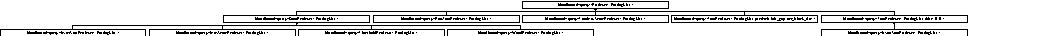
\includegraphics[height=0.484848cm]{classbloodhound_1_1query_1_1Retriever}
\end{center}
\end{figure}
\subsection*{Public Member Functions}
\begin{DoxyCompactItemize}
\item 
virtual std\+::vector$<$ \mbox{\hyperlink{structbloodhound_1_1query_1_1Result}{Result}} $>$ \mbox{\hyperlink{classbloodhound_1_1query_1_1Retriever_ae3c6a4628c5580e620c213b3dcd47c2b}{retrieve}} (const std\+::vector$<$ \mbox{\hyperlink{classbloodhound_1_1PostingList}{Posting\+List}} $>$ \&term\+\_\+postings, const std\+::vector$<$ \mbox{\hyperlink{structbloodhound_1_1Score}{Score}} $>$ \&term\+\_\+weights, std\+::size\+\_\+t k)=0
\begin{DoxyCompactList}\small\item\em Retrieves top-\/k results for the given posting lists and term weights. \end{DoxyCompactList}\item 
virtual nlohmann\+::json \mbox{\hyperlink{classbloodhound_1_1query_1_1Retriever_a58da32a5139b980ba874f8b5e6bb89ec}{stats}} ()
\end{DoxyCompactItemize}


\subsection{Detailed Description}
\subsubsection*{template$<$typename Posting\+List$>$\newline
class bloodhound\+::query\+::\+Retriever$<$ Posting\+List $>$}

A base abstract super-\/class of all document retrievers. 

\subsection{Member Function Documentation}
\mbox{\Hypertarget{classbloodhound_1_1query_1_1Retriever_ae3c6a4628c5580e620c213b3dcd47c2b}\label{classbloodhound_1_1query_1_1Retriever_ae3c6a4628c5580e620c213b3dcd47c2b}} 
\index{bloodhound\+::query\+::\+Retriever@{bloodhound\+::query\+::\+Retriever}!retrieve@{retrieve}}
\index{retrieve@{retrieve}!bloodhound\+::query\+::\+Retriever@{bloodhound\+::query\+::\+Retriever}}
\subsubsection{\texorpdfstring{retrieve()}{retrieve()}}
{\footnotesize\ttfamily template$<$typename Posting\+List $>$ \\
virtual std\+::vector$<$\mbox{\hyperlink{structbloodhound_1_1query_1_1Result}{Result}}$>$ \mbox{\hyperlink{classbloodhound_1_1query_1_1Retriever}{bloodhound\+::query\+::\+Retriever}}$<$ \mbox{\hyperlink{classbloodhound_1_1PostingList}{Posting\+List}} $>$\+::retrieve (\begin{DoxyParamCaption}\item[{const std\+::vector$<$ \mbox{\hyperlink{classbloodhound_1_1PostingList}{Posting\+List}} $>$ \&}]{term\+\_\+postings,  }\item[{const std\+::vector$<$ \mbox{\hyperlink{structbloodhound_1_1Score}{Score}} $>$ \&}]{term\+\_\+weights,  }\item[{std\+::size\+\_\+t}]{k }\end{DoxyParamCaption})\hspace{0.3cm}{\ttfamily [pure virtual]}}



Retrieves top-\/k results for the given posting lists and term weights. 



Implemented in \mbox{\hyperlink{classbloodhound_1_1query_1_1TaatMaxScoreRetriever_af4d96478395b58527969526c3068e7b9}{bloodhound\+::query\+::\+Taat\+Max\+Score\+Retriever$<$ Posting\+List $>$}}, \mbox{\hyperlink{classbloodhound_1_1query_1_1RawTaatRetriever_aafaaf842fdaef297a255e28766af2c0d}{bloodhound\+::query\+::\+Raw\+Taat\+Retriever$<$ Posting\+List $>$}}, \mbox{\hyperlink{classbloodhound_1_1query_1_1TaatRetriever_a58284f19458689021a083c07ea627485}{bloodhound\+::query\+::\+Taat\+Retriever$<$ Posting\+List, prefetch, init\+\_\+gap, acc\+\_\+block\+\_\+size $>$}}, \mbox{\hyperlink{classbloodhound_1_1query_1_1TaatRetriever_a58284f19458689021a083c07ea627485}{bloodhound\+::query\+::\+Taat\+Retriever$<$ Posting\+List, false, 0, 0 $>$}}, \mbox{\hyperlink{classbloodhound_1_1query_1_1WandRetriever_a5f3068bc363c16c5b7255a925ea5af8c}{bloodhound\+::query\+::\+Wand\+Retriever$<$ Posting\+List $>$}}, \mbox{\hyperlink{classbloodhound_1_1query_1_1ThresholdRetriever_a06750450e1246e755ebad2d5dac6e8a8}{bloodhound\+::query\+::\+Threshold\+Retriever$<$ Posting\+List $>$}}, \mbox{\hyperlink{classbloodhound_1_1query_1_1DaatRetriever_ab80b4867fc263827dc2fdbe0965a2e8c}{bloodhound\+::query\+::\+Daat\+Retriever$<$ Posting\+List $>$}}, and \mbox{\hyperlink{classbloodhound_1_1query_1_1ExactSaatRetriever_aced2763cc2a4c12838fef4a20759049e}{bloodhound\+::query\+::\+Exact\+Saat\+Retriever$<$ Posting\+List $>$}}.

\mbox{\Hypertarget{classbloodhound_1_1query_1_1Retriever_a58da32a5139b980ba874f8b5e6bb89ec}\label{classbloodhound_1_1query_1_1Retriever_a58da32a5139b980ba874f8b5e6bb89ec}} 
\index{bloodhound\+::query\+::\+Retriever@{bloodhound\+::query\+::\+Retriever}!stats@{stats}}
\index{stats@{stats}!bloodhound\+::query\+::\+Retriever@{bloodhound\+::query\+::\+Retriever}}
\subsubsection{\texorpdfstring{stats()}{stats()}}
{\footnotesize\ttfamily template$<$typename Posting\+List $>$ \\
virtual nlohmann\+::json \mbox{\hyperlink{classbloodhound_1_1query_1_1Retriever}{bloodhound\+::query\+::\+Retriever}}$<$ \mbox{\hyperlink{classbloodhound_1_1PostingList}{Posting\+List}} $>$\+::stats (\begin{DoxyParamCaption}{ }\end{DoxyParamCaption})\hspace{0.3cm}{\ttfamily [inline]}, {\ttfamily [virtual]}}



Reimplemented in \mbox{\hyperlink{classbloodhound_1_1query_1_1WandRetriever_a1e593c2cddb2ca4f2415c59ca26e6a36}{bloodhound\+::query\+::\+Wand\+Retriever$<$ Posting\+List $>$}}, \mbox{\hyperlink{classbloodhound_1_1query_1_1ThresholdRetriever_aa21e5b44d70bfdf058e5f9c5a1abc008}{bloodhound\+::query\+::\+Threshold\+Retriever$<$ Posting\+List $>$}}, and \mbox{\hyperlink{classbloodhound_1_1query_1_1ExactSaatRetriever_a716838f463f124964e76f48bc37d32cc}{bloodhound\+::query\+::\+Exact\+Saat\+Retriever$<$ Posting\+List $>$}}.



The documentation for this class was generated from the following file\+:\begin{DoxyCompactItemize}
\item 
include/\mbox{\hyperlink{query_8hpp}{query.\+hpp}}\end{DoxyCompactItemize}

\hypertarget{structbloodhound_1_1Score}{}\section{bloodhound\+:\+:Score Struct Reference}
\label{structbloodhound_1_1Score}\index{bloodhound\+::\+Score@{bloodhound\+::\+Score}}


{\ttfamily \#include $<$index.\+hpp$>$}

Inheritance diagram for bloodhound\+:\+:Score\+:\begin{figure}[H]
\begin{center}
\leavevmode
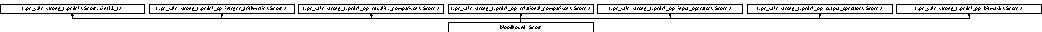
\includegraphics[height=0.427808cm]{structbloodhound_1_1Score}
\end{center}
\end{figure}


The documentation for this struct was generated from the following file\+:\begin{DoxyCompactItemize}
\item 
include/\mbox{\hyperlink{index_8hpp}{index.\+hpp}}\end{DoxyCompactItemize}

\hypertarget{structbloodhound_1_1score__greater}{}\section{bloodhound\+:\+:score\+\_\+greater$<$ Posting $>$ Struct Template Reference}
\label{structbloodhound_1_1score__greater}\index{bloodhound\+::score\+\_\+greater$<$ Posting $>$@{bloodhound\+::score\+\_\+greater$<$ Posting $>$}}


{\ttfamily \#include $<$index.\+hpp$>$}

\subsection*{Public Member Functions}
\begin{DoxyCompactItemize}
\item 
bool \hyperlink{structbloodhound_1_1score__greater_a56a430279ebf5d6b2526335fe3b2d668}{operator()} (const \hyperlink{structbloodhound_1_1Posting}{Posting} \&lhs, const \hyperlink{structbloodhound_1_1Posting}{Posting} \&rhs)
\end{DoxyCompactItemize}


\subsection{Member Function Documentation}
\mbox{\Hypertarget{structbloodhound_1_1score__greater_a56a430279ebf5d6b2526335fe3b2d668}\label{structbloodhound_1_1score__greater_a56a430279ebf5d6b2526335fe3b2d668}} 
\index{bloodhound\+::score\+\_\+greater@{bloodhound\+::score\+\_\+greater}!operator()@{operator()}}
\index{operator()@{operator()}!bloodhound\+::score\+\_\+greater@{bloodhound\+::score\+\_\+greater}}
\subsubsection{\texorpdfstring{operator()()}{operator()()}}
{\footnotesize\ttfamily template$<$class Posting $>$ \\
bool \hyperlink{structbloodhound_1_1score__greater}{bloodhound\+::score\+\_\+greater}$<$ \hyperlink{structbloodhound_1_1Posting}{Posting} $>$\+::operator() (\begin{DoxyParamCaption}\item[{const \hyperlink{structbloodhound_1_1Posting}{Posting} \&}]{lhs,  }\item[{const \hyperlink{structbloodhound_1_1Posting}{Posting} \&}]{rhs }\end{DoxyParamCaption})\hspace{0.3cm}{\ttfamily [inline]}}



The documentation for this struct was generated from the following file\+:\begin{DoxyCompactItemize}
\item 
include/\hyperlink{index_8hpp}{index.\+hpp}\end{DoxyCompactItemize}

\hypertarget{classbloodhound_1_1query_1_1TaatMaxScoreRetriever}{}\section{bloodhound\+:\+:query\+:\+:Taat\+Max\+Score\+Retriever$<$ Posting\+List $>$ Class Template Reference}
\label{classbloodhound_1_1query_1_1TaatMaxScoreRetriever}\index{bloodhound\+::query\+::\+Taat\+Max\+Score\+Retriever$<$ Posting\+List $>$@{bloodhound\+::query\+::\+Taat\+Max\+Score\+Retriever$<$ Posting\+List $>$}}


{\ttfamily \#include $<$retrievers.\+hpp$>$}

Inheritance diagram for bloodhound\+:\+:query\+:\+:Taat\+Max\+Score\+Retriever$<$ Posting\+List $>$\+:\begin{figure}[H]
\begin{center}
\leavevmode
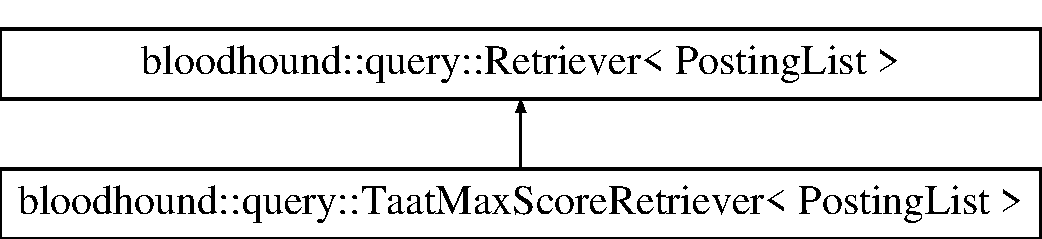
\includegraphics[height=2.000000cm]{classbloodhound_1_1query_1_1TaatMaxScoreRetriever}
\end{center}
\end{figure}
\subsection*{Public Member Functions}
\begin{DoxyCompactItemize}
\item 
\mbox{\hyperlink{classbloodhound_1_1query_1_1TaatMaxScoreRetriever_a8f452aa87a82194bf337e4ce6a06c1f4}{Taat\+Max\+Score\+Retriever}} (std\+::size\+\_\+t collection\+\_\+size)
\item 
std\+::vector$<$ std\+::size\+\_\+t $>$ \mbox{\hyperlink{classbloodhound_1_1query_1_1TaatMaxScoreRetriever_a4c5253dee6541cf173f4f2e16803c702}{sorted\+\_\+by\+\_\+length}} (const std\+::vector$<$ \mbox{\hyperlink{classbloodhound_1_1PostingList}{Posting\+List}} $>$ \&lists\+\_\+for\+\_\+terms)
\item 
virtual std\+::vector$<$ \mbox{\hyperlink{structbloodhound_1_1query_1_1Result}{Result}} $>$ \mbox{\hyperlink{classbloodhound_1_1query_1_1TaatMaxScoreRetriever_af4d96478395b58527969526c3068e7b9}{retrieve}} (const std\+::vector$<$ \mbox{\hyperlink{classbloodhound_1_1PostingList}{Posting\+List}} $>$ \&lists\+\_\+for\+\_\+terms, const std\+::vector$<$ \mbox{\hyperlink{structbloodhound_1_1Score}{Score}} $>$ \&term\+\_\+weights, std\+::size\+\_\+t k)
\begin{DoxyCompactList}\small\item\em Retrieves top-\/k results for the given posting lists and term weights. \end{DoxyCompactList}\end{DoxyCompactItemize}


\subsection{Constructor \& Destructor Documentation}
\mbox{\Hypertarget{classbloodhound_1_1query_1_1TaatMaxScoreRetriever_a8f452aa87a82194bf337e4ce6a06c1f4}\label{classbloodhound_1_1query_1_1TaatMaxScoreRetriever_a8f452aa87a82194bf337e4ce6a06c1f4}} 
\index{bloodhound\+::query\+::\+Taat\+Max\+Score\+Retriever@{bloodhound\+::query\+::\+Taat\+Max\+Score\+Retriever}!Taat\+Max\+Score\+Retriever@{Taat\+Max\+Score\+Retriever}}
\index{Taat\+Max\+Score\+Retriever@{Taat\+Max\+Score\+Retriever}!bloodhound\+::query\+::\+Taat\+Max\+Score\+Retriever@{bloodhound\+::query\+::\+Taat\+Max\+Score\+Retriever}}
\subsubsection{\texorpdfstring{Taat\+Max\+Score\+Retriever()}{TaatMaxScoreRetriever()}}
{\footnotesize\ttfamily template$<$typename Posting\+List $>$ \\
\mbox{\hyperlink{classbloodhound_1_1query_1_1TaatMaxScoreRetriever}{bloodhound\+::query\+::\+Taat\+Max\+Score\+Retriever}}$<$ \mbox{\hyperlink{classbloodhound_1_1PostingList}{Posting\+List}} $>$\+::\mbox{\hyperlink{classbloodhound_1_1query_1_1TaatMaxScoreRetriever}{Taat\+Max\+Score\+Retriever}} (\begin{DoxyParamCaption}\item[{std\+::size\+\_\+t}]{collection\+\_\+size }\end{DoxyParamCaption})\hspace{0.3cm}{\ttfamily [inline]}}



\subsection{Member Function Documentation}
\mbox{\Hypertarget{classbloodhound_1_1query_1_1TaatMaxScoreRetriever_af4d96478395b58527969526c3068e7b9}\label{classbloodhound_1_1query_1_1TaatMaxScoreRetriever_af4d96478395b58527969526c3068e7b9}} 
\index{bloodhound\+::query\+::\+Taat\+Max\+Score\+Retriever@{bloodhound\+::query\+::\+Taat\+Max\+Score\+Retriever}!retrieve@{retrieve}}
\index{retrieve@{retrieve}!bloodhound\+::query\+::\+Taat\+Max\+Score\+Retriever@{bloodhound\+::query\+::\+Taat\+Max\+Score\+Retriever}}
\subsubsection{\texorpdfstring{retrieve()}{retrieve()}}
{\footnotesize\ttfamily template$<$typename Posting\+List $>$ \\
virtual std\+::vector$<$\mbox{\hyperlink{structbloodhound_1_1query_1_1Result}{Result}}$>$ \mbox{\hyperlink{classbloodhound_1_1query_1_1TaatMaxScoreRetriever}{bloodhound\+::query\+::\+Taat\+Max\+Score\+Retriever}}$<$ \mbox{\hyperlink{classbloodhound_1_1PostingList}{Posting\+List}} $>$\+::retrieve (\begin{DoxyParamCaption}\item[{const std\+::vector$<$ \mbox{\hyperlink{classbloodhound_1_1PostingList}{Posting\+List}} $>$ \&}]{term\+\_\+postings,  }\item[{const std\+::vector$<$ \mbox{\hyperlink{structbloodhound_1_1Score}{Score}} $>$ \&}]{term\+\_\+weights,  }\item[{std\+::size\+\_\+t}]{k }\end{DoxyParamCaption})\hspace{0.3cm}{\ttfamily [inline]}, {\ttfamily [virtual]}}



Retrieves top-\/k results for the given posting lists and term weights. 



Implements \mbox{\hyperlink{classbloodhound_1_1query_1_1Retriever_ae3c6a4628c5580e620c213b3dcd47c2b}{bloodhound\+::query\+::\+Retriever$<$ Posting\+List $>$}}.

\mbox{\Hypertarget{classbloodhound_1_1query_1_1TaatMaxScoreRetriever_a4c5253dee6541cf173f4f2e16803c702}\label{classbloodhound_1_1query_1_1TaatMaxScoreRetriever_a4c5253dee6541cf173f4f2e16803c702}} 
\index{bloodhound\+::query\+::\+Taat\+Max\+Score\+Retriever@{bloodhound\+::query\+::\+Taat\+Max\+Score\+Retriever}!sorted\+\_\+by\+\_\+length@{sorted\+\_\+by\+\_\+length}}
\index{sorted\+\_\+by\+\_\+length@{sorted\+\_\+by\+\_\+length}!bloodhound\+::query\+::\+Taat\+Max\+Score\+Retriever@{bloodhound\+::query\+::\+Taat\+Max\+Score\+Retriever}}
\subsubsection{\texorpdfstring{sorted\+\_\+by\+\_\+length()}{sorted\_by\_length()}}
{\footnotesize\ttfamily template$<$typename Posting\+List $>$ \\
std\+::vector$<$std\+::size\+\_\+t$>$ \mbox{\hyperlink{classbloodhound_1_1query_1_1TaatMaxScoreRetriever}{bloodhound\+::query\+::\+Taat\+Max\+Score\+Retriever}}$<$ \mbox{\hyperlink{classbloodhound_1_1PostingList}{Posting\+List}} $>$\+::sorted\+\_\+by\+\_\+length (\begin{DoxyParamCaption}\item[{const std\+::vector$<$ \mbox{\hyperlink{classbloodhound_1_1PostingList}{Posting\+List}} $>$ \&}]{lists\+\_\+for\+\_\+terms }\end{DoxyParamCaption})\hspace{0.3cm}{\ttfamily [inline]}}



The documentation for this class was generated from the following file\+:\begin{DoxyCompactItemize}
\item 
include/\mbox{\hyperlink{retrievers_8hpp}{retrievers.\+hpp}}\end{DoxyCompactItemize}

\hypertarget{classbloodhound_1_1query_1_1TaatRetriever}{}\section{bloodhound\+:\+:query\+:\+:Taat\+Retriever$<$ Posting\+List, prefetch, init\+\_\+gap, acc\+\_\+block\+\_\+size $>$ Class Template Reference}
\label{classbloodhound_1_1query_1_1TaatRetriever}\index{bloodhound\+::query\+::\+Taat\+Retriever$<$ Posting\+List, prefetch, init\+\_\+gap, acc\+\_\+block\+\_\+size $>$@{bloodhound\+::query\+::\+Taat\+Retriever$<$ Posting\+List, prefetch, init\+\_\+gap, acc\+\_\+block\+\_\+size $>$}}


{\ttfamily \#include $<$retrievers.\+hpp$>$}

Inheritance diagram for bloodhound\+:\+:query\+:\+:Taat\+Retriever$<$ Posting\+List, prefetch, init\+\_\+gap, acc\+\_\+block\+\_\+size $>$\+:\begin{figure}[H]
\begin{center}
\leavevmode
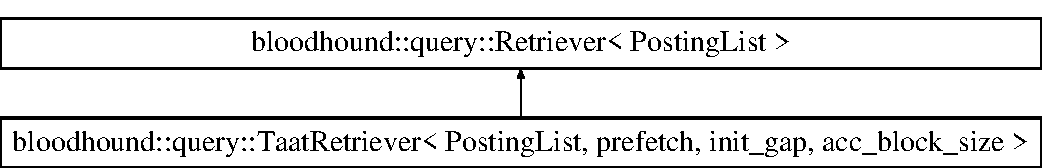
\includegraphics[height=2.000000cm]{classbloodhound_1_1query_1_1TaatRetriever}
\end{center}
\end{figure}
\subsection*{Public Member Functions}
\begin{DoxyCompactItemize}
\item 
\hyperlink{classbloodhound_1_1query_1_1TaatRetriever_af443da08f4200fb84a3481d47bc4ac35}{Taat\+Retriever} (std\+::size\+\_\+t collection\+\_\+size)
\begin{DoxyCompactList}\small\item\em Constructs a \hyperlink{classbloodhound_1_1query_1_1TaatRetriever}{Taat\+Retriever} with an accumulator array of collection\+\_\+size. \end{DoxyCompactList}\item 
void \hyperlink{classbloodhound_1_1query_1_1TaatRetriever_a34def8d627b446d7459792ab9c50dcab}{accumulate\+\_\+posting} (\hyperlink{structbloodhound_1_1Doc}{Doc} doc, \hyperlink{structbloodhound_1_1Score}{Score} score\+\_\+delta, std\+::vector$<$ \hyperlink{structbloodhound_1_1Score}{Score} $>$ \&acc)
\begin{DoxyCompactList}\small\item\em Accumulates the posting that is being processed. \end{DoxyCompactList}\item 
void \hyperlink{classbloodhound_1_1query_1_1TaatRetriever_a1b476e4ada85862cb79a92b6424d2aa2}{traverse} (const std\+::vector$<$ \hyperlink{classbloodhound_1_1PostingList}{Posting\+List} $>$ \&lists\+\_\+for\+\_\+terms, const std\+::vector$<$ \hyperlink{structbloodhound_1_1Score}{Score} $>$ \&term\+\_\+weights)
\begin{DoxyCompactList}\small\item\em Traverses a single posting lists and accumulates its scores. \end{DoxyCompactList}\item 
\hyperlink{structbloodhound_1_1Score}{Score} \hyperlink{classbloodhound_1_1query_1_1TaatRetriever_ae1c8d9643ca85ba7dba32325538e30b5}{score\+\_\+of} (\hyperlink{structbloodhound_1_1Doc}{Doc} doc) const
\begin{DoxyCompactList}\small\item\em Returns the accumulated score of doc. \end{DoxyCompactList}\item 
std\+::vector$<$ \hyperlink{structbloodhound_1_1query_1_1Result}{Result} $>$ \hyperlink{classbloodhound_1_1query_1_1TaatRetriever_a7f631f87075249c768873d15a59956c5}{aggregate\+\_\+top} (std\+::size\+\_\+t k)
\item 
void \hyperlink{classbloodhound_1_1query_1_1TaatRetriever_a6fedf448e3d9394ecaa787bf60a9cb84}{clear\+\_\+accumulator\+\_\+array} ()
\begin{DoxyCompactList}\small\item\em Fill the accumulator array with zeroes. \end{DoxyCompactList}\item 
void \hyperlink{classbloodhound_1_1query_1_1TaatRetriever_a00a64711e5d865ba4c53e3accdb61d3f}{clear\+\_\+blocks} ()
\begin{DoxyCompactList}\small\item\em Set all block maximum scores with zeroes. \end{DoxyCompactList}\item 
void \hyperlink{classbloodhound_1_1query_1_1TaatRetriever_ad6739ab7025c6de9e65945cff25c55b4}{next\+\_\+query} ()
\item 
virtual std\+::vector$<$ \hyperlink{structbloodhound_1_1query_1_1Result}{Result} $>$ \hyperlink{classbloodhound_1_1query_1_1TaatRetriever_a58284f19458689021a083c07ea627485}{retrieve} (const std\+::vector$<$ \hyperlink{classbloodhound_1_1PostingList}{Posting\+List} $>$ \&lists\+\_\+for\+\_\+terms, const std\+::vector$<$ \hyperlink{structbloodhound_1_1Score}{Score} $>$ \&term\+\_\+weights, std\+::size\+\_\+t k)
\begin{DoxyCompactList}\small\item\em Retrieves top-\/k results for the given posting lists and term weights. \end{DoxyCompactList}\end{DoxyCompactItemize}
\subsection*{Protected Attributes}
\begin{DoxyCompactItemize}
\item 
\hyperlink{namespacebloodhound_1_1query_aa67214af106292b2483995adea986b08}{Query\+Id} \hyperlink{classbloodhound_1_1query_1_1TaatRetriever_aa9a1b8ca0cb570bcffe6b6c68e8c2e20}{query\+\_\+id}
\item 
\hyperlink{structbloodhound_1_1Score}{Score} \hyperlink{classbloodhound_1_1query_1_1TaatRetriever_aa27d16b326df60affe26e005f9abb4f6}{qidx\+\_\+shifted}
\item 
\hyperlink{structbloodhound_1_1Score}{Score} \hyperlink{classbloodhound_1_1query_1_1TaatRetriever_ac38b873ceff34b55bb8ac82800946825}{score\+\_\+mask}
\item 
unsigned int \hyperlink{classbloodhound_1_1query_1_1TaatRetriever_aa2b4875de4f02a856e64560bf002296f}{bits\+\_\+to\+\_\+shift}
\item 
std\+::vector$<$ \hyperlink{structbloodhound_1_1Score}{Score} $>$ \hyperlink{classbloodhound_1_1query_1_1TaatRetriever_a604c7ab279ced03ccc1866d55c844b11}{accumulator\+\_\+array}
\begin{DoxyCompactList}\small\item\em The array of accumulated values for each document. \end{DoxyCompactList}\item 
std\+::vector$<$ \hyperlink{structbloodhound_1_1Score}{Score} $>$ \hyperlink{classbloodhound_1_1query_1_1TaatRetriever_ac870574844dc3be6c40cf1236e1ff6cc}{block\+\_\+max\+\_\+scores}
\item 
std\+::size\+\_\+t \hyperlink{classbloodhound_1_1query_1_1TaatRetriever_a87786d9af7993da498d60304eab245cf}{nblocks}
\end{DoxyCompactItemize}


\subsection{Detailed Description}
\subsubsection*{template$<$typename Posting\+List, bool prefetch = false, unsigned short init\+\_\+gap = 0, unsigned int acc\+\_\+block\+\_\+size = 0$>$\newline
class bloodhound\+::query\+::\+Taat\+Retriever$<$ Posting\+List, prefetch, init\+\_\+gap, acc\+\_\+block\+\_\+size $>$}

Term-\/at-\/a-\/time document retriever.

\hyperlink{classbloodhound_1_1PostingList}{Posting\+List} requires\+:
\begin{DoxyItemize}
\item doc\+\_\+begin() and doc\+\_\+end()\+: document start and end iterator, respectively;
\item score\+\_\+begin() and score\+\_\+end()\+: score start and end iterator, respectively;
\item length()\+: posting list length; 
\end{DoxyItemize}

\subsection{Constructor \& Destructor Documentation}
\mbox{\Hypertarget{classbloodhound_1_1query_1_1TaatRetriever_af443da08f4200fb84a3481d47bc4ac35}\label{classbloodhound_1_1query_1_1TaatRetriever_af443da08f4200fb84a3481d47bc4ac35}} 
\index{bloodhound\+::query\+::\+Taat\+Retriever@{bloodhound\+::query\+::\+Taat\+Retriever}!Taat\+Retriever@{Taat\+Retriever}}
\index{Taat\+Retriever@{Taat\+Retriever}!bloodhound\+::query\+::\+Taat\+Retriever@{bloodhound\+::query\+::\+Taat\+Retriever}}
\subsubsection{\texorpdfstring{Taat\+Retriever()}{TaatRetriever()}}
{\footnotesize\ttfamily template$<$typename Posting\+List, bool prefetch = false, unsigned short init\+\_\+gap = 0, unsigned int acc\+\_\+block\+\_\+size = 0$>$ \\
\hyperlink{classbloodhound_1_1query_1_1TaatRetriever}{bloodhound\+::query\+::\+Taat\+Retriever}$<$ \hyperlink{classbloodhound_1_1PostingList}{Posting\+List}, prefetch, init\+\_\+gap, acc\+\_\+block\+\_\+size $>$\+::\hyperlink{classbloodhound_1_1query_1_1TaatRetriever}{Taat\+Retriever} (\begin{DoxyParamCaption}\item[{std\+::size\+\_\+t}]{collection\+\_\+size }\end{DoxyParamCaption})\hspace{0.3cm}{\ttfamily [inline]}}



Constructs a \hyperlink{classbloodhound_1_1query_1_1TaatRetriever}{Taat\+Retriever} with an accumulator array of collection\+\_\+size. 



\subsection{Member Function Documentation}
\mbox{\Hypertarget{classbloodhound_1_1query_1_1TaatRetriever_a34def8d627b446d7459792ab9c50dcab}\label{classbloodhound_1_1query_1_1TaatRetriever_a34def8d627b446d7459792ab9c50dcab}} 
\index{bloodhound\+::query\+::\+Taat\+Retriever@{bloodhound\+::query\+::\+Taat\+Retriever}!accumulate\+\_\+posting@{accumulate\+\_\+posting}}
\index{accumulate\+\_\+posting@{accumulate\+\_\+posting}!bloodhound\+::query\+::\+Taat\+Retriever@{bloodhound\+::query\+::\+Taat\+Retriever}}
\subsubsection{\texorpdfstring{accumulate\+\_\+posting()}{accumulate\_posting()}}
{\footnotesize\ttfamily template$<$typename Posting\+List, bool prefetch = false, unsigned short init\+\_\+gap = 0, unsigned int acc\+\_\+block\+\_\+size = 0$>$ \\
void \hyperlink{classbloodhound_1_1query_1_1TaatRetriever}{bloodhound\+::query\+::\+Taat\+Retriever}$<$ \hyperlink{classbloodhound_1_1PostingList}{Posting\+List}, prefetch, init\+\_\+gap, acc\+\_\+block\+\_\+size $>$\+::accumulate\+\_\+posting (\begin{DoxyParamCaption}\item[{\hyperlink{structbloodhound_1_1Doc}{Doc}}]{doc,  }\item[{\hyperlink{structbloodhound_1_1Score}{Score}}]{score\+\_\+delta,  }\item[{std\+::vector$<$ \hyperlink{structbloodhound_1_1Score}{Score} $>$ \&}]{acc }\end{DoxyParamCaption})\hspace{0.3cm}{\ttfamily [inline]}}



Accumulates the posting that is being processed. 

\mbox{\Hypertarget{classbloodhound_1_1query_1_1TaatRetriever_a7f631f87075249c768873d15a59956c5}\label{classbloodhound_1_1query_1_1TaatRetriever_a7f631f87075249c768873d15a59956c5}} 
\index{bloodhound\+::query\+::\+Taat\+Retriever@{bloodhound\+::query\+::\+Taat\+Retriever}!aggregate\+\_\+top@{aggregate\+\_\+top}}
\index{aggregate\+\_\+top@{aggregate\+\_\+top}!bloodhound\+::query\+::\+Taat\+Retriever@{bloodhound\+::query\+::\+Taat\+Retriever}}
\subsubsection{\texorpdfstring{aggregate\+\_\+top()}{aggregate\_top()}}
{\footnotesize\ttfamily template$<$typename Posting\+List, bool prefetch = false, unsigned short init\+\_\+gap = 0, unsigned int acc\+\_\+block\+\_\+size = 0$>$ \\
std\+::vector$<$\hyperlink{structbloodhound_1_1query_1_1Result}{Result}$>$ \hyperlink{classbloodhound_1_1query_1_1TaatRetriever}{bloodhound\+::query\+::\+Taat\+Retriever}$<$ \hyperlink{classbloodhound_1_1PostingList}{Posting\+List}, prefetch, init\+\_\+gap, acc\+\_\+block\+\_\+size $>$\+::aggregate\+\_\+top (\begin{DoxyParamCaption}\item[{std\+::size\+\_\+t}]{k }\end{DoxyParamCaption})\hspace{0.3cm}{\ttfamily [inline]}}

Returns the top-\/k highest ranked documents.

It may return fewer documents if fewer of them contain any term. \mbox{\Hypertarget{classbloodhound_1_1query_1_1TaatRetriever_a6fedf448e3d9394ecaa787bf60a9cb84}\label{classbloodhound_1_1query_1_1TaatRetriever_a6fedf448e3d9394ecaa787bf60a9cb84}} 
\index{bloodhound\+::query\+::\+Taat\+Retriever@{bloodhound\+::query\+::\+Taat\+Retriever}!clear\+\_\+accumulator\+\_\+array@{clear\+\_\+accumulator\+\_\+array}}
\index{clear\+\_\+accumulator\+\_\+array@{clear\+\_\+accumulator\+\_\+array}!bloodhound\+::query\+::\+Taat\+Retriever@{bloodhound\+::query\+::\+Taat\+Retriever}}
\subsubsection{\texorpdfstring{clear\+\_\+accumulator\+\_\+array()}{clear\_accumulator\_array()}}
{\footnotesize\ttfamily template$<$typename Posting\+List, bool prefetch = false, unsigned short init\+\_\+gap = 0, unsigned int acc\+\_\+block\+\_\+size = 0$>$ \\
void \hyperlink{classbloodhound_1_1query_1_1TaatRetriever}{bloodhound\+::query\+::\+Taat\+Retriever}$<$ \hyperlink{classbloodhound_1_1PostingList}{Posting\+List}, prefetch, init\+\_\+gap, acc\+\_\+block\+\_\+size $>$\+::clear\+\_\+accumulator\+\_\+array (\begin{DoxyParamCaption}{ }\end{DoxyParamCaption})\hspace{0.3cm}{\ttfamily [inline]}}



Fill the accumulator array with zeroes. 

\mbox{\Hypertarget{classbloodhound_1_1query_1_1TaatRetriever_a00a64711e5d865ba4c53e3accdb61d3f}\label{classbloodhound_1_1query_1_1TaatRetriever_a00a64711e5d865ba4c53e3accdb61d3f}} 
\index{bloodhound\+::query\+::\+Taat\+Retriever@{bloodhound\+::query\+::\+Taat\+Retriever}!clear\+\_\+blocks@{clear\+\_\+blocks}}
\index{clear\+\_\+blocks@{clear\+\_\+blocks}!bloodhound\+::query\+::\+Taat\+Retriever@{bloodhound\+::query\+::\+Taat\+Retriever}}
\subsubsection{\texorpdfstring{clear\+\_\+blocks()}{clear\_blocks()}}
{\footnotesize\ttfamily template$<$typename Posting\+List, bool prefetch = false, unsigned short init\+\_\+gap = 0, unsigned int acc\+\_\+block\+\_\+size = 0$>$ \\
void \hyperlink{classbloodhound_1_1query_1_1TaatRetriever}{bloodhound\+::query\+::\+Taat\+Retriever}$<$ \hyperlink{classbloodhound_1_1PostingList}{Posting\+List}, prefetch, init\+\_\+gap, acc\+\_\+block\+\_\+size $>$\+::clear\+\_\+blocks (\begin{DoxyParamCaption}{ }\end{DoxyParamCaption})\hspace{0.3cm}{\ttfamily [inline]}}



Set all block maximum scores with zeroes. 

\mbox{\Hypertarget{classbloodhound_1_1query_1_1TaatRetriever_ad6739ab7025c6de9e65945cff25c55b4}\label{classbloodhound_1_1query_1_1TaatRetriever_ad6739ab7025c6de9e65945cff25c55b4}} 
\index{bloodhound\+::query\+::\+Taat\+Retriever@{bloodhound\+::query\+::\+Taat\+Retriever}!next\+\_\+query@{next\+\_\+query}}
\index{next\+\_\+query@{next\+\_\+query}!bloodhound\+::query\+::\+Taat\+Retriever@{bloodhound\+::query\+::\+Taat\+Retriever}}
\subsubsection{\texorpdfstring{next\+\_\+query()}{next\_query()}}
{\footnotesize\ttfamily template$<$typename Posting\+List, bool prefetch = false, unsigned short init\+\_\+gap = 0, unsigned int acc\+\_\+block\+\_\+size = 0$>$ \\
void \hyperlink{classbloodhound_1_1query_1_1TaatRetriever}{bloodhound\+::query\+::\+Taat\+Retriever}$<$ \hyperlink{classbloodhound_1_1PostingList}{Posting\+List}, prefetch, init\+\_\+gap, acc\+\_\+block\+\_\+size $>$\+::next\+\_\+query (\begin{DoxyParamCaption}{ }\end{DoxyParamCaption})\hspace{0.3cm}{\ttfamily [inline]}}

Proceed to the next query.

Clears the accumulators if necessary and keeps track of the query I\+Ds. \mbox{\Hypertarget{classbloodhound_1_1query_1_1TaatRetriever_a58284f19458689021a083c07ea627485}\label{classbloodhound_1_1query_1_1TaatRetriever_a58284f19458689021a083c07ea627485}} 
\index{bloodhound\+::query\+::\+Taat\+Retriever@{bloodhound\+::query\+::\+Taat\+Retriever}!retrieve@{retrieve}}
\index{retrieve@{retrieve}!bloodhound\+::query\+::\+Taat\+Retriever@{bloodhound\+::query\+::\+Taat\+Retriever}}
\subsubsection{\texorpdfstring{retrieve()}{retrieve()}}
{\footnotesize\ttfamily template$<$typename Posting\+List, bool prefetch = false, unsigned short init\+\_\+gap = 0, unsigned int acc\+\_\+block\+\_\+size = 0$>$ \\
virtual std\+::vector$<$\hyperlink{structbloodhound_1_1query_1_1Result}{Result}$>$ \hyperlink{classbloodhound_1_1query_1_1TaatRetriever}{bloodhound\+::query\+::\+Taat\+Retriever}$<$ \hyperlink{classbloodhound_1_1PostingList}{Posting\+List}, prefetch, init\+\_\+gap, acc\+\_\+block\+\_\+size $>$\+::retrieve (\begin{DoxyParamCaption}\item[{const std\+::vector$<$ \hyperlink{classbloodhound_1_1PostingList}{Posting\+List} $>$ \&}]{term\+\_\+postings,  }\item[{const std\+::vector$<$ \hyperlink{structbloodhound_1_1Score}{Score} $>$ \&}]{term\+\_\+weights,  }\item[{std\+::size\+\_\+t}]{k }\end{DoxyParamCaption})\hspace{0.3cm}{\ttfamily [inline]}, {\ttfamily [virtual]}}



Retrieves top-\/k results for the given posting lists and term weights. 



Implements \hyperlink{classbloodhound_1_1query_1_1Retriever_ae3c6a4628c5580e620c213b3dcd47c2b}{bloodhound\+::query\+::\+Retriever$<$ Posting\+List $>$}.



Reimplemented in \hyperlink{classbloodhound_1_1query_1_1ExactSaatRetriever_aced2763cc2a4c12838fef4a20759049e}{bloodhound\+::query\+::\+Exact\+Saat\+Retriever$<$ Posting\+List $>$}.

\mbox{\Hypertarget{classbloodhound_1_1query_1_1TaatRetriever_ae1c8d9643ca85ba7dba32325538e30b5}\label{classbloodhound_1_1query_1_1TaatRetriever_ae1c8d9643ca85ba7dba32325538e30b5}} 
\index{bloodhound\+::query\+::\+Taat\+Retriever@{bloodhound\+::query\+::\+Taat\+Retriever}!score\+\_\+of@{score\+\_\+of}}
\index{score\+\_\+of@{score\+\_\+of}!bloodhound\+::query\+::\+Taat\+Retriever@{bloodhound\+::query\+::\+Taat\+Retriever}}
\subsubsection{\texorpdfstring{score\+\_\+of()}{score\_of()}}
{\footnotesize\ttfamily template$<$typename Posting\+List, bool prefetch = false, unsigned short init\+\_\+gap = 0, unsigned int acc\+\_\+block\+\_\+size = 0$>$ \\
\hyperlink{structbloodhound_1_1Score}{Score} \hyperlink{classbloodhound_1_1query_1_1TaatRetriever}{bloodhound\+::query\+::\+Taat\+Retriever}$<$ \hyperlink{classbloodhound_1_1PostingList}{Posting\+List}, prefetch, init\+\_\+gap, acc\+\_\+block\+\_\+size $>$\+::score\+\_\+of (\begin{DoxyParamCaption}\item[{\hyperlink{structbloodhound_1_1Doc}{Doc}}]{doc }\end{DoxyParamCaption}) const\hspace{0.3cm}{\ttfamily [inline]}}



Returns the accumulated score of doc. 

\mbox{\Hypertarget{classbloodhound_1_1query_1_1TaatRetriever_a1b476e4ada85862cb79a92b6424d2aa2}\label{classbloodhound_1_1query_1_1TaatRetriever_a1b476e4ada85862cb79a92b6424d2aa2}} 
\index{bloodhound\+::query\+::\+Taat\+Retriever@{bloodhound\+::query\+::\+Taat\+Retriever}!traverse@{traverse}}
\index{traverse@{traverse}!bloodhound\+::query\+::\+Taat\+Retriever@{bloodhound\+::query\+::\+Taat\+Retriever}}
\subsubsection{\texorpdfstring{traverse()}{traverse()}}
{\footnotesize\ttfamily template$<$typename Posting\+List, bool prefetch = false, unsigned short init\+\_\+gap = 0, unsigned int acc\+\_\+block\+\_\+size = 0$>$ \\
void \hyperlink{classbloodhound_1_1query_1_1TaatRetriever}{bloodhound\+::query\+::\+Taat\+Retriever}$<$ \hyperlink{classbloodhound_1_1PostingList}{Posting\+List}, prefetch, init\+\_\+gap, acc\+\_\+block\+\_\+size $>$\+::traverse (\begin{DoxyParamCaption}\item[{const std\+::vector$<$ \hyperlink{classbloodhound_1_1PostingList}{Posting\+List} $>$ \&}]{lists\+\_\+for\+\_\+terms,  }\item[{const std\+::vector$<$ \hyperlink{structbloodhound_1_1Score}{Score} $>$ \&}]{term\+\_\+weights }\end{DoxyParamCaption})\hspace{0.3cm}{\ttfamily [inline]}}



Traverses a single posting lists and accumulates its scores. 

Traverses the postings and accumulates the scores. 

\subsection{Member Data Documentation}
\mbox{\Hypertarget{classbloodhound_1_1query_1_1TaatRetriever_a604c7ab279ced03ccc1866d55c844b11}\label{classbloodhound_1_1query_1_1TaatRetriever_a604c7ab279ced03ccc1866d55c844b11}} 
\index{bloodhound\+::query\+::\+Taat\+Retriever@{bloodhound\+::query\+::\+Taat\+Retriever}!accumulator\+\_\+array@{accumulator\+\_\+array}}
\index{accumulator\+\_\+array@{accumulator\+\_\+array}!bloodhound\+::query\+::\+Taat\+Retriever@{bloodhound\+::query\+::\+Taat\+Retriever}}
\subsubsection{\texorpdfstring{accumulator\+\_\+array}{accumulator\_array}}
{\footnotesize\ttfamily template$<$typename Posting\+List, bool prefetch = false, unsigned short init\+\_\+gap = 0, unsigned int acc\+\_\+block\+\_\+size = 0$>$ \\
std\+::vector$<$\hyperlink{structbloodhound_1_1Score}{Score}$>$ \hyperlink{classbloodhound_1_1query_1_1TaatRetriever}{bloodhound\+::query\+::\+Taat\+Retriever}$<$ \hyperlink{classbloodhound_1_1PostingList}{Posting\+List}, prefetch, init\+\_\+gap, acc\+\_\+block\+\_\+size $>$\+::accumulator\+\_\+array\hspace{0.3cm}{\ttfamily [protected]}}



The array of accumulated values for each document. 

\mbox{\Hypertarget{classbloodhound_1_1query_1_1TaatRetriever_aa2b4875de4f02a856e64560bf002296f}\label{classbloodhound_1_1query_1_1TaatRetriever_aa2b4875de4f02a856e64560bf002296f}} 
\index{bloodhound\+::query\+::\+Taat\+Retriever@{bloodhound\+::query\+::\+Taat\+Retriever}!bits\+\_\+to\+\_\+shift@{bits\+\_\+to\+\_\+shift}}
\index{bits\+\_\+to\+\_\+shift@{bits\+\_\+to\+\_\+shift}!bloodhound\+::query\+::\+Taat\+Retriever@{bloodhound\+::query\+::\+Taat\+Retriever}}
\subsubsection{\texorpdfstring{bits\+\_\+to\+\_\+shift}{bits\_to\_shift}}
{\footnotesize\ttfamily template$<$typename Posting\+List, bool prefetch = false, unsigned short init\+\_\+gap = 0, unsigned int acc\+\_\+block\+\_\+size = 0$>$ \\
unsigned int \hyperlink{classbloodhound_1_1query_1_1TaatRetriever}{bloodhound\+::query\+::\+Taat\+Retriever}$<$ \hyperlink{classbloodhound_1_1PostingList}{Posting\+List}, prefetch, init\+\_\+gap, acc\+\_\+block\+\_\+size $>$\+::bits\+\_\+to\+\_\+shift\hspace{0.3cm}{\ttfamily [protected]}}

How many bits are used for the score value. This is only used when init\+\_\+gap $>$ 1. \mbox{\Hypertarget{classbloodhound_1_1query_1_1TaatRetriever_ac870574844dc3be6c40cf1236e1ff6cc}\label{classbloodhound_1_1query_1_1TaatRetriever_ac870574844dc3be6c40cf1236e1ff6cc}} 
\index{bloodhound\+::query\+::\+Taat\+Retriever@{bloodhound\+::query\+::\+Taat\+Retriever}!block\+\_\+max\+\_\+scores@{block\+\_\+max\+\_\+scores}}
\index{block\+\_\+max\+\_\+scores@{block\+\_\+max\+\_\+scores}!bloodhound\+::query\+::\+Taat\+Retriever@{bloodhound\+::query\+::\+Taat\+Retriever}}
\subsubsection{\texorpdfstring{block\+\_\+max\+\_\+scores}{block\_max\_scores}}
{\footnotesize\ttfamily template$<$typename Posting\+List, bool prefetch = false, unsigned short init\+\_\+gap = 0, unsigned int acc\+\_\+block\+\_\+size = 0$>$ \\
std\+::vector$<$\hyperlink{structbloodhound_1_1Score}{Score}$>$ \hyperlink{classbloodhound_1_1query_1_1TaatRetriever}{bloodhound\+::query\+::\+Taat\+Retriever}$<$ \hyperlink{classbloodhound_1_1PostingList}{Posting\+List}, prefetch, init\+\_\+gap, acc\+\_\+block\+\_\+size $>$\+::block\+\_\+max\+\_\+scores\hspace{0.3cm}{\ttfamily [protected]}}

Maximum scores for each accumulator block. Only used when acc\+\_\+block\+\_\+size $>$ 0. \mbox{\Hypertarget{classbloodhound_1_1query_1_1TaatRetriever_a87786d9af7993da498d60304eab245cf}\label{classbloodhound_1_1query_1_1TaatRetriever_a87786d9af7993da498d60304eab245cf}} 
\index{bloodhound\+::query\+::\+Taat\+Retriever@{bloodhound\+::query\+::\+Taat\+Retriever}!nblocks@{nblocks}}
\index{nblocks@{nblocks}!bloodhound\+::query\+::\+Taat\+Retriever@{bloodhound\+::query\+::\+Taat\+Retriever}}
\subsubsection{\texorpdfstring{nblocks}{nblocks}}
{\footnotesize\ttfamily template$<$typename Posting\+List, bool prefetch = false, unsigned short init\+\_\+gap = 0, unsigned int acc\+\_\+block\+\_\+size = 0$>$ \\
std\+::size\+\_\+t \hyperlink{classbloodhound_1_1query_1_1TaatRetriever}{bloodhound\+::query\+::\+Taat\+Retriever}$<$ \hyperlink{classbloodhound_1_1PostingList}{Posting\+List}, prefetch, init\+\_\+gap, acc\+\_\+block\+\_\+size $>$\+::nblocks\hspace{0.3cm}{\ttfamily [protected]}}

The number of blocks, calculated based on acc\+\_\+block\+\_\+size and the number of documents in the index. Only used when acc\+\_\+block\+\_\+size $>$ 0. \mbox{\Hypertarget{classbloodhound_1_1query_1_1TaatRetriever_aa27d16b326df60affe26e005f9abb4f6}\label{classbloodhound_1_1query_1_1TaatRetriever_aa27d16b326df60affe26e005f9abb4f6}} 
\index{bloodhound\+::query\+::\+Taat\+Retriever@{bloodhound\+::query\+::\+Taat\+Retriever}!qidx\+\_\+shifted@{qidx\+\_\+shifted}}
\index{qidx\+\_\+shifted@{qidx\+\_\+shifted}!bloodhound\+::query\+::\+Taat\+Retriever@{bloodhound\+::query\+::\+Taat\+Retriever}}
\subsubsection{\texorpdfstring{qidx\+\_\+shifted}{qidx\_shifted}}
{\footnotesize\ttfamily template$<$typename Posting\+List, bool prefetch = false, unsigned short init\+\_\+gap = 0, unsigned int acc\+\_\+block\+\_\+size = 0$>$ \\
\hyperlink{structbloodhound_1_1Score}{Score} \hyperlink{classbloodhound_1_1query_1_1TaatRetriever}{bloodhound\+::query\+::\+Taat\+Retriever}$<$ \hyperlink{classbloodhound_1_1PostingList}{Posting\+List}, prefetch, init\+\_\+gap, acc\+\_\+block\+\_\+size $>$\+::qidx\+\_\+shifted\hspace{0.3cm}{\ttfamily [protected]}}

This is query\+\_\+id shifted to the far left for quick comparison of the accumulated values. This is only used when init\+\_\+gap $>$ 1. \mbox{\Hypertarget{classbloodhound_1_1query_1_1TaatRetriever_aa9a1b8ca0cb570bcffe6b6c68e8c2e20}\label{classbloodhound_1_1query_1_1TaatRetriever_aa9a1b8ca0cb570bcffe6b6c68e8c2e20}} 
\index{bloodhound\+::query\+::\+Taat\+Retriever@{bloodhound\+::query\+::\+Taat\+Retriever}!query\+\_\+id@{query\+\_\+id}}
\index{query\+\_\+id@{query\+\_\+id}!bloodhound\+::query\+::\+Taat\+Retriever@{bloodhound\+::query\+::\+Taat\+Retriever}}
\subsubsection{\texorpdfstring{query\+\_\+id}{query\_id}}
{\footnotesize\ttfamily template$<$typename Posting\+List, bool prefetch = false, unsigned short init\+\_\+gap = 0, unsigned int acc\+\_\+block\+\_\+size = 0$>$ \\
\hyperlink{namespacebloodhound_1_1query_aa67214af106292b2483995adea986b08}{Query\+Id} \hyperlink{classbloodhound_1_1query_1_1TaatRetriever}{bloodhound\+::query\+::\+Taat\+Retriever}$<$ \hyperlink{classbloodhound_1_1PostingList}{Posting\+List}, prefetch, init\+\_\+gap, acc\+\_\+block\+\_\+size $>$\+::query\+\_\+id\hspace{0.3cm}{\ttfamily [protected]}}

Keeps track of the accumulator clearing cycle. It is always in range \mbox{[}0, init\+\_\+gap), and is increased modulo init\+\_\+gap after each query. This is only used when init\+\_\+gap $>$ 1. \mbox{\Hypertarget{classbloodhound_1_1query_1_1TaatRetriever_ac38b873ceff34b55bb8ac82800946825}\label{classbloodhound_1_1query_1_1TaatRetriever_ac38b873ceff34b55bb8ac82800946825}} 
\index{bloodhound\+::query\+::\+Taat\+Retriever@{bloodhound\+::query\+::\+Taat\+Retriever}!score\+\_\+mask@{score\+\_\+mask}}
\index{score\+\_\+mask@{score\+\_\+mask}!bloodhound\+::query\+::\+Taat\+Retriever@{bloodhound\+::query\+::\+Taat\+Retriever}}
\subsubsection{\texorpdfstring{score\+\_\+mask}{score\_mask}}
{\footnotesize\ttfamily template$<$typename Posting\+List, bool prefetch = false, unsigned short init\+\_\+gap = 0, unsigned int acc\+\_\+block\+\_\+size = 0$>$ \\
\hyperlink{structbloodhound_1_1Score}{Score} \hyperlink{classbloodhound_1_1query_1_1TaatRetriever}{bloodhound\+::query\+::\+Taat\+Retriever}$<$ \hyperlink{classbloodhound_1_1PostingList}{Posting\+List}, prefetch, init\+\_\+gap, acc\+\_\+block\+\_\+size $>$\+::score\+\_\+mask\hspace{0.3cm}{\ttfamily [protected]}}

The score mask for fast computing of the accumulated values. This is only used when init\+\_\+gap $>$ 1. 

The documentation for this class was generated from the following file\+:\begin{DoxyCompactItemize}
\item 
include/\hyperlink{retrievers_8hpp}{retrievers.\+hpp}\end{DoxyCompactItemize}

\hypertarget{structbloodhound_1_1TermId}{}\section{bloodhound\+:\+:Term\+Id Struct Reference}
\label{structbloodhound_1_1TermId}\index{bloodhound\+::\+Term\+Id@{bloodhound\+::\+Term\+Id}}


{\ttfamily \#include $<$index.\+hpp$>$}

Inheritance diagram for bloodhound\+:\+:Term\+Id\+:\begin{figure}[H]
\begin{center}
\leavevmode
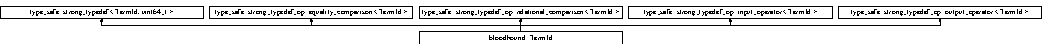
\includegraphics[height=0.592593cm]{structbloodhound_1_1TermId}
\end{center}
\end{figure}


The documentation for this struct was generated from the following file\+:\begin{DoxyCompactItemize}
\item 
include/\mbox{\hyperlink{index_8hpp}{index.\+hpp}}\end{DoxyCompactItemize}

\hypertarget{structbloodhound_1_1TermWeight}{}\section{bloodhound\+:\+:Term\+Weight Struct Reference}
\label{structbloodhound_1_1TermWeight}\index{bloodhound\+::\+Term\+Weight@{bloodhound\+::\+Term\+Weight}}


{\ttfamily \#include $<$index.\+hpp$>$}

\subsection*{Public Attributes}
\begin{DoxyCompactItemize}
\item 
\mbox{\hyperlink{structbloodhound_1_1TermId}{Term\+Id}} \mbox{\hyperlink{structbloodhound_1_1TermWeight_a8606421116b89015b89272bd5e2602a9}{term}}
\item 
\mbox{\hyperlink{structbloodhound_1_1Score}{Score}} \mbox{\hyperlink{structbloodhound_1_1TermWeight_a1abc2c53928fbaa8dcf617e72e1afced}{weight}}
\end{DoxyCompactItemize}


\subsection{Member Data Documentation}
\mbox{\Hypertarget{structbloodhound_1_1TermWeight_a8606421116b89015b89272bd5e2602a9}\label{structbloodhound_1_1TermWeight_a8606421116b89015b89272bd5e2602a9}} 
\index{bloodhound\+::\+Term\+Weight@{bloodhound\+::\+Term\+Weight}!term@{term}}
\index{term@{term}!bloodhound\+::\+Term\+Weight@{bloodhound\+::\+Term\+Weight}}
\subsubsection{\texorpdfstring{term}{term}}
{\footnotesize\ttfamily \mbox{\hyperlink{structbloodhound_1_1TermId}{Term\+Id}} bloodhound\+::\+Term\+Weight\+::term}

\mbox{\Hypertarget{structbloodhound_1_1TermWeight_a1abc2c53928fbaa8dcf617e72e1afced}\label{structbloodhound_1_1TermWeight_a1abc2c53928fbaa8dcf617e72e1afced}} 
\index{bloodhound\+::\+Term\+Weight@{bloodhound\+::\+Term\+Weight}!weight@{weight}}
\index{weight@{weight}!bloodhound\+::\+Term\+Weight@{bloodhound\+::\+Term\+Weight}}
\subsubsection{\texorpdfstring{weight}{weight}}
{\footnotesize\ttfamily \mbox{\hyperlink{structbloodhound_1_1Score}{Score}} bloodhound\+::\+Term\+Weight\+::weight}



The documentation for this struct was generated from the following file\+:\begin{DoxyCompactItemize}
\item 
include/\mbox{\hyperlink{index_8hpp}{index.\+hpp}}\end{DoxyCompactItemize}

\hypertarget{classbloodhound_1_1query_1_1ThresholdRetriever}{}\section{bloodhound\+:\+:query\+:\+:Threshold\+Retriever$<$ Posting\+List $>$ Class Template Reference}
\label{classbloodhound_1_1query_1_1ThresholdRetriever}\index{bloodhound\+::query\+::\+Threshold\+Retriever$<$ Posting\+List $>$@{bloodhound\+::query\+::\+Threshold\+Retriever$<$ Posting\+List $>$}}


{\ttfamily \#include $<$saat.\+hpp$>$}

Inheritance diagram for bloodhound\+:\+:query\+:\+:Threshold\+Retriever$<$ Posting\+List $>$\+:\begin{figure}[H]
\begin{center}
\leavevmode
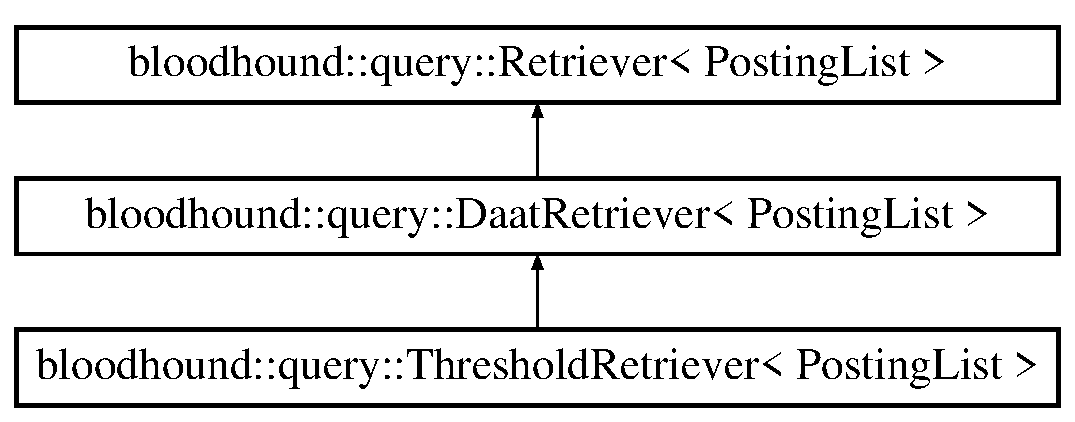
\includegraphics[height=3.000000cm]{classbloodhound_1_1query_1_1ThresholdRetriever}
\end{center}
\end{figure}
\subsection*{Public Member Functions}
\begin{DoxyCompactItemize}
\item 
\hyperlink{classbloodhound_1_1query_1_1ThresholdRetriever_a425d17d048e1fd3fd8157450c99df5bc}{Threshold\+Retriever} (std\+::size\+\_\+t collection\+\_\+size)
\item 
\hyperlink{structbloodhound_1_1Score}{Score} \hyperlink{classbloodhound_1_1query_1_1ThresholdRetriever_ac0a8731d270c477e04f24b89850a7d4a}{score\+\_\+with\+\_\+lookups} (\hyperlink{structbloodhound_1_1Doc}{Doc} doc, std\+::vector$<$ \hyperlink{structbloodhound_1_1Score}{Score} $>$ \&acc)
\item 
virtual std\+::vector$<$ \hyperlink{structbloodhound_1_1query_1_1Result}{Result} $>$ \hyperlink{classbloodhound_1_1query_1_1ThresholdRetriever_a06750450e1246e755ebad2d5dac6e8a8}{retrieve} (const std\+::vector$<$ \hyperlink{classbloodhound_1_1PostingList}{Posting\+List} $>$ \&term\+\_\+postings, const std\+::vector$<$ \hyperlink{structbloodhound_1_1Score}{Score} $>$ \&term\+\_\+weights, std\+::size\+\_\+t k)
\begin{DoxyCompactList}\small\item\em Retrieves top-\/k results for the given posting lists and term weights. \end{DoxyCompactList}\item 
virtual nlohmann\+::json \hyperlink{classbloodhound_1_1query_1_1ThresholdRetriever_aa21e5b44d70bfdf058e5f9c5a1abc008}{stats} ()
\end{DoxyCompactItemize}


\subsection{Detailed Description}
\subsubsection*{template$<$typename Posting\+List$>$\newline
class bloodhound\+::query\+::\+Threshold\+Retriever$<$ Posting\+List $>$}

Implementation of Fagin\textquotesingle{}s Threshold Algorithm.

Assumes that postings are sorted by their partial scores. 

\subsection{Constructor \& Destructor Documentation}
\mbox{\Hypertarget{classbloodhound_1_1query_1_1ThresholdRetriever_a425d17d048e1fd3fd8157450c99df5bc}\label{classbloodhound_1_1query_1_1ThresholdRetriever_a425d17d048e1fd3fd8157450c99df5bc}} 
\index{bloodhound\+::query\+::\+Threshold\+Retriever@{bloodhound\+::query\+::\+Threshold\+Retriever}!Threshold\+Retriever@{Threshold\+Retriever}}
\index{Threshold\+Retriever@{Threshold\+Retriever}!bloodhound\+::query\+::\+Threshold\+Retriever@{bloodhound\+::query\+::\+Threshold\+Retriever}}
\subsubsection{\texorpdfstring{Threshold\+Retriever()}{ThresholdRetriever()}}
{\footnotesize\ttfamily template$<$typename Posting\+List $>$ \\
\hyperlink{classbloodhound_1_1query_1_1ThresholdRetriever}{bloodhound\+::query\+::\+Threshold\+Retriever}$<$ \hyperlink{classbloodhound_1_1PostingList}{Posting\+List} $>$\+::\hyperlink{classbloodhound_1_1query_1_1ThresholdRetriever}{Threshold\+Retriever} (\begin{DoxyParamCaption}\item[{std\+::size\+\_\+t}]{collection\+\_\+size }\end{DoxyParamCaption})\hspace{0.3cm}{\ttfamily [inline]}}



\subsection{Member Function Documentation}
\mbox{\Hypertarget{classbloodhound_1_1query_1_1ThresholdRetriever_a06750450e1246e755ebad2d5dac6e8a8}\label{classbloodhound_1_1query_1_1ThresholdRetriever_a06750450e1246e755ebad2d5dac6e8a8}} 
\index{bloodhound\+::query\+::\+Threshold\+Retriever@{bloodhound\+::query\+::\+Threshold\+Retriever}!retrieve@{retrieve}}
\index{retrieve@{retrieve}!bloodhound\+::query\+::\+Threshold\+Retriever@{bloodhound\+::query\+::\+Threshold\+Retriever}}
\subsubsection{\texorpdfstring{retrieve()}{retrieve()}}
{\footnotesize\ttfamily template$<$typename Posting\+List $>$ \\
virtual std\+::vector$<$\hyperlink{structbloodhound_1_1query_1_1Result}{Result}$>$ \hyperlink{classbloodhound_1_1query_1_1ThresholdRetriever}{bloodhound\+::query\+::\+Threshold\+Retriever}$<$ \hyperlink{classbloodhound_1_1PostingList}{Posting\+List} $>$\+::retrieve (\begin{DoxyParamCaption}\item[{const std\+::vector$<$ \hyperlink{classbloodhound_1_1PostingList}{Posting\+List} $>$ \&}]{term\+\_\+postings,  }\item[{const std\+::vector$<$ \hyperlink{structbloodhound_1_1Score}{Score} $>$ \&}]{term\+\_\+weights,  }\item[{std\+::size\+\_\+t}]{k }\end{DoxyParamCaption})\hspace{0.3cm}{\ttfamily [inline]}, {\ttfamily [virtual]}}



Retrieves top-\/k results for the given posting lists and term weights. 



Reimplemented from \hyperlink{classbloodhound_1_1query_1_1DaatRetriever_ab80b4867fc263827dc2fdbe0965a2e8c}{bloodhound\+::query\+::\+Daat\+Retriever$<$ Posting\+List $>$}.

\mbox{\Hypertarget{classbloodhound_1_1query_1_1ThresholdRetriever_ac0a8731d270c477e04f24b89850a7d4a}\label{classbloodhound_1_1query_1_1ThresholdRetriever_ac0a8731d270c477e04f24b89850a7d4a}} 
\index{bloodhound\+::query\+::\+Threshold\+Retriever@{bloodhound\+::query\+::\+Threshold\+Retriever}!score\+\_\+with\+\_\+lookups@{score\+\_\+with\+\_\+lookups}}
\index{score\+\_\+with\+\_\+lookups@{score\+\_\+with\+\_\+lookups}!bloodhound\+::query\+::\+Threshold\+Retriever@{bloodhound\+::query\+::\+Threshold\+Retriever}}
\subsubsection{\texorpdfstring{score\+\_\+with\+\_\+lookups()}{score\_with\_lookups()}}
{\footnotesize\ttfamily template$<$typename Posting\+List $>$ \\
\hyperlink{structbloodhound_1_1Score}{Score} \hyperlink{classbloodhound_1_1query_1_1ThresholdRetriever}{bloodhound\+::query\+::\+Threshold\+Retriever}$<$ \hyperlink{classbloodhound_1_1PostingList}{Posting\+List} $>$\+::score\+\_\+with\+\_\+lookups (\begin{DoxyParamCaption}\item[{\hyperlink{structbloodhound_1_1Doc}{Doc}}]{doc,  }\item[{std\+::vector$<$ \hyperlink{structbloodhound_1_1Score}{Score} $>$ \&}]{acc }\end{DoxyParamCaption})\hspace{0.3cm}{\ttfamily [inline]}}

\mbox{\Hypertarget{classbloodhound_1_1query_1_1ThresholdRetriever_aa21e5b44d70bfdf058e5f9c5a1abc008}\label{classbloodhound_1_1query_1_1ThresholdRetriever_aa21e5b44d70bfdf058e5f9c5a1abc008}} 
\index{bloodhound\+::query\+::\+Threshold\+Retriever@{bloodhound\+::query\+::\+Threshold\+Retriever}!stats@{stats}}
\index{stats@{stats}!bloodhound\+::query\+::\+Threshold\+Retriever@{bloodhound\+::query\+::\+Threshold\+Retriever}}
\subsubsection{\texorpdfstring{stats()}{stats()}}
{\footnotesize\ttfamily template$<$typename Posting\+List $>$ \\
virtual nlohmann\+::json \hyperlink{classbloodhound_1_1query_1_1ThresholdRetriever}{bloodhound\+::query\+::\+Threshold\+Retriever}$<$ \hyperlink{classbloodhound_1_1PostingList}{Posting\+List} $>$\+::stats (\begin{DoxyParamCaption}{ }\end{DoxyParamCaption})\hspace{0.3cm}{\ttfamily [inline]}, {\ttfamily [virtual]}}



Reimplemented from \hyperlink{classbloodhound_1_1query_1_1Retriever_a58da32a5139b980ba874f8b5e6bb89ec}{bloodhound\+::query\+::\+Retriever$<$ Posting\+List $>$}.



The documentation for this class was generated from the following file\+:\begin{DoxyCompactItemize}
\item 
include/\hyperlink{saat_8hpp}{saat.\+hpp}\end{DoxyCompactItemize}

\hypertarget{classbloodhound_1_1query_1_1WandRetriever}{}\section{bloodhound\+:\+:query\+:\+:Wand\+Retriever$<$ Posting\+List $>$ Class Template Reference}
\label{classbloodhound_1_1query_1_1WandRetriever}\index{bloodhound\+::query\+::\+Wand\+Retriever$<$ Posting\+List $>$@{bloodhound\+::query\+::\+Wand\+Retriever$<$ Posting\+List $>$}}


W\+A\+ND (Weak-\/\+A\+ND) query retriever.  




{\ttfamily \#include $<$retrievers.\+hpp$>$}

Inheritance diagram for bloodhound\+:\+:query\+:\+:Wand\+Retriever$<$ Posting\+List $>$\+:\begin{figure}[H]
\begin{center}
\leavevmode
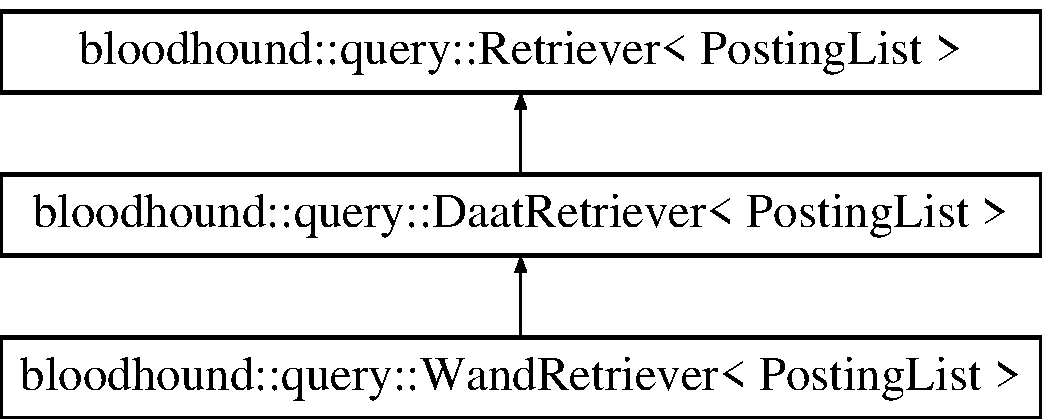
\includegraphics[height=3.000000cm]{classbloodhound_1_1query_1_1WandRetriever}
\end{center}
\end{figure}
\subsection*{Public Member Functions}
\begin{DoxyCompactItemize}
\item 
virtual std\+::vector$<$ \mbox{\hyperlink{structbloodhound_1_1query_1_1Result}{Result}} $>$ \mbox{\hyperlink{classbloodhound_1_1query_1_1WandRetriever_a5f3068bc363c16c5b7255a925ea5af8c}{retrieve}} (const std\+::vector$<$ \mbox{\hyperlink{classbloodhound_1_1PostingList}{Posting\+List}} $>$ \&term\+\_\+postings, const std\+::vector$<$ \mbox{\hyperlink{structbloodhound_1_1Score}{Score}} $>$ \&term\+\_\+weights, std\+::size\+\_\+t k)
\begin{DoxyCompactList}\small\item\em Retrieves top-\/k results for the given posting lists and term weights. \end{DoxyCompactList}\item 
virtual nlohmann\+::json \mbox{\hyperlink{classbloodhound_1_1query_1_1WandRetriever_a1e593c2cddb2ca4f2415c59ca26e6a36}{stats}} ()
\end{DoxyCompactItemize}


\subsection{Detailed Description}
\subsubsection*{template$<$typename Posting\+List$>$\newline
class bloodhound\+::query\+::\+Wand\+Retriever$<$ Posting\+List $>$}

W\+A\+ND (Weak-\/\+A\+ND) query retriever. 

\subsection{Member Function Documentation}
\mbox{\Hypertarget{classbloodhound_1_1query_1_1WandRetriever_a5f3068bc363c16c5b7255a925ea5af8c}\label{classbloodhound_1_1query_1_1WandRetriever_a5f3068bc363c16c5b7255a925ea5af8c}} 
\index{bloodhound\+::query\+::\+Wand\+Retriever@{bloodhound\+::query\+::\+Wand\+Retriever}!retrieve@{retrieve}}
\index{retrieve@{retrieve}!bloodhound\+::query\+::\+Wand\+Retriever@{bloodhound\+::query\+::\+Wand\+Retriever}}
\subsubsection{\texorpdfstring{retrieve()}{retrieve()}}
{\footnotesize\ttfamily template$<$typename Posting\+List $>$ \\
virtual std\+::vector$<$\mbox{\hyperlink{structbloodhound_1_1query_1_1Result}{Result}}$>$ \mbox{\hyperlink{classbloodhound_1_1query_1_1WandRetriever}{bloodhound\+::query\+::\+Wand\+Retriever}}$<$ \mbox{\hyperlink{classbloodhound_1_1PostingList}{Posting\+List}} $>$\+::retrieve (\begin{DoxyParamCaption}\item[{const std\+::vector$<$ \mbox{\hyperlink{classbloodhound_1_1PostingList}{Posting\+List}} $>$ \&}]{term\+\_\+postings,  }\item[{const std\+::vector$<$ \mbox{\hyperlink{structbloodhound_1_1Score}{Score}} $>$ \&}]{term\+\_\+weights,  }\item[{std\+::size\+\_\+t}]{k }\end{DoxyParamCaption})\hspace{0.3cm}{\ttfamily [inline]}, {\ttfamily [virtual]}}



Retrieves top-\/k results for the given posting lists and term weights. 



Reimplemented from \mbox{\hyperlink{classbloodhound_1_1query_1_1DaatRetriever_ab80b4867fc263827dc2fdbe0965a2e8c}{bloodhound\+::query\+::\+Daat\+Retriever$<$ Posting\+List $>$}}.

\mbox{\Hypertarget{classbloodhound_1_1query_1_1WandRetriever_a1e593c2cddb2ca4f2415c59ca26e6a36}\label{classbloodhound_1_1query_1_1WandRetriever_a1e593c2cddb2ca4f2415c59ca26e6a36}} 
\index{bloodhound\+::query\+::\+Wand\+Retriever@{bloodhound\+::query\+::\+Wand\+Retriever}!stats@{stats}}
\index{stats@{stats}!bloodhound\+::query\+::\+Wand\+Retriever@{bloodhound\+::query\+::\+Wand\+Retriever}}
\subsubsection{\texorpdfstring{stats()}{stats()}}
{\footnotesize\ttfamily template$<$typename Posting\+List $>$ \\
virtual nlohmann\+::json \mbox{\hyperlink{classbloodhound_1_1query_1_1WandRetriever}{bloodhound\+::query\+::\+Wand\+Retriever}}$<$ \mbox{\hyperlink{classbloodhound_1_1PostingList}{Posting\+List}} $>$\+::stats (\begin{DoxyParamCaption}{ }\end{DoxyParamCaption})\hspace{0.3cm}{\ttfamily [inline]}, {\ttfamily [virtual]}}



Reimplemented from \mbox{\hyperlink{classbloodhound_1_1query_1_1Retriever_a58da32a5139b980ba874f8b5e6bb89ec}{bloodhound\+::query\+::\+Retriever$<$ Posting\+List $>$}}.



The documentation for this class was generated from the following file\+:\begin{DoxyCompactItemize}
\item 
include/\mbox{\hyperlink{retrievers_8hpp}{retrievers.\+hpp}}\end{DoxyCompactItemize}

\chapter{File Documentation}
\hypertarget{index_8hpp}{}\section{include/index.hpp File Reference}
\label{index_8hpp}\index{include/index.\+hpp@{include/index.\+hpp}}
{\ttfamily \#include $<$experimental/filesystem$>$}\newline
{\ttfamily \#include $<$fstream$>$}\newline
{\ttfamily \#include $<$gsl/gsl\+\_\+assert$>$}\newline
{\ttfamily \#include $<$gsl/span$>$}\newline
{\ttfamily \#include $<$iostream$>$}\newline
{\ttfamily \#include $<$nlohmann/json.\+hpp$>$}\newline
{\ttfamily \#include $<$type\+\_\+safe/strong\+\_\+typedef.\+hpp$>$}\newline
{\ttfamily \#include $<$unordered\+\_\+map$>$}\newline
\subsection*{Classes}
\begin{DoxyCompactItemize}
\item 
struct \mbox{\hyperlink{structbloodhound_1_1TermId}{bloodhound\+::\+Term\+Id}}
\item 
struct \mbox{\hyperlink{structbloodhound_1_1Offset}{bloodhound\+::\+Offset}}
\item 
struct \mbox{\hyperlink{structbloodhound_1_1RelativeOffset}{bloodhound\+::\+Relative\+Offset}}
\item 
struct \mbox{\hyperlink{structbloodhound_1_1Score}{bloodhound\+::\+Score}}
\item 
struct \mbox{\hyperlink{structbloodhound_1_1Doc}{bloodhound\+::\+Doc}}
\item 
struct \mbox{\hyperlink{structbloodhound_1_1Posting}{bloodhound\+::\+Posting}}
\item 
struct \mbox{\hyperlink{structbloodhound_1_1doc__equal__to}{bloodhound\+::doc\+\_\+equal\+\_\+to$<$ Posting $>$}}
\item 
struct \mbox{\hyperlink{structbloodhound_1_1add__postings}{bloodhound\+::add\+\_\+postings$<$ Posting $>$}}
\item 
struct \mbox{\hyperlink{structbloodhound_1_1score__greater}{bloodhound\+::score\+\_\+greater$<$ Posting $>$}}
\item 
struct \mbox{\hyperlink{structbloodhound_1_1TermWeight}{bloodhound\+::\+Term\+Weight}}
\item 
class \mbox{\hyperlink{classbloodhound_1_1PostingList}{bloodhound\+::\+Posting\+List}}
\item 
struct \mbox{\hyperlink{structbloodhound_1_1PostingList_1_1const__iterator}{bloodhound\+::\+Posting\+List\+::const\+\_\+iterator}}
\item 
struct \mbox{\hyperlink{structbloodhound_1_1PostingList_1_1iterator}{bloodhound\+::\+Posting\+List\+::iterator}}
\item 
struct \mbox{\hyperlink{structstd_1_1hash_3_01bloodhound_1_1TermId_01_4}{std\+::hash$<$ bloodhound\+::\+Term\+Id $>$}}
\item 
struct \mbox{\hyperlink{structstd_1_1hash_3_01bloodhound_1_1Score_01_4}{std\+::hash$<$ bloodhound\+::\+Score $>$}}
\item 
struct \mbox{\hyperlink{structstd_1_1hash_3_01bloodhound_1_1Doc_01_4}{std\+::hash$<$ bloodhound\+::\+Doc $>$}}
\item 
struct \mbox{\hyperlink{structbloodhound_1_1index_1_1PostingListHeader}{bloodhound\+::index\+::\+Posting\+List\+Header}}
\item 
class \mbox{\hyperlink{classbloodhound_1_1index_1_1InMemoryPostingPolicy}{bloodhound\+::index\+::\+In\+Memory\+Posting\+Policy}}
\item 
class \mbox{\hyperlink{classbloodhound_1_1index_1_1Index}{bloodhound\+::index\+::\+Index$<$ Posting\+Policy $>$}}
\end{DoxyCompactItemize}
\subsection*{Namespaces}
\begin{DoxyCompactItemize}
\item 
 \mbox{\hyperlink{namespacebloodhound}{bloodhound}}
\item 
 \mbox{\hyperlink{namespacestd}{std}}
\item 
 \mbox{\hyperlink{namespacebloodhound_1_1index}{bloodhound\+::index}}
\end{DoxyCompactItemize}
\subsection*{Typedefs}
\begin{DoxyCompactItemize}
\item 
using \mbox{\hyperlink{namespacebloodhound_ae863daa54e3092bd2bc335e70f7a9dd7}{bloodhound\+::\+Accumulator\+Array}} = std\+::vector$<$ Score $>$
\item 
using \mbox{\hyperlink{namespacebloodhound_a94032a3533df0a1b6d3435bad57e6499}{bloodhound\+::\+Lexicon}} = std\+::unordered\+\_\+map$<$ Term\+Id, Offset $>$
\item 
using \mbox{\hyperlink{namespacebloodhound_a687d80c6f992eba8b820bf30a482f4b4}{bloodhound\+::\+Max\+Scores}} = std\+::unordered\+\_\+map$<$ Term\+Id, Score $>$
\end{DoxyCompactItemize}
\subsection*{Functions}
\begin{DoxyCompactItemize}
\item 
bool \mbox{\hyperlink{namespacebloodhound_aa37ad87847e4da8983f626e6c5779c73}{bloodhound\+::operator==}} (const Posting \&a, const Posting \&b)
\item 
bool \mbox{\hyperlink{namespacebloodhound_a4a683ebe3ff767a829b87a89bade978c}{bloodhound\+::operator$>$}} (const Posting \&a, const Posting \&b)
\item 
bool \mbox{\hyperlink{namespacebloodhound_ae20cf3f97304dde56dd526eaa08c41dc}{bloodhound\+::operator$<$}} (const Posting \&a, const Posting \&b)
\item 
Posting \mbox{\hyperlink{namespacebloodhound_a0ee8a7512bc2dea6326445fa8b7509b2}{bloodhound\+::operator$\ast$}} (const Posting \&p, Score weight)
\item 
std\+::ostream \& \mbox{\hyperlink{namespacebloodhound_a1422cc04658f6eb8616381224186059f}{bloodhound\+::operator$<$$<$}} (std\+::ostream \&os, const Posting \&p)
\item 
Posting \mbox{\hyperlink{namespacebloodhound_a0b07d73bf298a56b219b270d5fa70b83}{bloodhound\+::operator+}} (const Posting \&lhs, const Posting \&rhs)
\item 
std\+::vector$<$ char $>$ \mbox{\hyperlink{namespacebloodhound_1_1index_a4b6f89a17c10bf2927aff24df7081bb3}{bloodhound\+::index\+::read\+\_\+file}} (fs\+::path filepath)
\item 
Index$<$ In\+Memory\+Posting\+Policy $>$ \mbox{\hyperlink{namespacebloodhound_1_1index_ac508959a4f3ab5ce65d62f1c294359e2}{bloodhound\+::index\+::build\+\_\+index\+\_\+from\+\_\+ids}} (const std\+::vector$<$ std\+::vector$<$ Term\+Weight $>$$>$ \&input)
\item 
Index$<$ In\+Memory\+Posting\+Policy $>$ \mbox{\hyperlink{namespacebloodhound_1_1index_a306f62c55e8d06a9703f552f7cf312c5}{bloodhound\+::index\+::sorted\+\_\+index}} (const Index$<$ In\+Memory\+Posting\+Policy $>$ \&index)
\end{DoxyCompactItemize}

\hypertarget{query_8hpp}{}\section{include/query.hpp File Reference}
\label{query_8hpp}\index{include/query.\+hpp@{include/query.\+hpp}}
{\ttfamily \#include $<$algorithm$>$}\newline
{\ttfamily \#include $<$chrono$>$}\newline
{\ttfamily \#include $<$iostream$>$}\newline
{\ttfamily \#include $<$math.\+h$>$}\newline
{\ttfamily \#include $<$type\+\_\+traits$>$}\newline
{\ttfamily \#include \char`\"{}debug\+\_\+assert.\+hpp\char`\"{}}\newline
{\ttfamily \#include \char`\"{}index.\+hpp\char`\"{}}\newline
{\ttfamily \#include \char`\"{}irkit/heap.\+hpp\char`\"{}}\newline
\subsection*{Classes}
\begin{DoxyCompactItemize}
\item 
struct \hyperlink{structbloodhound_1_1query_1_1has__posting__iterator}{bloodhound\+::query\+::has\+\_\+posting\+\_\+iterator$<$ T, typename $>$}
\item 
struct \hyperlink{structbloodhound_1_1query_1_1has__posting__iterator_3_01T_00_01std_1_1enable__if__t_3_01std_1_1i3aad327a30d60305d06d5c73680c1a38}{bloodhound\+::query\+::has\+\_\+posting\+\_\+iterator$<$ T, std\+::enable\+\_\+if\+\_\+t$<$ std\+::is\+\_\+convertible$<$ decltype(std\+::declval$<$ T \& $>$().\+end()), typename T\+::iterator $>$\+::value \&\&std\+::is\+\_\+convertible$<$ decltype(std\+::declval$<$ T \& $>$().\+begin()), typename T\+::iterator $>$\+::value \&\&std\+::is\+\_\+convertible$<$ decltype($\ast$std\+::declval$<$ T \& $>$().\+begin()), Posting \& $>$\+::value \&\&std\+::is\+\_\+convertible$<$ decltype($\ast$std\+::declval$<$ T \& $>$().\+end()), Posting \& $>$\+::value $>$ $>$}
\item 
struct \hyperlink{structbloodhound_1_1query_1_1has__iterator}{bloodhound\+::query\+::has\+\_\+iterator$<$ T, typename $>$}
\item 
struct \hyperlink{structbloodhound_1_1query_1_1has__iterator_3_01T_00_01void__t_3_01typename_01T_1_1iterator_01_4_01_4}{bloodhound\+::query\+::has\+\_\+iterator$<$ T, void\+\_\+t$<$ typename T\+::iterator $>$ $>$}
\item 
struct \hyperlink{structbloodhound_1_1query_1_1debug}{bloodhound\+::query\+::debug}
\item 
struct \hyperlink{structbloodhound_1_1query_1_1Result}{bloodhound\+::query\+::\+Result}
\item 
class \hyperlink{classbloodhound_1_1query_1_1Retriever}{bloodhound\+::query\+::\+Retriever$<$ Posting\+List $>$}
\begin{DoxyCompactList}\small\item\em A base abstract super-\/class of all document retrievers. \end{DoxyCompactList}\end{DoxyCompactItemize}
\subsection*{Namespaces}
\begin{DoxyCompactItemize}
\item 
 \hyperlink{namespacebloodhound_1_1query}{bloodhound\+::query}
\end{DoxyCompactItemize}
\subsection*{Typedefs}
\begin{DoxyCompactItemize}
\item 
{\footnotesize template$<$typename T $>$ }\\using \hyperlink{namespacebloodhound_1_1query_afd658a38b784a8187f8782905cb901e6}{bloodhound\+::query\+::void\+\_\+t} = void
\end{DoxyCompactItemize}
\subsection*{Functions}
\begin{DoxyCompactItemize}
\item 
{\footnotesize template$<$typename Compare  = std\+::less$<$\+Score$>$, typename Mapping  = irkit\+::\+Empty\+Mapping$>$ }\\std\+::vector$<$ Result $>$ \hyperlink{namespacebloodhound_1_1query_a1ec90cdc5f56c17431fd2e2cd2acbb93}{bloodhound\+::query\+::heap\+\_\+to\+\_\+results} (\hyperlink{classirkit_1_1Heap}{irkit\+::\+Heap}$<$ Score, Doc, Compare, Mapping $>$ \&heap)
\begin{DoxyCompactList}\small\item\em Converts a min-\/heap of top-\/scored documents to a sorted vector of results. \end{DoxyCompactList}\end{DoxyCompactItemize}

\hypertarget{retrievers_8hpp}{}\section{include/retrievers.hpp File Reference}
\label{retrievers_8hpp}\index{include/retrievers.\+hpp@{include/retrievers.\+hpp}}
{\ttfamily \#include $<$list$>$}\newline
{\ttfamily \#include $<$range/v3/numeric/accumulate.\+hpp$>$}\newline
{\ttfamily \#include $<$range/v3/view/transform.\+hpp$>$}\newline
{\ttfamily \#include $<$range/v3/view/zip.\+hpp$>$}\newline
{\ttfamily \#include $<$set$>$}\newline
{\ttfamily \#include \char`\"{}irkit/daat.\+hpp\char`\"{}}\newline
{\ttfamily \#include \char`\"{}irkit/taat.\+hpp\char`\"{}}\newline
{\ttfamily \#include \char`\"{}query.\+hpp\char`\"{}}\newline
\subsection*{Classes}
\begin{DoxyCompactItemize}
\item 
class \hyperlink{classbloodhound_1_1query_1_1DaatRetriever}{bloodhound\+::query\+::\+Daat\+Retriever$<$ Posting\+List $>$}
\begin{DoxyCompactList}\small\item\em Document-\/at-\/a-\/time query processor. \end{DoxyCompactList}\item 
struct \hyperlink{structbloodhound_1_1query_1_1DaatRetriever_1_1IteratorPair}{bloodhound\+::query\+::\+Daat\+Retriever$<$ Posting\+List $>$\+::\+Iterator\+Pair}
\begin{DoxyCompactList}\small\item\em Current and end iterators of the same posting list. \end{DoxyCompactList}\item 
class \hyperlink{classbloodhound_1_1query_1_1WandRetriever}{bloodhound\+::query\+::\+Wand\+Retriever$<$ Posting\+List $>$}
\begin{DoxyCompactList}\small\item\em W\+A\+ND (Weak-\/\+A\+ND) query retriever. \end{DoxyCompactList}\item 
class \hyperlink{classbloodhound_1_1query_1_1MaxScoreRetriever}{bloodhound\+::query\+::\+Max\+Score\+Retriever$<$ Posting\+List $>$}
\item 
class \hyperlink{classbloodhound_1_1query_1_1TaatRetriever}{bloodhound\+::query\+::\+Taat\+Retriever$<$ Posting\+List, prefetch, init\+\_\+gap, acc\+\_\+block\+\_\+size $>$}
\item 
class \hyperlink{classbloodhound_1_1query_1_1MaxScoreNonEssentials}{bloodhound\+::query\+::\+Max\+Score\+Non\+Essentials$<$ Posting\+List $>$}
\item 
class \hyperlink{classbloodhound_1_1query_1_1RawTaatRetriever}{bloodhound\+::query\+::\+Raw\+Taat\+Retriever$<$ Posting\+List $>$}
\item 
class \hyperlink{classbloodhound_1_1query_1_1TaatMaxScoreRetriever}{bloodhound\+::query\+::\+Taat\+Max\+Score\+Retriever$<$ Posting\+List $>$}
\end{DoxyCompactItemize}
\subsection*{Namespaces}
\begin{DoxyCompactItemize}
\item 
 \hyperlink{namespacebloodhound_1_1query}{bloodhound\+::query}
\end{DoxyCompactItemize}
\subsection*{Typedefs}
\begin{DoxyCompactItemize}
\item 
using \hyperlink{namespacebloodhound_1_1query_aa67214af106292b2483995adea986b08}{bloodhound\+::query\+::\+Query\+Id} = unsigned char
\end{DoxyCompactItemize}

\hypertarget{run_8hpp}{}\section{include/run.hpp File Reference}
\label{run_8hpp}\index{include/run.\+hpp@{include/run.\+hpp}}
{\ttfamily \#include $<$string$>$}\newline
{\ttfamily \#include \char`\"{}index.\+hpp\char`\"{}}\newline
{\ttfamily \#include \char`\"{}irkit/utils.\+hpp\char`\"{}}\newline
{\ttfamily \#include \char`\"{}query.\+hpp\char`\"{}}\newline
{\ttfamily \#include \char`\"{}retrievers.\+hpp\char`\"{}}\newline
{\ttfamily \#include \char`\"{}run.\+hpp\char`\"{}}\newline
\subsection*{Functions}
\begin{DoxyCompactItemize}
\item 
std\+::vector$<$ std\+::tuple$<$ \mbox{\hyperlink{structbloodhound_1_1TermId}{Term\+Id}}, \mbox{\hyperlink{structbloodhound_1_1Score}{Score}} $>$ $>$ \mbox{\hyperlink{run_8hpp_a87489cd09b789da5adbd8285a5098520}{parse\+\_\+query}} (std\+::string \&query\+\_\+line)
\item 
std\+::vector$<$ std\+::string $>$ \mbox{\hyperlink{run_8hpp_a3ef37056433b3eb491952d765d6ca4ce}{load\+\_\+titles}} (fs\+::path titles\+\_\+path)
\item 
std\+::vector$<$ \mbox{\hyperlink{structbloodhound_1_1query_1_1Result}{query\+::\+Result}} $>$ \mbox{\hyperlink{run_8hpp_a2f2551f30f22dc8d3249d1162a94c75a}{to\+\_\+results}} (std\+::vector$<$ \mbox{\hyperlink{structbloodhound_1_1Posting}{Posting}} $>$ \&postings)
\item 
void \mbox{\hyperlink{run_8hpp_a8a96b78740ebdc82301565813ae03600}{run\+\_\+with}} (std\+::vector$<$ \mbox{\hyperlink{structbloodhound_1_1query_1_1Result}{query\+::\+Result}} $>$($\ast$run)(const std\+::vector$<$ \mbox{\hyperlink{classbloodhound_1_1PostingList}{Posting\+List}} $>$ \&, const std\+::vector$<$ \mbox{\hyperlink{structbloodhound_1_1Score}{Score}} $>$ \&, std\+::size\+\_\+t, \mbox{\hyperlink{classbloodhound_1_1index_1_1Index}{index\+::\+Index}}$<$$>$ \&), \mbox{\hyperlink{classbloodhound_1_1index_1_1Index}{index\+::\+Index}}$<$$>$ \&ind, fs\+::path query\+\_\+file)
\end{DoxyCompactItemize}


\subsection{Function Documentation}
\mbox{\Hypertarget{run_8hpp_a3ef37056433b3eb491952d765d6ca4ce}\label{run_8hpp_a3ef37056433b3eb491952d765d6ca4ce}} 
\index{run.\+hpp@{run.\+hpp}!load\+\_\+titles@{load\+\_\+titles}}
\index{load\+\_\+titles@{load\+\_\+titles}!run.\+hpp@{run.\+hpp}}
\subsubsection{\texorpdfstring{load\+\_\+titles()}{load\_titles()}}
{\footnotesize\ttfamily std\+::vector$<$std\+::string$>$ load\+\_\+titles (\begin{DoxyParamCaption}\item[{fs\+::path}]{titles\+\_\+path }\end{DoxyParamCaption})}

\mbox{\Hypertarget{run_8hpp_a87489cd09b789da5adbd8285a5098520}\label{run_8hpp_a87489cd09b789da5adbd8285a5098520}} 
\index{run.\+hpp@{run.\+hpp}!parse\+\_\+query@{parse\+\_\+query}}
\index{parse\+\_\+query@{parse\+\_\+query}!run.\+hpp@{run.\+hpp}}
\subsubsection{\texorpdfstring{parse\+\_\+query()}{parse\_query()}}
{\footnotesize\ttfamily std\+::vector$<$std\+::tuple$<$\mbox{\hyperlink{structbloodhound_1_1TermId}{Term\+Id}}, \mbox{\hyperlink{structbloodhound_1_1Score}{Score}}$>$ $>$ parse\+\_\+query (\begin{DoxyParamCaption}\item[{std\+::string \&}]{query\+\_\+line }\end{DoxyParamCaption})}

\mbox{\Hypertarget{run_8hpp_a8a96b78740ebdc82301565813ae03600}\label{run_8hpp_a8a96b78740ebdc82301565813ae03600}} 
\index{run.\+hpp@{run.\+hpp}!run\+\_\+with@{run\+\_\+with}}
\index{run\+\_\+with@{run\+\_\+with}!run.\+hpp@{run.\+hpp}}
\subsubsection{\texorpdfstring{run\+\_\+with()}{run\_with()}}
{\footnotesize\ttfamily void run\+\_\+with (\begin{DoxyParamCaption}\item[{std\+::vector$<$ \mbox{\hyperlink{structbloodhound_1_1query_1_1Result}{query\+::\+Result}} $>$($\ast$)(const std\+::vector$<$ \mbox{\hyperlink{classbloodhound_1_1PostingList}{Posting\+List}} $>$ \&, const std\+::vector$<$ \mbox{\hyperlink{structbloodhound_1_1Score}{Score}} $>$ \&, std\+::size\+\_\+t, \mbox{\hyperlink{classbloodhound_1_1index_1_1Index}{index\+::\+Index}}$<$$>$ \&)}]{run,  }\item[{\mbox{\hyperlink{classbloodhound_1_1index_1_1Index}{index\+::\+Index}}$<$$>$ \&}]{ind,  }\item[{fs\+::path}]{query\+\_\+file }\end{DoxyParamCaption})}

\mbox{\Hypertarget{run_8hpp_a2f2551f30f22dc8d3249d1162a94c75a}\label{run_8hpp_a2f2551f30f22dc8d3249d1162a94c75a}} 
\index{run.\+hpp@{run.\+hpp}!to\+\_\+results@{to\+\_\+results}}
\index{to\+\_\+results@{to\+\_\+results}!run.\+hpp@{run.\+hpp}}
\subsubsection{\texorpdfstring{to\+\_\+results()}{to\_results()}}
{\footnotesize\ttfamily std\+::vector$<$\mbox{\hyperlink{structbloodhound_1_1query_1_1Result}{query\+::\+Result}}$>$ to\+\_\+results (\begin{DoxyParamCaption}\item[{std\+::vector$<$ \mbox{\hyperlink{structbloodhound_1_1Posting}{Posting}} $>$ \&}]{postings }\end{DoxyParamCaption})}


\hypertarget{saat_8hpp}{}\section{include/saat.hpp File Reference}
\label{saat_8hpp}\index{include/saat.\+hpp@{include/saat.\+hpp}}
{\ttfamily \#include $<$assert.\+h$>$}\newline
{\ttfamily \#include $<$math.\+h$>$}\newline
{\ttfamily \#include \char`\"{}debug\+\_\+assert.\+hpp\char`\"{}}\newline
{\ttfamily \#include \char`\"{}irkit/daat.\+hpp\char`\"{}}\newline
{\ttfamily \#include \char`\"{}irkit/taat.\+hpp\char`\"{}}\newline
{\ttfamily \#include \char`\"{}query.\+hpp\char`\"{}}\newline
{\ttfamily \#include \char`\"{}retrievers.\+hpp\char`\"{}}\newline
\subsection*{Classes}
\begin{DoxyCompactItemize}
\item 
class \mbox{\hyperlink{classbloodhound_1_1query_1_1ExactSaatRetriever}{bloodhound\+::query\+::\+Exact\+Saat\+Retriever$<$ Posting\+List $>$}}
\item 
class \mbox{\hyperlink{classbloodhound_1_1query_1_1ThresholdRetriever}{bloodhound\+::query\+::\+Threshold\+Retriever$<$ Posting\+List $>$}}
\end{DoxyCompactItemize}
\subsection*{Namespaces}
\begin{DoxyCompactItemize}
\item 
 \mbox{\hyperlink{namespacebloodhound_1_1query}{bloodhound\+::query}}
\end{DoxyCompactItemize}

%--- End generated contents ---

% Index
\backmatter
\newpage
\phantomsection
\clearemptydoublepage
\addcontentsline{toc}{chapter}{Index}
\printindex

\end{document}
